% example for dissertation.sty

\documentclass[
  % Replace oneside by twoside if you are printing your thesis on both sides
  % of the paper, leave as is for single sided prints or for viewing on screen.
  oneside,
  11pt, a4paper,
  footinclude=true,
  headinclude=true,
  cleardoublepage=empty
]{scrbook}


\usepackage{dissertation}


% ACRONYMS -----------------------------------------------------

%import the necessary package with some options
\usepackage[acronym,nonumberlist,nomain]{glossaries}

%enable the following to avoid links from the acronym usage to the list
%\glsdisablehyper

%displays the first use of an acronym in italic
\defglsdisplayfirst[\acronymtype]{\emph{#1#4}}

%the style of the Glossary
%\setglossarystyle{listgroup}

%set the name for the acronym entries page
\renewcommand{\glossaryname}{Acronyms}

%this shall be the last thing in the acronym configuration!!
%
\makeglossaries

%load acronyms file
%\loadglsentries[\acronymtype]{sec/acronyms}

%% **MORE INFO** %%

%to add the acronyms list add the following where you want to print it:
%\printglossary[type=\acronymtype]
%\clearpage
%\thispagestyle{empty}

%to use an acronym:
%\gls{qps}

% compile the thesis in command line with the following command sequence:
% pdlatex dissertation.tex
% makeglossaries dissertation
% bibtex dissertation
% pdlatex dissertation.tex
% pdlatex dissertation.tex

% ----------------------------------------------------------------

% Title
\titleA{Development of a system}
\titleB{compliant with the Application-layer}
\titleC{Traffic Optimization protocol}
% Author
\author{Paulo Edgar Mendes Caldas}

\supervisor{Pedro Nuno Miranda de Sousa}
%\cosupervisor{}

% University (uncomment if you need to change default values)
% \def\school{Escola de Engenharia}
% \def\department{Departamento de Inform\'{a}tica}
% \def\university{Universidade do Minho}
\def\masterdegree{Informatics Engineering}

% Date
\date{\myear} % change to text if date is not today

% Keywords
%\keywords{master thesis}

% Glossaries & Acronyms
%\makeglossaries  %  either use this ...


%!TEX root = ../dissertation.tex

\newacronym{id}{ID}{Identifier}
\newacronym{rfc}{RFC}{Request for Comments}
\newacronym{p2p}{P2P}{Peer-to-Peer}
\newacronym{isp}{ISP}{Internet Service Provider}
\newacronym{as}{AS}{Autonomous System}
\newacronym{cdn}{CDN}{Content Distribution Network}
\newacronym{emea}{EMEA}{Europe, the Middle East and Africa}
\newacronym{qos}{QoS}{Quality of Service}
\newacronym{ietf}{IETF}{Internet Engineering Task Force}
\newacronym{dht}{DHT}{Distributed Hash Table}
\newacronym{can}{CAN}{Content Addressable Network}
\newacronym{qoe}{QoE}{Quality of Experience}
\newacronym{igp}{IGP}{Interior Gateway Protocol}
\newacronym{egp}{EGP}{Exterior Gateway Protocol}
\newacronym{tcp}{TCP}{Transmission Control Protocol}
\newacronym{mtr}{MTR}{Multi-Topology Routing}
\newacronym{mpls}{MPLS}{Multiprotocol Label Switching}
\newacronym{diffserv}{DiffServ}{Differentiated services}
\newacronym{cdni}{CDNI}{Content Distribution Network Interconnection}
\newacronym{sdn}{SDN}{Software Defined Networking}
\newacronym{rtt}{RTT}{Round-Trip Time}
\newacronym{ospf}{OSPF}{Open Shortest Path First}
\newacronym{snmp}{SNMP}{Simple Network Management Protocol}
\newacronym{rbac}{RBAC}{Role-Based Access Control }
\newacronym{acl}{ACL}{Access-Control List}
\newacronym{ipv4}{ipv4}{Internet Protocol version 4}
\newacronym{ipv6}{ipv6}{Internet Protocol version 6}
\newacronym{adsl}{ADSL}{Asymmetric digital subscriber line}
\newacronym{mac}{MAC}{Media Access Control}
\newacronym{ird}{IRD}{Information Resource Directory}
\newacronym{alto}{ALTO}{Application-Layer Traffic Optimization}
\newacronym{padis}{PaDIS}{Provider-Aided Distance Information System}
\newacronym{cate}{CaTE}{Content-Aware Traffic Engineering}
\newacronym{netpaas}{NetPaaS}{Network Platform as a Service}
\newacronym{xmpp}{XMPP}{Extensible Messaging and Presence Protocol}
\newacronym[\glslongpluralkey={Points of Presence}]{pop}{PoP}{Points of Presence}
\newacronym{cpu}{CPU}{Central Processing Unit}
\newacronym{ram}{RAM}{Random-Access Memory}
\newacronym{pid}{PID}{Provider-Defined Identifier}
\newacronym{ane}{ANE}{Abstract Network Element}
\newacronym{sql}{SQL}{Structured Query Language}
\newacronym{doh}{DoH}{DNS over HTTPS}
\newacronym{netconf}{NETCONF}{Network Configuration Protocol}
\newacronym{ted}{TED}{Traffic Engineering Database}
\newacronym{lspd}{LSPD}{Label Switched Path Database}
\newacronym{dns}{DNS}{Domain Name System}
\newacronym{mvc}{MVC}{Model-View-Controller}
\newacronym{rest}{REST}{Representational state transfer}
\newacronym{api}{API}{Application Programming Interface}
\newacronym{json}{JSON}{JavaScript Object Notation}
\newacronym{ip}{IP}{Internet Protocol}
\newacronym{http}{HTTP}{Hypertext Transfer Protocol}
\newacronym{https}{HTTPS}{Hypertext Transfer Protocol Secure}
\newacronym{tls}{TLS}{Transport Layer Security}
\newacronym{dos}{DoS}{Denial of Service}
\newacronym{gslb}{GSLB}{Global Server Load Balancing}
\newacronym{url}{URL}{Uniform Resource Locator}
\newacronym{gnp}{GNP}{Global Network Positioning}
\newacronym{idmaps}{IDMaps}{Internet Distance Map Service}
\newacronym{fcc}{FCC}{Federal Communications Commission}
\newacronym{dto}{DTO}{Data Transfer Object}
\newacronym{dpi}{DPI}{Deep Packet Inspection}
\newacronym{core}{CORE}{Common Open Research Emulator}
\newacronym{pc}{PC}{Personal Computer}
\newacronym{ospfv2}{OSPFv2}{Open Shortest Path First Version 2}
\newacronym{bgp}{BGP}{Border Gateway Protocol}
\newacronym{ftp}{FTP}{File Transfer Protocol}

\glsaddall[types={\acronymtype}]
\makeindex

\ummetadata

\begin{document}

\umfrontcover

\umtitlepage

\frontmatter

\pagenumbering{roman}

\chapter{Acknowledgements}

\clearpage

\emptypage

\chapter{Abstract}

    With the ever-increasing Internet usage that is following the start of the new decade, the need to optimize this world-scale network of computers becomes a big priority in the technological sphere that has the number of users increasing, as are the \gls{qos} demands by applications in domains such as media streaming or virtual reality.

    In the face of rising traffic and stricter application demands, a better understanding of how \glspl{isp} should manage their assets is needed.
    As an effort to optimize the Internet, one important concern is how applications utilize the underlying network infrastructure over which they reside.
    \gls{p2p} applications, for example, have been classically unfavored by \glspl{isp} due to their unpredictable and uncontrollable nature, as well as an inefficient utilization of network resources, increasing \gls{isp} costs of operation and limiting the \gls{qos} levels they can ensure.
    An evident issue is that most of these applications act with little regard for \gls{isp} preferences, as can be evidenced by their lack of care in achieving network proximity among neighboring peers, a feature that would be preferable by network administrators and that could also improve application performance.
    However, even a best-effort attempt by applications to cooperate will hardly succeed if \gls{isp} policies aren't clearly communicated to them.
    A system to bridge layer interests has thus much potential in helping achieve a mutually beneficial scenario.

    This thesis aims to implement and extend upon the \gls{alto} working group, which devised a request-response protocol where authoritative and trustworthy entities provide guidance to applications in the form of network status information and administrative preferences, with the intent of achieving layer cooperation during normal application operations as a means to reach better Internet efficiency through the optimization of infrastructural resourcefulness and consequential minimization of its operational costs.


\clearpage

\emptypage

\chapter{Resumo}

\todo{Finish this}
\textbf{[Translate abstract into portuguese]}

\clearpage

\emptypage

\tableofcontents
\clearpage

\phantomsection
\addcontentsline{toc}{chapter}{\listfigurename}
\listoffigures
\clearpage

\emptypage

\phantomsection
\addcontentsline{toc}{chapter}{\listtablename}
\listoftables
\clearpage

\emptypage

\phantomsection
\addcontentsline{toc}{chapter}{List of Acronyms}
\printglossaries
\clearpage

\emptypage

\mainmatter

\thispagestyle{empty}
\pagenumbering{arabic}

\listoftodos

%\chapter{Introduction}

\section{Context and motivation}

    As society as a whole advances, so does seem to increase the individual's quality of life, which in turn increases the standard to be expected from the society he lives in.
    As such, technology itself must quickly adapt to the needs of the people it serves, whichever they may be - educational, medical, logistical, just to name a few - and consistently create or improve upon solutions that inevitably change the day-to-day living of the many that use or indirectly reap the benefits of such solutions.
    A particular example that is still fresh in this generation is in the relationship between people and computers - where they may have been nonexistent a century ago, reserved for industries fifty years ago and valuable household commodity a few decades ago, it is now common to see a family home with more than a dozen computers, with a variety fitting for the many kinds of problems they can solve.
    The increased number of computers and their expected functionalities has made it so computer networking as a whole has to be improved upon.

    The internet allows computers to connect to one another in a worldwide network that applications can use to further increase their possibilities.
    However, when certain applications go unchecked it becomes very difficult for \glspl{isp} because such applications can create traffic which is either impossible, infeasible, or too costly to manage.
    This issue is further exacerbated when considering the scale of the next decade, where Cisco predicts that by 2022 global internet users will make up 60 percent of the world's population, and global IP traffic will reach 396 exabytes per month \cite{cisco2019}.
    The problem of network management will thus increase in difficulty due to the sheer scale of Internet usage, and traffic engineering solutions are then required to provide certain service standards to applications, e.g., the \gls{diffserv} architecture, and more recently \cite{rev1} and \cite{rev2}.

    Considering a network of computers which are running applications to fit a given use case for the user, such as transferring a file, watching a real-time video, or consuming the content of a given social network, these applications are responsible for creating traffic that must be supported by the underlying network infrastructure, meaning all the hardware and software that is utilized by given companies to provide to end users the ability to communicate with each other.
    These applications can be thought of as citizens of a communications facility that provides the service of accessibility to other citizens, and there is a common incentive in maintaining this facility in such a way that keeps the service up to its standards.
    As such, and like any other community-shared facility, it must be maintained by the owners, and part of it includes creating and enforcing policies that uphold the facility's quality.
    During the runtime of an application, the way it is programmed to operate has impact on the traffic it generates on the network, and thus how resourceful it is with the shared domain it uses.
    The logic of the program dictates how the shared network is used to achieve a given goal, and how it accomplishes it can be more or less preferable by the service providers - for example, application decisions such as which hosts to consume a service from, at what time of the day some traffic is generated, or how much traffic is needed to achieve a use case, have a concrete impact on the shared network structure.
    \gls{p2p} applications are an infamous example of a kind of application that often makes decisions that are not preferable by \glspl{isp}.
    These applications create overlay networks, which are abstract networks constructed on top of the underlying network that supports it, and on which the application's logic runs on, essentially making it infrastructure-agnostic.
    Historically, \gls{p2p} traffic has not been preferable by \glspl{isp} due to its unpredictable and hard to manage nature.
    Indeed, if \gls{p2p} applications simply keep an overlay connection between peers that does not span more than a few hops, whilst ignorant to them being, for example, either direct network links or spanning multiple Autonomous Systems (ASs) in the underlay, the generated traffic is always at risk of being inefficient and too taxing on the supporting infrastructure - for example, by neighboring other peers which reside outside network borders, which are more infrastructurally expensive to reach.
    As global file-sharing traffic currently uses around 7 exabytes per month (including \gls{p2p}-based file-sharing) \cite{cisco2019}, and BitTorrent alone makes up 27\% percent of total upstream volume of traffic \cite{sandvine2019} it's in the best interest of both \glspl{isp} and \gls{p2p} applications a way for the overlay and underlay levels to operate in synergy, i.e., how should the layers combine efforts to guarantee that their needs are met in a sustainable manner.

    Current consumer trends suggest that media consumption will make up a considerable part of global Internet traffic.
    In fact, Cisco predicts that, by 2022, more than 82 percent of all consumer Internet traffic will be dedicated to Internet video streaming and downloads, and \glspl{cdn} will carry 72 percent of all Internet traffic \cite{cisco2019}.
    \glspl{cdn} act by injecting content geographically nearby end users to increase availability and reduce total traffic usage, and are an example of how applications can better leverage the shared domain's resources to achieve their goal.
    The \gls{cdn}'s management layer can optimize its application behaviour in ways that are advantageous to both applications using the \gls{cdn} and the shared network structure, and such ways include what edge server to cache data to, how to efficiently match end users to appropriate edge servers, or how to increase service reachability among other \glspl{cdn}.
    Thus, much like \gls{p2p} networks, content distribution networks could also greatly benefit from cooperative interactions with network providers.
    These optimizations should be made by the parties which have economical interest in guaranteeing good performance of the overall ecosystem, i.e., those acting on the over and underlay, and should seek to, resorting to application and network administration input, understand how to utilize the given network resources to achieve functional requirements in a way that is cheap, effective and sustainable.

    More broadly, most kinds of applications that generate traffic on a network could benefit from input by entities which know how such network is structured and what political and administrative biases exist.
    Of course, a one-sided approach could also exist to optimize resourcefulness of the network structure - applications could use an independent internal logic that utilizes measurements and its, albeit limited, knowledge of network details to better aid their decisions, and likewise \glspl{isp} can attempt to throttle, block, or generally apply traffic engineering.
    In fact, these one-sided approaches are precisely what happens currently, but this work aims to argue for a two-sided cooperative approach.

    In short, the issue that motivates this thesis is the lack of proper cooperation between the overlay and underlay levels in the task of optimizing traffic that originates from decisions that occur at the application level, e.g., peer selection for file retrieval in file-sharing \gls{p2p} applications, software distribution mirror selection, CDN provider server or cache redirections, high traffic load scheduling, etc.
    This problem is not new to the \gls{ietf}, who devised a working group to explore possible IETF standardization on traffic localization after test results concluded that \gls{p2p} applications that select peers based on exclusive network information provided by \glspl{isp} could reduce network infrastructural and administrative costs as well as increase application download rates \cite{seedorf2009}.
    Such working group devised a request-response protocol by the same name, \gls{alto}, where clients could query authoritative and trustworthy servers on information that regards to the underlay structure where the client operates.
    While the tussle between \gls{p2p} applications and \glspl{isp} were the motivation for the \gls{alto} working group to be created, the benefits of a standardized, maintained, and well provided system for network information querying and guidance on traffic-related decisions could help create the vision of \glspl{isp} and applications cooperating for mutual benefit, being thus advantageous for more than \gls{p2p} applications - in essence, it would be a helpful system for any situation where a decision could be optimized with the addition of proper insight on network infrastructure.
    This work then focuses on tackling the theme of application-infrastructure cooperation on the Internet, with particular focus on presenting, implementing and improving the \gls{alto} protocol as a cooperation enabler.

\section{Objectives}

    The main objective of this thesis is to develop a working system that adheres to and expands upon the \gls{alto} working group's devised protocol and architecture.
    The starting point will be a preexisting software project that served as a proof of concept to the strategy of traffic optimization at the application layer, which will now be extended in three ways: firstly, by restructuring and documenting the existing code in order to, through the compliance with the standards of object oriented programming and software development guidelines, present a solution that could be continuously maintained and modified; secondly, by further expanding on the software's functionality, e.g., adding more types of cost metrics, specifying meta-data which give the resources a time-specific applicability, specifying means of synchronizing data among servers, restricting user interaction via access control methods, etc); thirdly, by specifying and implementing a network data supply component to the architecture, as one has not been formally defined by the \gls{alto} working group.
    Whilst expanding upon the working group's devised solution is indeed a goal, it is also important that the developed work complies with the specifications it is based on, so the work done by the \gls{ietf} in regards to documentation and general reasoning of the protocol remains consistent with this implementation, with further additions being reasoned in this work.

    With the intent of completing its main goal, this work's partial objectives were devised as follows:

\begin{itemize}
    \item Literature review in regards to application-level traffic optimization and the cooperation - or lack thereof - between overlay networks and the underlay they operate on.
        More specifically, an understanding of what the problem entails, the consensus on the existing issues, and an overview of currently proposed solutions.
    \item Complete overview of the \gls{alto} working group's current work.
        More specifically, an overview of both their existing RFC documents and currently active internet drafts (at the time of writing).
    \item Familiarization with the existing system to be worked on and definition of both a new system architecture which complies with and extends upon the \gls{alto} solution, as well as the new function modules to be added and how they should operate.
    \item Implementation of the devised solution.
    \item Construction of a realistic network simulation scenario and prototype applications to base the experiments in - this includes a \gls{p2p} and server-client file sharing applications.
    \item Testing of the implemented solution within a simulation scenario, and how it compares with other traditional methods in regards to achieved network infrastructural resourcefulness and client application performance.
\end{itemize}

\section{Contributions}

    This thesis's contributions include a working implementation of the \gls{alto} protocol as specified by the working group of the same name, which includes functionally extensions, as well as the implementation of a devised architecture to fulfill the \gls{alto} working group's proposed idea of layer cooperation, that includes a network status supply, resource access control, and domain synchronization layers.
    Additionally, the accomplished experiments in a simulated environment served as empirical proof of the usefulness of an \gls{alto} system for layer cooperation, as it was able to display what is to be gained by using the proposed approach over traditional ones in regards to application performance and optimal network resourcefulness.

\section{Thesis organization}

    This dissertation will be organized in six chapters, as follows:

\begin{itemize}
    \item \textbf{Introduction}: Provides context to the tussle between applications and Internet providers, as well as an argument for the necessity to fix this issue to reach a sustainable environment for both parties. Coupled to this, the dissertation's main goal is presented.
    \item \textbf{State of the Art}: Displays the existing theory related to popular technologies or overall concepts that could leverage the \gls{alto} protocol for improved functionality and/or performance; secondly, displays existing proposed solutions to traffic optimization at the application level that do so using network information with and without close underlay cooperation; thirdly, overviews the \gls{alto} working group's proposed protocol and architecture.
    \item \textbf{System architecture and developed mechanisms}: Presents the devised system's functional and non-functional requirements, as well as an overview of the planned architecture.
    \item \textbf{Implementation}: Provides reasoning to the decisions that were made in the task of implementing the specified project.
    \item \textbf{Experiments}: Overviews the planned simulation scenarios, how they were materialized, how the related tests were performed, and their results.
    \item \textbf{Conclusion}: Presents a critical analysis of the simulation test results, and how they change the previously proposed hypothesis. Finally, it presents the results of this thesis in regards to what objectives were completed, the general conclusions that were retrieved, and future work.
\end{itemize}{}


\chapter{State of the art}

\label{sec:state-of-art}


    This chapter aims to provide a literature overview of the topics that relate to the main problem that this thesis aims to help solve, which is the lack of cooperation between applications and the service providers of the infrastructure where such applications reside.
    As such, focus is given on discussing structural network patterns utilized by applications to give them particular properties which are helpful to achieve their use case.
    Among these patterns, particular interest will be given to three of them for the following reasons: firstly, due to their popularity in the current network paradigm; secondly, due to their potential to optimize traffic that is generated at the application level.
    Considering this, the patterns that will be discussed are the distributed approach of \gls{p2p} architectures on Section \ref{sec:state-p2p}, the quite recently popular \glspl{cdn} on Section \ref{sec:state-cdn}, and the classic client-server model on Section \ref{sec:state-client-server}.
    For each of these, a conceptual analysis is made - more specifically, contextual background, the architecture itself, advantages and disadvantages, and possible use cases.
    Additionally, there's an examination on how applications that utilize these patterns affect, positively or negatively, the physical infrastructure where they operate on, and where does potential reside for mutually-beneficial cooperative behaviour between these two layers.
    Following this, Section \ref{sec:state-solutions} displays existing proposals for increased layer cooperation, and alongside it a discussion on the practical consequences of adopting them.
    Finally, Section \ref{sec:state-alto} gives special attention to the \gls{alto} working group's proposal for a layer-cooperative system, as it is the baseline for this thesis's work.

\section{Peer-to-Peer (P2P) Networks}

\label{sec:state-p2p}

\subsection{Concepts and Applications}

    Due to the many hybrid implementations that have surfaced, the definition of a \gls{p2p} network has become harder to pinpoint.
    Nevertheless, a \gls{p2p} network is grounded on some properties, among them that it consists of many singular computing elements, the "peers", which have between themselves similar privileges and functions (this contrasts with the client-server architecture, where two different roles exist - the one that provides a service and the one that can consume it - with functionality and control being thus centralized).
    \gls{p2p} networks decentralize computational resources as a means to achieve a given task in a way that is inherently different from a centralized counterpart.
    This decentralized architecture of the entire system as a whole gives it an interesting list of properties, among them:

\begin{itemize}
    \item \textbf{Dynamic scaling}: As all member nodes can share their computing resources with the network, the system increases its capacity with an increase in its users.
        Since the peers also act as clients to the network, scaling the service becomes less of a challenge as each new client will also act as a server.
        This then removes the necessity to manage how many service resources are needed - the amount of existing resources is linked to the number of existing clients, and thus there's no need to purchase and manage central resources, as the network dynamically allocates them by nature.
    \item \textbf{Resilience to failure}: Whereas centralized solutions are much more vulnerable to node and link failures, a decentralized one can more easily work around such threats - as all peers can encompass the same server functionality, network services and resources are not provided on a limited set on nodes, but instead can be redundantly deployed throughout as needed.
    \item \textbf{Power decentralization}: As a consequence to sharing server roles and resources, no single peer has direct control of the network, and the information is not centralized.
        As such, this considerably deters any attempts to overpower the network, e.g., via means of censorship or biased node favouring.
\end{itemize}

    These, however, are not without their nuances - since many \gls{p2p} hybrids exist, these properties are not immutable.
    For example, if we consider BitTorrent, which has tracker servers to redirect users to a correct peer with the requested resource, whilst the network itself can still be resilient to failure, the content-retrieval service that the \gls{p2p} network provides has a single point of failure and of control - the trackers themselves.
    Furthermore, the \gls{p2p} network design brings, by its nature, alongside their potentially advantageous properties, also some some potentially disadvantageous ones to consider:

\begin{itemize}
    \item \textbf{Security hazards:} The equal functionality property that \gls{p2p} networks have give peers much power to influence others.
        Without proper care, malicious peers are a security risk.
    \item \textbf{Management:} Since resources and services are not centralized, tasks such as event logging and resource backups become very difficult, and perhaps impossible if the peers do not abide by any proper orchestration strategies.
\end{itemize}

    \gls{p2p} applications have had, in the past decades, a mainstream image that is plagued with legality and security issues.
    Nonetheless, its design possesses many interesting properties - some of them displayed above - that make it fitting for varied use cases, e.g., file sharing, media streaming, social networking, and problem solving with distributed and cooperative algorithms.

    Either way, the influence of \gls{p2p} applications is undeniable: Sandvine \cite{sandvine} published a global Internet phenomena report concluded that BitTorrent \cite{bittorrent} alone had in 2019 a global application total traffic share of 2.4\%, and perhaps most importantly over 27\% of total upstream volume of traffic, and over 44\% in \gls{emea} alone \cite{sandvine2019}.
    Beyond file sharing purposes alone, \gls{p2p} applications have been recently considered a fitting solution for low-cost content delivery systems in high demand scenarios - for example, in applications such as PPStream \cite{ppstream} in China, which provide television content over IP to large audiences.
    Similarly, Akamai \cite{akamai} recognizes the potential of \gls{p2p} technologies to provide a highly distributed option for serving static content over the network, although it being currently lacking in management and control features \cite{akamai-report}.
    Indeed, \gls{p2p} Internet video broadcast services - and world-wide static content delivery services for that matter - seem attractive as they are cost-effective and easy to deploy, and are fitting to large scale demands, and thus have the potential to become a more mainstream solution \cite{jiangchuanliu2008}.

    Concluding, the \gls{p2p} network architecture has many fitting use cases, and their rather different strategy, compared to the client-server architecture, to achieve its goals gives it many potentially interesting properties for users and \glspl{isp}.
    Considering its large global traffic share, particularly in upstream traffic, and its potential adoption towards the large scale demands of the future, \gls{p2p} applications are likely to persist and will be in the minds of \gls{isp} administrators for the near future.

\subsection{Architecture}

    As stated previously, the term "Peer-to-peer" has become very broad and now serves as an umbrella for many different variations of the core decentralized architecture design.
    Thus, this section focuses not on giving an overview of a single conceptual architecture of what defines a \gls{p2p} network, but instead of the many existing variations and how they differ among themselves.
    All \gls{p2p} networks are characterized by consisting of peers that know one another as to form a so-called overlay network on top of its supporting underlay network.
    How peers are organized in these \gls{p2p} networks and how they operate is what distinguishes the many sub-types.
    Table \ref{table:p2p-structures} groups known \gls{p2p} systems in regards to their centralization and structure, similarly to the groupings of \cite{p2p-survey-1} and \cite{p2p-survey-2}, with the latter further distinguishing the protocols in regards to other parameters, e.g., security, reliability, and performance.
    The rest of this section follows the survey made by the former.

    One would expect that all \gls{p2p} applications would have no centralization at all, since the \gls{p2p} design ponders functionality spread throughout the network.
    However, some modifications have been made in some of these sub-types, which shift how much decentralization they really have in practice.
    Similarly, different strategies exist that dictate the structural hierarchy that resides within the member peers.
    As would be expected, these sub-types of \gls{p2p} networks thus possess different strengths and weaknesses, and these can be leveraged to the most appropriate use cases.

\begin{table}[h]
\caption{Types of P2P systems (Adapted from \cite{p2p-survey-1})}
\label{table:p2p-structures}
\begin{adjustbox}{max width =1.1\textwidth,center}
\begin{tabular}{lllllll}
                                                 &                                        &                                                                                 &                                                                                                                 &                                                                                                                          &  &  \\ \cline{3-5}
                                                 & \multicolumn{1}{l|}{}                  & \multicolumn{3}{c|}{\textbf{Centralization}}                                                                                                                                                                                                                                                                                          &  &  \\ \cline{3-5}
                                                 & \multicolumn{1}{l|}{}                  & \multicolumn{1}{l|}{Hybrid}                                                     & \multicolumn{1}{l|}{Partial}                                                                                    & \multicolumn{1}{l|}{None}                                                                                                &  &  \\ \cline{1-5}
    \multicolumn{1}{|c|}{\multirow{9}{*}{\textbf{Structure}}} & \multicolumn{1}{l|}{None}              & \multicolumn{1}{l|}{\begin{tabular}[c]{@{}l@{}}Bittorrent, Napster,\\ Publius\end{tabular}} & \multicolumn{1}{l|}{\begin{tabular}[c]{@{}l@{}}Kazaa,\\ Morpheus,\\ Gnutella (extension proposals),\\ Edutella\end{tabular}} & \multicolumn{1}{l|}{\begin{tabular}[c]{@{}l@{}}Gnutella,\\ FreeHaven\end{tabular}}                            &  &  \\ \cline{2-5}
\multicolumn{1}{|c|}{}                           & \multicolumn{1}{l|}{In Infrastructure} & \multicolumn{1}{l|}{}                                                           & \multicolumn{1}{l|}{}                                                                                           & \multicolumn{1}{l|}{\begin{tabular}[c]{@{}l@{}}Chord,\\ CAN,\\ Tapestry,\\ Pastry\end{tabular}}                          &  &  \\ \cline{2-5}
\multicolumn{1}{|c|}{}                           & \multicolumn{1}{l|}{In System}         & \multicolumn{1}{l|}{}                                                           & \multicolumn{1}{l|}{}                                                                                           & \multicolumn{1}{l|}{\begin{tabular}[c]{@{}l@{}}Bittorrent (DHT/Trackerless), \\OceanStore,\\ Mnemosyne,\\ Scan, \\ PAST,\\ Kademlia,\\ Tarzan\end{tabular}} &  &  \\ \cline{1-5}
                                                 &                                        &                                                                                 &                                                                                                                 &                                                                                                                          &  &
\end{tabular}
\end{adjustbox}
\end{table}

    Early versions of Gnutella \cite{gnutella} come as a famous example of a decentralized and unstructured architecture, as peers act with equal functions and privileges, and no inherent structure exists for peers to connect to each other, nor does it for storing or retrieving content on the overlay network.
    The bootstrapping phase consists of users reading from list containing a set of Gnutella peers - a list that is retrieved from a trustworthy source - and attempting to connect to each one of them until a preferred number of known neighbours is reached.
    The unstructured nature of this protocol makes it so there's no systematic way to efficiently retrieve content, and thus a technique of flooding the network with content queries is used until either a reply is met or the predefined TTL value is exceeded, as is exemplified in Figure \ref{fig:gnutella-flood}.

\begin{figure}[!h]
\centering
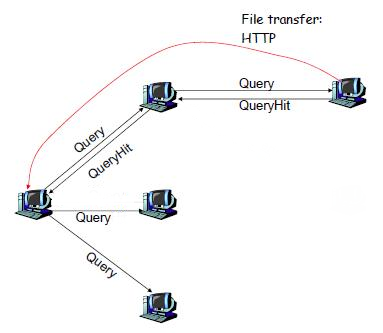
\includegraphics[scale=1.5]{img/gnutella-flood.png}
\caption{Demonstration of Gnutella's file searching mechanism \cite{gnutella-flood}}
\label{fig:gnutella-flood}
\end{figure}

    Partially centralized architectures were defined as similar to those which are decentralized, but with the added caveat that some peers are chosen to service a portion of the network.
    This is done to take use from the fact that not all network peers are alike in terms of memory, computational power, or other relevant resources.
    As such, more capable peers are elected as "supernodes" and are delegated with more responsibilities, noting that the network self-configures in situations where such elected nodes either fail or willingly leave the network, and as such there is no single point of failure as there would be on a true centralized architecture.

    A hybrid architecture approach in a \gls{p2p} network employs some elements from the client-server architecture.
    With Napster \cite{napster} as an example, whilst peers still operate as servers or clients, they must contact an intermediary and central server when querying for content, which will in turn redirect them to one or many peers that contain it - a similar concept applies for BitTorrent, where such intermediary servers are called trackers.
    Obviously, the choice to add a centralized aspect to the architecture hinders many of the advantages from a purely unstructured solution - namely its scalability, resilience to failure, and decentralization of control - serving as a trade-off to facilitate the control and maintenance of the network, as well as the peers' ability to bootstrap to it and locate content.

    A \gls{p2p} architecture is structured if it employs some non-random and systematic criteria on how the network operates, e.g., how peers organize themselves and where content is stored and how it it retrieved.
    For example, FreeNet \cite{freenet} uses the content's hash as a key that is used to query for it, and which in turn is used by the peers in each subsequent hop to know where to forward the request, instead of flooding the network in attempts to blindly find it like Gnutella does.
    Many of the structured \gls{p2p} architectures rely on \glspl{dht}, which act as a decentralized map structure that binds a given key to some content in the network, in such a way that the full key-space is partitioned over the peers.
    Two examples of structured \gls{p2p} architectures that use \glspl{dht} can be seen in Figure \ref{fig:dht-usage}. Specifically, Figure \ref{fig:chord} displays how the Chord algorithm uses a circular \gls{dht} where each peer knows the location of some peers that are their predecessors, and some that are their successors.
    When a peer needs to query for some content, it uses its key to firstly search for it locally and, if it doesn't exist, it forwards the query to their successors, and the process recursively continues.
    On the other hand, Figure \ref{fig:can} display how \gls{can} has the key-space mapped to a virtual two dimensional grid, and its area is partitioned to peers considering a deterministic function, which in turn is used by querying peers to figure out where a given content is stored.
    A straight arrow from querying node to providing node represents the routing path that the querying message must travel: A-B-E.

    Employing a systematic way to self-organize and share content is the means to guarantee that a \gls{p2p} network can be fully decentralized whilst maintaining a desirable level of performance.
    However, the reliance on structure means that it must be maintained, e.g., managing neighbour pointers on Chord or managing area allocations on CAN, and that can be costly or even impossible with high rates of peer churn, i.e., with a sufficiently large rate of peers entering and leaving the network.

\begin{figure}[t!h]
    \centering
    \begin{subfigure}[t]{0.4\textwidth}
    \centering
    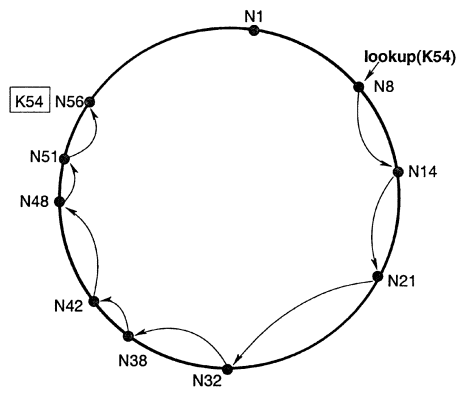
\includegraphics[width=5cm]{img/chord-lookup.png}
    \caption{Chord file query mechanism \cite{stoica2003}}    
    \label{fig:chord}
    \end{subfigure}
    ~
    \begin{subfigure}[t]{0.4\textwidth}
    \centering
    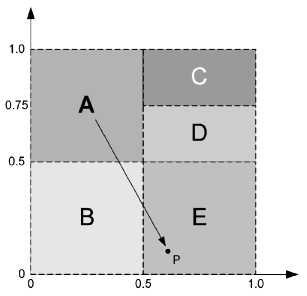
\includegraphics[width=5cm]{img/can-lookup.png}
    \caption{CAN file query mechanisms \cite{p2p-survey-1}}
    \label{fig:can} 
    \end{subfigure}

\caption{Examples of structured P2P query mechanisms that utilize DHTs}
\label{fig:dht-usage}
\end{figure}

\subsection{Effects to the Network Infrastructure}

\label{ssec:p2p-effects}

    Historically, \glspl{isp} have deemed \gls{p2p} traffic as unideal or even undesirable.
    Besides the aforementioned illegality precedent that is tied to \gls{p2p} applications, the overall properties of \gls{p2p} networks make them unappealing to support - due to the distributed nature of these types of networks, the overall traffic is less predictable, with the higher upload traffic volume in edge networks requiring infrastructural investments, and the network-agnostic operation mode of \gls{p2p} applications leads to inefficient and uncooperative network resource usage.

    \gls{p2p} networks who neither have structure nor a central point of control have to utilize content retrieval methods which are bound to be less efficient than their counterparts.
    However, architectures which fit in these categories mostly do so with a clear purpose - Gnutella's decentralized nature makes it very hard for individual nodes or external entities to regulate what can happen in the network (such as enforce legal actions), and its lack of structure simplifies the implementation and reduces the overall effort to bootstrap to the overlay, making it a good fit for applications with a high peer churn rate.
    Similarly, FreeHaven, an also unstructured and decentralized \gls{p2p} protocol, has its architectural decisions fit a very specific use case, as it "emphasizes distributed, reliable, and anonymous storage over efficient retrieval" \cite{freehaven}.
    The lack of systematic means to efficiently locate content by these \gls{p2p} architectures means that more ad-hoc methods have to be used, which are less efficient and thus incur in bigger workloads for \glspl{isp} - the usage of query flooding by Gnutella and message broadcasting by FreeHaven are examples of this.

    The usage of structure by \gls{p2p} networks can, as stated before, result in more efficient content and peer location algorithms.
    However, maintaining such structure also requires a chunk of \gls{isp} resources, as peers need to periodically update other neighbouring peers, as well as react them abruptly entering and leaving the overlay.
    The usage of key-value mappings with \glspl{dht} can also have the potential to be \gls{isp} unfriendly, as the hash function can be designed to evenly distribute resources over the peer pool, and thus over the network - whilst such property is certainly advantageous in certain use cases, doing so removes any application context that exists in the content - for example, grouping resources which belong to the same web page with such a method isn't efficient, as they will be individually hashed and spread throughout the network, despite the fact that they'll likely be requested together for each page access.

    A first point of improvement is optimizations made in the applications themselves to less degrade network resources.
    An example of these can be visualized in Figure \ref{fig:p2p-optimization}.
    Specifically, regarding Figure \ref{fig:chord2}, a point of optimization in the Chord system would try to reduce the number of query messages per resource by increasing the number of successors a given node knows.
    That way, the querying node can instead query not for the single successor it knows, but instead by querying for the one who's ID immediately precedes the content's, thus insuring a reduced number of hops to retrieve the message.
    This consequentially also reduces the total amount of traffic on the network, and improves application times.
    Regarding Gnutella in Figure \ref{fig:gnutella2}, a point of optimization would try to tackle the usage of query flooding to locate data, as such flooding grows exponentially and thus intakes a massive toll on network resources.
    A query flooding system would not be as prejudicial if content was equally scattered throughout the overlay and each given content was a minimal amount of hops away.
    However, as concluded by extensive analysis of user traffic on Gnutella during its heightened use, nearly 70\% of users shared no files and nearly 50\% of all responses were returned by the top 1\% of sharing hosts \cite{freeriding-gnutella}.

\begin{figure}[t!h]
    \centering
    \begin{subfigure}[t]{0.4\textwidth}
    \centering
    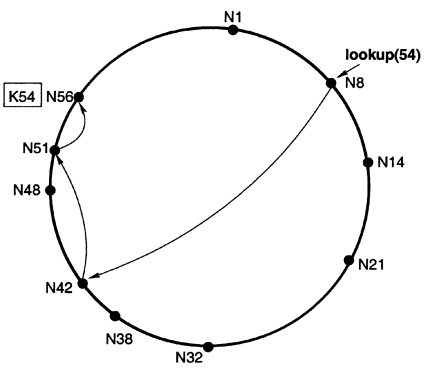
\includegraphics[width=6cm]{img/chord-lookup-efficient.png}
    \caption{Chord file query mechanism with more neighbours known per peer \cite{stoica2003}}
    \label{fig:chord2}
    \end{subfigure}
    ~
    \begin{subfigure}[t]{0.4\textwidth}
    \centering
    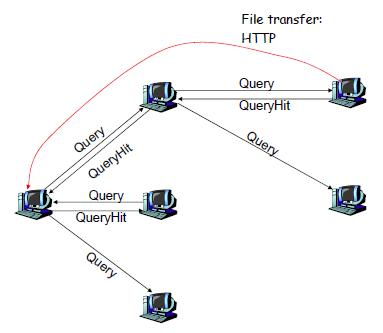
\includegraphics[witdh=6cm]{img/gnutella-flood-efficient.png}
    \caption{Gnutella file query mechanism assuming reduced resource-to-peer hop distance}
    \label{fig:gnutella2}
    \end{subfigure}
    
\caption{Examples of \gls{p2p} query mechanisms when application optimizations are in place}
\label{fig:p2p-optimization}
\end{figure}

    Regardless of the many ways through which \gls{p2p} systems can operate, e.g., in regards to structural mechanisms and centralization, and even disregarding potential application optimizations, no classic \gls{p2p} system operates in full understanding of the underlying network topology, nor with a cooperative behavior towards \glspl{isp}.
    The network-agnostic manner under which they operate results in overlay networks which are layered on top of the underlay where they run, as exemplified in Figure \ref{fig:overlay-underlay} - as \gls{p2p} applications are network-agnostic, two neighboring peers could exist in completely different contexts on the common network layer - for example, they could either be connected by a single data link or be multiple network provider domains away from each other.

\begin{figure}[!h]
\centering
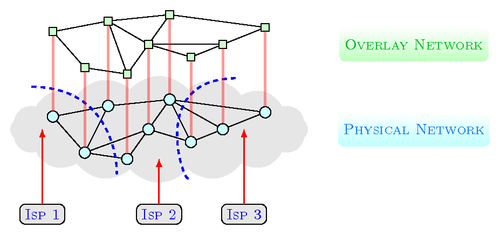
\includegraphics[scale=3.0]{img/p2p-topology.png}
\caption{Example demonstration of an overlay network and corresponding physical layer \cite{overlay-vs-underlay}}
\label{fig:overlay-underlay}
\end{figure}

    The inability of \gls{p2p} applications to localize traffic is seen as a big problem - as concluded by \cite{liao2014}, \glspl{isp} face bottleneck bandwidth pressure in the large scale Internet of the future, with it being in particular from \gls{p2p} applications.
    However, an argument is made that an increase in users from such applications is not necessarily harmful, and perhaps helpful, if traffic locality can be boosted.
    Thus, there is a necessity to ensuring that peers prefer to generate traffic within network locality over traffic that crosses network borders.

    A first step towards more traffic locality would be increasing the availability of content inside network boundaries, through means such as cache injections or peer content serving incentives.
    Given that content resides locally, a second step would be that \gls{p2p} applications have a network-aware vision of the overlay, which does not happen with classic \gls{p2p} protocols.
    This issue is particularly damaging in \gls{p2p} applications whenever neighbours are selected, and whenever a service exists redundantly in the network and a decision must be made in regards to what peer or collection of peers to consume the service from.

    If it is the case that \gls{p2p} applications are not locality aware, it can easily be seen how this can be an issue. In one hand, for the applications, choosing peers which are not local to the querying peer may result in more time to retrieve the requested contents. 
    In the other hand, for the \glspl{isp}, bad network resource utilization can incur in higher operational costs, and may degrade overall network performance in many cases, e.g., by not being able to stop applications from overusing inter-AS links, which usually are network bottlenecks (a conventional wisdom demonstrated in \cite{akella}) and which, due to peering agreements with other \glspl{isp}, are less desirable to be overused due to peering costs.
    If the \gls{p2p} application were to attempt to choose the peers that would most effectively serve the querying peer, it could depend on privileged information that the ISP has on the network's properties and current status, such as the inherent network topology, link properties, or scheduled server maintenance.

    Attempting to optimize peer selection without a co-operational channel with \glspl{isp} would be sub-optimal, as not enough information can be derived with proving alone, and could perhaps even be more damaging with the wrong techniques - consider a peer selection algorithm that chooses the peers with lowest \gls{rtt} of a probing ping message, whilst having no indication on available end-to-end bandwidth, existing network bottlenecks, or peak traffic hours.
    Likewise, attributing neighbour pairings via geographical proximity, whilst initially seems like a good step in location awareness, may also not be optimal - \glspl{isp} may not always prefer geographical proximity in connections, as peers could be very geographically close but residing in different \glspl{as} and thus separated by costly links.
    Other peer-selection techniques focus on randomly selecting nodes, such as the means through which a BitTorrent tracker selects between redundant peers serving the same file chunk \cite{bittorrent-details}, which is simple and resilient to peer churn \cite{qin2009}, but as a consequence is sub-optimal on network resource usage as no network consideration exists.
    It is reasonable to assert that no \gls{p2p} application can act with full \gls{isp} consideration without directly cooperating with it, and simple heuristics should be, whenever possible, traded for methods where full cooperation with the underlay is done - that is, if the needs of both layers are being met.

    Indeed, it is the case that current \gls{p2p} solutions are \gls{isp}-unfriendly.
    More concretely, \cite{isp-p2p-tussle} shares the view that \gls{p2p} applications and \glspl{isp} are in a tussle, since \gls{p2p} applications generate traffic which favours the application's needs whilst ignoring the \gls{isp}'s, which in turn upsets the latter's business model.
    To name a few examples, BitTorrent seems to employ peer selection algorithms which do not consider the underlay network, which can result in degraded download performance and increased load on \glspl{isp} \cite{qin2009}.
    \cite{karagiannis} found that since this protocol is locality unaware, 70-90\% of existing local content was found to be downloaded from external peers, and suggests that locality-aware content distribution algorithms could significantly reduce the total amount of traffic generated.
    Likewise, Gnutella generates traffic which is not ideal, as it may have to cross ISP network boundaries multiple times \cite{estimating-gnutella} due to the same fundamental issue stated before - an application layer that operates in disregard to the network underlay it runs on.

    As \cite{dan-Commag10} describes, the ongoing friction between the overlay and underlay layers has made it to the point where \glspl{isp} have chosen to throttle the bandwidth of \gls{p2p} traffic, or even outright block it.
    In return, \gls{p2p} applications have tried to mask their presence to bypass such restrictions via tunnelling or using non-standard and random port numbers.
    This is an unsustainable system that is bound to hurt both \gls{isp} profit and application functionality, and a strategy of cooperation between the overlay and underlay layers is crucial to guarantee that the requirements of both parties are met, specially in the face of the increased technical and scale-related challenges of the future.

\section{Content Distribution Networks (CDNs)}

\label{sec:state-cdn}

\subsection{Concepts and applications}

\label{ssec:cdn-concepts}

   A \gls{cdn}, as the name implies, is a network specifically designed with its main focus on distributing content to a set of end users.
   Its design allows for the alleviation of performance bottlenecks on the Internet generated by client requests, and has been recently been considered a powerful tool as a response to the existing high demand for media content, which has a huge share of the global Internet traffic of today.

   Functionalities of \glspl{cdn} include \cite{cdn-survey}:

    \begin{itemize}
        \item \textbf{Content outsourcing and distribution:} Replicate content throughout the network into edge servers, which are deployed nearby end users.
            This allows \gls{cdn} clients to pay for their content to be hosted on these edge servers, and in doing so guaranteeing that it is quickly accessible by end users.
        \item \textbf{Request redirection:} Direct a content request to the most appropriate edge server at a given time.
            This redirection is done considering relevant network properties, such as geographical locations and current server loads.
        \item \textbf{Content negotiation} Manage the network's properties to fit the needs of its clients through negotiation.
        \item \textbf{Management:} Manage the distribution network, which includes accounting, monitoring, statistical analysis on content consumption, etc.
            A close management of the distribution network is important for its business model, as, besides being needed for a billing system, allows for a better understanding of the networks' usage patterns, which is helpful information for better engineering the system to most optimally serve content with increased revenue and decreased costs.
    \end{itemize}

    The current focus of \glspl{cdn} is thus to provide content, e.g., web pages, documents, photos, videos, or media-related streams, with high availability and performance.
    The strategy used by them to guarantee a satisfying \gls{qoe} on a global scale is the deployment of content close to the end-user - a \gls{cdn} contains many nodes which are geographically spread throughout the globe and close to the users they wish to serve, and whenever such users request for content, they are routed to the node which is closest to them (\cite{cookbook}).
    Data replication to servers which are strategically placed closest to end-users, coupled with good means to properly redirect such users to the most attractive edge server, is what allows content to be available more often and more quickly.
    These are undoubtedly attractive features in the world of e-commerce, where user \gls{qoe} can dictate much of the profit - for example, Akamai, one of the leaders in \gls{cdn}-related services, ran a research concluding, among other things (\cite{akamai}):

\begin{itemize}
    \item A 100 millisecond slower web page loading speed can result with a 7\% drop in sales
    \item A 2 seconds slower web page loading speed can almost double the number of visitors who end up abandoning their carts
    \item 53\% of users who use smartphones to visit web stores won't make the sale if the web page takes more than 3 seconds to fully load
    \item 28\% of users won't return to the same web store if they think it takes too long to load
    \item A 250 millisecond faster loading time proved to keep users from visiting a competitor web store
\end{itemize}{}

    It should then come as no surprise that streaming services such as Netflix \cite{netflix} and Youtube \cite{youtube}, who now reach a global scale and whose utility is highly dependant on their high availability and low transmission delay, routinely use \gls{cdn} solutions.
    More broadly, typical \gls{cdn} customers include media and Internet advertisement companies, data centers, \glspl{isp}, online music retailers, mobile operators, etc \cite{cdn-survey}.
    Indeed, companies that wish to provide a given service in the web at scale routinely partner with companies whose focus is providing content delivery services, with popular examples being Akamai, CloudFlare \cite{cloudflare}, or Amazon Cloudfront \cite{cloudfront}.
    Coupled with the promise of highly available and quick content retrieval, these companies also provide other attractive services, such as firewalls and \gls{dos} protection.

    The Internet's currently most targeted use being media consumption has made it so \glspl{cdn} and their providers have an important role in dictating a very considerable percentage of flow of traffic in \gls{isp}-owned infrastructures, and as such their study and improvement is quite important.
    With their great influence over global traffic, active efforts should exist to increase harmonious behaviours between applications that utilize their services and the \glspl{isp}, with the goal in mind being network resource efficiency to guarantee that the infrastructure can remain operational and applications can provide a satisfiable user experience.

\subsection{Architecture}

\label{ssec:cdn-architecture}

    Figure \ref{fig:cdn-conceptual-architecture} represents a high-level conceptual architecture of a \gls{cdn}.
    The true power of a \gls{cdn} comes from its strategically deployed cluster of replicated servers - at a global scale, this implies having them geographically dispersed and located inside or nearby networks with large content demand.
    The origin server possesses the content that is to be served, and the bootstrapping process has it uploaded into the network, which is afterwards replicated into these edge servers.

\begin{figure}[!h]
\centering
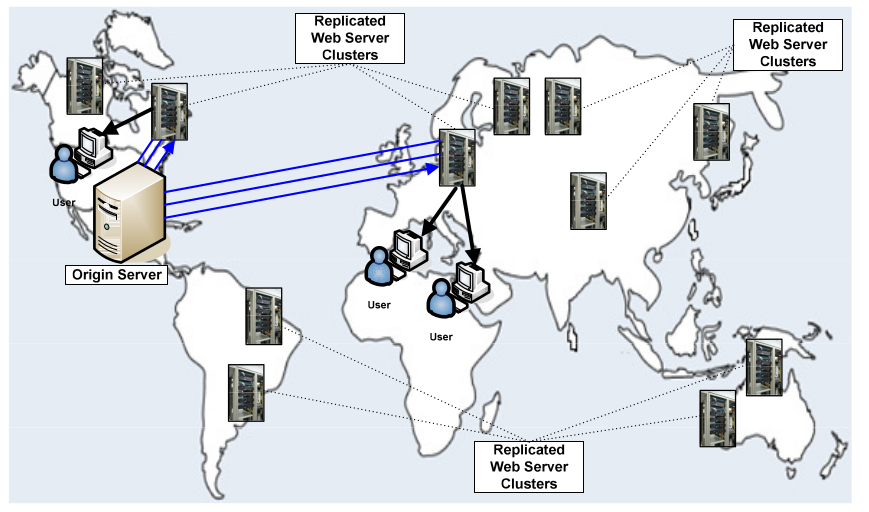
\includegraphics[scale=0.65]{img/cdn-architecture.png}
\caption{Conceptual architecture of a \gls{cdn} \cite{cdn-survey}}
\label{fig:cdn-conceptual-architecture}
\end{figure}

    Figure \ref{fig:cdn-request-routing} displays how, conceptually, the request routing functionality of a \gls{cdn}.
    As can be seen, the request is firstly directed to the origin server, and serves only light, basic content.
    In the situation where large static content is requested, the origin server redirects the request to the \gls{cdn} provider, which utilizes a selection algorithm to elect the most appropriate edge server to serve the content to the end user.

\begin{figure}[ht]
\centering
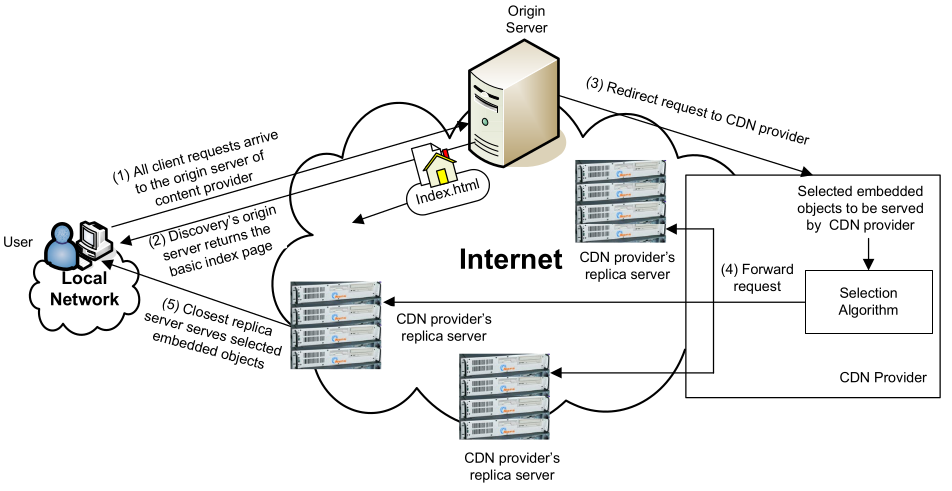
\includegraphics[scale=0.5]{img/cdn-request-routing.png}
\caption{Request routing functionality of a \gls{cdn} \cite{cdn-survey}}
\label{fig:cdn-request-routing}
\end{figure}

    The request routing mechanism is the one that redirects a given user to a given edge server.
    The prevalent approaches are, according to \cite{wichtlhuber2017}, the following:

\begin{itemize}
    \item \textbf{\gls{dns} request routing}: The user must first resolve a domain name to retrieve a content. The \gls{cdn}'s \gls{dns} processes the request and, utilizing the user's \gls{ip} address, historical measurement information and current server loads, responds with the address of the edge server that seems most fitting to provide such content.
    \item \textbf{\gls{http} request routing}: Content is firstly requested to a nearby proxy server, which in turn answers with an \gls{http} redirect to be resolved by the client in order to find the content.
        The \gls{http} requests can occur in subsequent rounds and can also use \gls{dns} knowledge when the redirection domain must be resolved.
    \item \textbf{Anycast request routing}: The \gls{cdn} provider announces an anycast prefix to the network.
        Whenever a router receives multiple announcements to the same prefix incoming from different locations, it chooses one considering some custom criteria, usually being \gls{as} hop count and \gls{igp} weight.
        Thus, different routers can have a given anycast address mapped to different hosts, meaning the ones that are most suitable for that particular router.
\end{itemize}

    These mechanisms are also discussed in \cite{cdn-survey}, but also add:

\begin{itemize}
    \item \textbf{\gls{gslb}:} Service nodes, consisting of edge servers and \gls{gslb}-enabled web switches, are interconnected in a network.
        Individual nodes possess global awareness of the network, meaning the status of each individual server.
        With edge servers having more information on the health and status of all other candidate edge servers, and the web switches acting as authoritative \gls{dns} servers, the network can enable the support of a global-wide server load balancing mechanism that intakes dynamic server information.
    \item \textbf{\gls{url} rewriting:} The origin server redirects the end user via dynamically altering the host pages' \gls{url} links.
    \item \textbf{\gls{cdn} peering:} An extension of a single \gls{cdn} network to multiple, interconnected \glspl{cdn} which serve content on behalf of others when appropriate.
        This is helpful to extend the domain reachability of a single \gls{cdn}, increase fault tolerance, and ability to achieve better performance with more candidate servers to choose and balance loads from.
\end{itemize}

    It is vital that a \gls{cdn} possesses a clear view of the network performance inside its domain.
    \cite{cdn-survey} lists important metrics which are used to measure \gls{cdn} performance:

    \begin{itemize}
        \item Geographical proximity of end users
        \item Path latency
        \item Path packet loss
        \item Path Bandwidth
        \item Path startup time
        \item Path frame rate
        \item Server load
    \end{itemize}

    Means through which these metrics are retrieved by the network include traffic monitoring of end user to surrogate server communications, and surrogate server feedback retrieval via application requests or measurement probings \cite{cdn-survey} \cite{akamai-report}.

    Having a clear understanding of CDN performance is important for system management in two fronts - firstly, through performance evaluation, by providing the billing and monitoring modules the verification of how the network is faring at its task of caching and delivering content on behalf of clients; secondly, through performance optimization, by providing the logical layer an updated view on network status, serving as contextual input that the system uses to better reason on how to act - for example, in regards to the caching and request routing mechanisms.

\subsection{Effects to the Network Infrastructure}

\label{ssec:cdn-effects}

    As previously discussed, \glspl{cdn} came as a tool to strategically position content on the network in such a way that it can more quickly and more reliably be retrieved by an end-user.
    These \gls{cdn} systems are then inherently a means of optimizing network resource utilization in the application layer, and thus are of great interest for \glspl{isp} and, if done properly, can be very appealing not only to them but also to end-users that use applications leveraging these networks.

    The usage of a single content-providing server - or a limited set of them - which is far away from the content demand, that in turn has a large geographical distribution, is prone to server overloading and path congestion problems if a big enough scale is achieved.
    The usage of data caches is a classic solution to network inefficiency problems, which is used by \glspl{cdn} as a means to replicate content to strategic locations to better serve users, with the added benefit for \glspl{isp} that their network resources are efficiently used, with the ability of reducing the total amount of used bandwidth needed for a service to operate - as data travels a shortened total amount of network hops from data source to points of data demand - and reducing congestion of inter-domain links - as data caches will reside locally and redistribute traffic away from highly shared network links.
    It can thus be stated that the relationship between \glspl{cdn} and \glspl{isp} allows for a win-win scenario because efficient network usage has consequentially better service quality, benefiting service providers and applications, respectively.

    However, \glspl{cdn} seem to lack cohesion with the underlying network infrastructure during normal application operations.
    As stated by Akamai, a leader in \gls{cdn} services, in their report \cite{akamai-report}, the large scale and complexity of the Internet, where it takes well over 650 networks to reach 90\% of all access traffic, adds to it many challenges to the \gls{cdn}'s role of content delivery.
    In particular, whilst good investment seems to exist at the first and last mile of Internet access (website hosting and end users, respectively), there seems to be little economic incentive to invest in the middle mile, composed of peering points shared among networks.
    These peering then become network bottlenecks that are susceptible to increased traffic packet loss and latency, making inter-network communications unreliable, and loose coordination between autonomous networks with internal biases is pointed as a main cause.
    Due to this, even a well provisioned data center will be at the mercy of the various inter-network bottlenecks that may arrive, and performance takes a hit.
    In fact, the paper suggests a clean-slate redesign of the Internet as a potential solution to its many problems - besides the peering point congestion mentioned above, inefficient routing protocols, unreliable networks, inefficient communications protocols, and application limitations also add to the problematic - but such a redesign to a massive and highly invested global infrastructure doesn't seem plausible.

    In alternative to proper network infrastructural insight, \glspl{cdn} have to rely on network probing, traffic monitoring, and server feedback, as discussed on Section \ref{ssec:cdn-architecture}.
    Even assuming that these are sufficient, the usage of probing techniques will incur in overhead traffic on the network, with this overhead being exacerbated if many other overlay networks or applications also apply this technique.
    Similarly, traffic monitoring to extract end-to-end path metrics to end users requires resources and takes time, and may also incur in redundant operations being applied on the network.
Such advantage goes outside of the \gls{cdn} realm, being useful for any overlay-residing application that wants to utilize network probing to be more underlay-aware.

    Advantageous as network probing and traffic monitoring mechanisms can be for \glspl{cdn} to properly conduct request routing and caching decisions, a case must be made for proper application-infrastructure synergy during decision making in the overlay.
    Much like \gls{p2p} systems, to infer on network status by measuring it is insufficient when compared to receiving input from trustworthy and authoritative entities that possess privileged network information, such as \gls{isp} administrators.
    Attributing node pairings entirely on geographical data was previously discussed as being a non-optimal way of assessing node selection at the application layer in Section \ref{ssec:p2p-effects}, and the same would apply in the case of \glspl{cdn}, where edge servers are paired with end-users.
    Again, much like in the scenario of peer selection in \gls{p2p} systems, the usage of network measurements made by the \gls{cdn} itself to better pick the appropriate end-server, while potentially beneficial, can certainly be improved upon if it used additional, hard to retrieve data that only \glspl{isp} or other privileged infrastructural entities could possess, and which are at position to guide applications in the infrastructure they deeply possess knowledge on.

    There indeed seems to be a consequential coupling between overlay decisions in the \gls{cdn} systems and the underlying infrastructure.
    If the \glspl{cdn} were not to take \gls{isp} input when redirecting clients, suboptimal choices would be made that would be prone for bottleneck congestion, and if, in the other hand, \glspl{isp} were to employ only their own biases in content request redirection, user-level application \gls{qos} agreements might not be met.
        \cite{pushing-cdn-isp-collaboration} states that this lack of awareness to network status is indeed problematic for \gls{cdn} systems, listing end-user mismatching to edge servers based on dubious \gls{dns}-based location binning and resource consuming, non exact methods to detect bottlenecks, as well as lack of agility in server deployment in ideal locations.
        This is a view shared by \cite{cdn-isp-cooperations}, which adds that these problems reside in a shared medium that raises the opportunity for cooperative behavior that would enable better application performance and optimized \gls{isp} resource utilization.
    In fact, Akamai themselves have formed content delivery strategic alliances with major \glspl{isp}, with AT\&T \cite{att}, Orange \cite{orange}, Swisscom \cite{swisscom} and KT \cite {kt} among them \cite{pushing-cdn-isp-collaboration}, which hints at this type of partnership being the norm for content distribution technologies.

        \gls{isp} input permits applications to act in a more network-aware fashion than without it - whereas pairing overlay nodes or deploying edge servers in terms of geographic distance, \gls{rtt} distance, or any other metric, may give further decision power than a purely network-agnostic overlay system, proper guidance by \glspl{isp} could help pairing based on more complex metrics that, besides the aforementioned ones, also consider ISP objectives, e.g., to minimize network distance, avoid bottlenecks, locate content caches, etc.
        A more efficient Internet can be obtained if many other overlays coordinate their efforts with the \gls{isp}, which in turn can now orchestrate its traffic in a way that would previously be generated with no prior guidance, and that can now be engineered to maximize network resource utilization and, consequently, application performance.

\section{Client-Server Model}

\label{sec:state-client-server}

\subsection{Concepts and applications}

    The Client-Server model is a classical way of attributing roles in the network.
    Whereas the \gls{p2p} architecture blends server and client roles into each node, this architecture delineates two distinct ones - the client and server - and their purpose on the network, as Figure \ref{fig:cli-serv-architecture} shows.
    With it, the service layer is centralized onto the server nodes and the only role expected of client nodes is to request services from them.
    Operating with opposite philosophies from the \gls{p2p} architecture, it is to be expected that the advantages and disadvantages should too be contrasting - by centralizing the services, maintenance and general administration of serving nodes become attainable, and by limiting the number of servers to a select and trustworthy few, instead of scattering that functionality to all nodes in the network, greatly minimizes security risks.
    On the other hand, the drawbacks are also apparent and mirror a distributed solution - issues of scalability, resilience to failure, and resilience to monopolization of power arise from the decision to engineer an application that creates clear boundaries between client and server.

    \begin{figure}[!h]
    \centering
    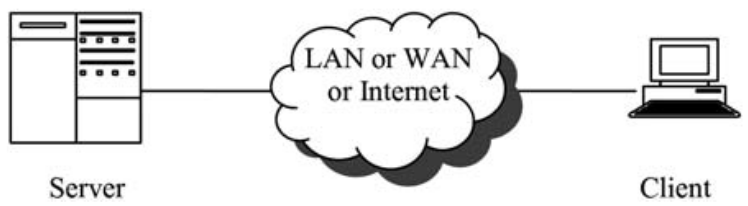
\includegraphics[scale=0.55]{cli-serv-architecture.png}
    \caption{Client-Server architecture \cite{cliserv-p2p}}
    \label{fig:cli-serv-architecture}
    \end{figure}

    This classic architecture has seen a lot of adoption by applications, with use cases that include serving content via \gls{http} or \gls{ftp}, or enabling e-mail communications \cite{cliserv-p2p}, to name a few.
    Adding to this, the client-server approach also serves as a direct alternative to the \gls{p2p} one in many fields, e.g., file transfer or media streaming, with their respective advantages and disadvantages needing to be weighted out for a proper choice to be made.

    As an attempt by service providers to still operate a client-server model whilst reducing its associated downsides, given techniques were created and employed.
    One of which, by the name of \gls{cdn}, is of particular importance in this work and as such has its specific overview in Section \ref{ssec:cdns}.
    Some others will be discussed below.

    Server mirroring, one famous technique, is the act of continuously synchronizing a server into its replica, or mirror, essentially creating an exact copy of it that is now accessible as if it were the original.
    Whilst \glspl{cdn} aim at replicating chunks of contents wherever it may be necessary, the act of server mirroring performs an integral copy of a server which is self sufficient at servicing a given client, as long as it periodically checks up with the primary server for synchronization.
   It is a standard business strategy that uses redundancy as a means to increase reliability, availability and performance.
   The existence of many servers that perform the same task means that these can be strategically chosen to serve a client in a given situation, e.g., by selecting the one that has reduced load and smaller end-to-end message delay to the user.
   Figure \ref{fig:mint-mirrors} shows an application of this, where multiple server mirrors exist to deliver software packages to the Linux Mint \cite{linux-mint} distribution.
   The user has the choice to manually select one of these mirrors, and ideally chooses the one that is most fitting to them.

    \begin{figure}[H]
    \centering
    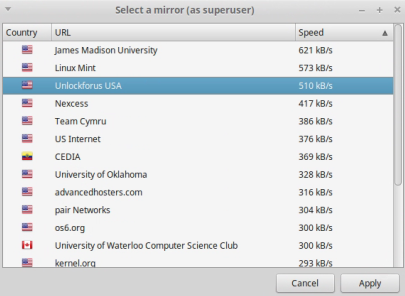
\includegraphics[scale=0.8]{mint-mirror.png}
    \caption{Linux Mint prompt to select a software repository mirror}
    \label{fig:mint-mirrors}
    \end{figure}

    Server load balancing is another popular technique to reduce server-client downsides, and it refers to the act of distributing tasks over a set of computing nodes as a means to make the service more efficient, since a server with little processing load is bound to respond quicker than one with more, and situations of overloading become less common as it is now spread out over multiple processing units.
    Load balancing algorithms can be categorized, according to \cite{load-balancing}, in two categories:

    \begin{itemize}
        \item \textbf{Static}: Does not take current system status into account, instead acting upon static rules that define the load type, in regards to, for example, processing power and memory requirements.
            A round-robin or random approach of load attribution are part of a static approach.
        \item \textbf{Dynamic}: Load is distributed at run time, considering dynamic information about the system that is continuously being collected.
    \end{itemize}

    A static approach can be compelling due to its simple nature that makes it easy to implement and much faster in comparison to run.
    On the other hand, a dynamic approach is more complex by definition as it requires the additional infrastructure required to collect and compute upon the system statistics.
    As it might be expected though, a load balancing scheme that attempts to optimize resource utilization considering real-time information about system status and performance is bound to have bigger potential at effectively selecting which server should handle a given request since more factors are known to better aid the decision, including the current server loads in the server cluster, their available resources, network conditions, etc.

    Several methods exist through which to implement load balancing.
    For example, \gls{dns}-based approaches perform the load balancing at the name resolving stage, where the IP address response is given after selecting an optimal server, such as the proposal in \cite{dns-load-balancing}.
    \gls{sdn} solutions, as another example, leverage a control pane that is responsible for intercepting server access calls and activate the load balancing mechanisms that redirect to the selected server, as happens in the proposal in \cite{sdn-load-balancing}.


\subsection{Effects to network infrastructure}

    As a base method, the utilization of the client-server architecture is not at all recent to \glspl{isp}.
    Quite the contrary, it is the norm throughout the decades to provide a service by using a set of single-purpose server machines.
    Intuitively, using a limited number of servers to respond to clients needs will have problem scaling, as increased demand will overload servers and create path congestion, hence the need to employ some of the strategies discussed above.
    These strategies come from the necessity to fulfill both application and \gls{isp} requirements, i.e., to achieve proper \gls{qos} levels and infrastructure resourcefulness that helps the general good function of the network, respectively.

    Much like the content replication utilized in \glspl{cdn}, an integral replication of a main server proves itself as an advantageous tool capable of delivering services more closely to users, and as such allows the reduction of total amount of bandwidth used to serve all clients.
    Optimizing application traffic is crucial to guarantee good network resource usage, and in case of server mirroring it comes down to good strategical deployment and dynamic, intelligent algorithms to properly attribute mirrors to requesting end-users.
    Giving end-users the choice to manually select the serving mirror, as commonly happens when downloading software, for example, seems problematic, as application-generated traffic is not optimized.
    In fact, when considering the Linux Mint software package distribution discussed above, despite there currently existing seventy mirrors deployed throughout the globe to fit this role, a large number of these remains mostly unused whilst the main and default server is constantly prone to overworking \cite{mint-article}.
    It can be stated that end-users both don't care enough to optimize traffic nor do they have enough information to properly do so even if they did.
    Deployment of server mirrors is a great tool that brings with it the issue of optimizing server selection, and much like all examples given so far, traffic generated by applications can be firstly optimized by the applications themselves if they consider static and dynamic information of the network they operate on.

    Load balancing is too a point of great interest in the task of application-layer traffic optimization.
    The task of attributing a current request to a pool of available redundancy workers is a common strategy to help scalability, and how it is done has concrete network consequences as it has the power to shape great amounts of traffic in ways that can be more or less preferable for \glspl{isp}.
    It could then be deduced that a load balancing strategy has better chances of being efficient if it fully aware of both server status and network conditions.
    Doing so with \gls{isp} cooperation would reveal insight in some network status information and preferences that could not be retrieved otherwise, and, much like what was argued for in section \ref{ssec:cdn-effects}, could severely reduce overhead traffic created by probing and measurement strategies if such data was centralized in an entity with full network knowledge.

\section{Traffic optimization by applications and layer-cooperative approaches}

\label{sec:state-solutions}

    This section serves to display proposed solutions and existing implementations that have been made in the attempt to optimize application traffic utilizing network information.
    Given the increasing scale of the Internet as a near ubiquitous system, and the increasing tension between applications and service providers, it comes with no surprise that the area of layer cooperation has been through exhaustive work.
    Many solutions have been devised for specific use cases, with varying degrees of power given to each one of the layers, and different levels of cooperation.
    Along with their description, their review is made in regards to what the proposals state their impact is to applications and the infrastructure, as well as the accompanied advantages and disadvantages.

\subsection{Peer-to-peer applications}

\label{ssec:approaches-p2p}

    Many different mechanisms have been developed with the goal of decreasing tensions between \glspl{isp} and \gls{p2p} applications, which is a subset of the general layer cooperation problem.
    Figure \ref{fig:p2p-isp-interactions} represents a grouping proposed by \cite{dan-Commag10} where such mechanisms are ordered in agreement with how much involvement the \gls{p2p} systems and the \glspl{isp} have. 

    \begin{figure}[H]
    \centering
    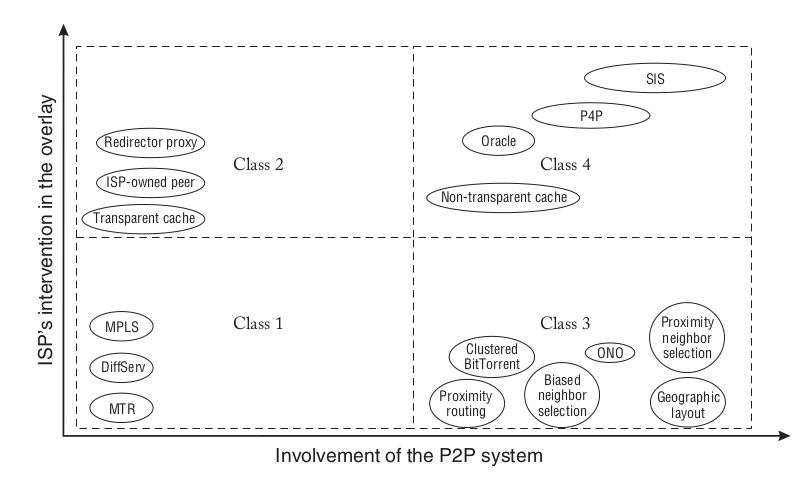
\includegraphics[scale=0.65]{img/approaches-isp-p2p.png}
    \caption{Approaches to decrease tension between \gls{p2p} applications and \glspl{isp} grouped by their involvement \cite{dan-Commag10}}
    \label{fig:p2p-isp-interactions}
    \end{figure}

    In a more detailed fashion, these classes are as follows:

    \begin{itemize}
        \item \textbf{Class 1}:
            There is not much - or any - interference in the overlay by \glspl{isp} nor are \gls{p2p} systems cooperative.
            Instead, \glspl{isp} apply traffic engineering methods to selectively favour types of traffic.
            This is usually done to guarantee certain \gls{qos} levels to some classes of traffic, which are then to be treated favourably at the forwarding and routing levels.
            Examples of such techniques are \gls{diffserv}, \gls{mtr} and \gls{mpls}.
            These classes of methods do not fix the underlying application behaviour, but are instead used to control preexisting traffic.
            As such, the peers' routing decisions are not affected and \gls{p2p} traffic still remains non localized.
        \item \textbf{Class 2}:
            There is \gls{isp} intervention in the overlay in such a way that peers continue normal operation without realizing that such interventions occur.
            This can be reached via the use of proxies that can affect the control plane with the redirection of content requests to local peers, or at the data plane with content caches which act as normal peers and are strategically placed in the network.
            These methods are advantageous because they do not require any changes to the \gls{p2p} protocols, because the \gls{isp} has an active role in molding to the overlay, intercept traffic, and either help or guide it in a way that favours them.
            Indeed, these techniques haven been proven to work , as concluded in \cite{dan-Commag10}, and put into practice, for example, in \cite{programmable-trackers}, \cite{configurable-trackers}, and \cite{rev3}, via the specification of a BitTorrent tracker that is programmable to allow for \gls{p2p} qualitative differentiation and \gls{isp}-cooperative traffic engineering that could help reduce inter-domain traffic significantly.
            Additionally, in \cite{altruistic-gnutella}, with the injection of special nodes on the Gnutella overlay which interface with the base protocol nodes but with the added caching and load-balancing mechanisms, in the attempts to alleviate the great amount of "free riding" that exists in Gnutella applications - as discussed in Section \ref{ssec:p2p-effects} - by minimizing the total amount of query floods and more evenly distributing content throughout the network for increased infrastructure resourcefulness.
            However, this class of mechanisms is not without its challenges - firstly, it involves much effort by \glspl{isp}, as it requires structural upgrades and constant adaptiveness to new and changing \gls{p2p} protocols.
            Perhaps worse, even when considering proper budget and maintenance, such methods can prove themselves to be not possible at all - for legal reasons, as data caches could possibly contain illegal content; and for technical reasons, since the packet inspection required by \glspl{isp} to detect and steer \gls{p2p} traffic may be blocked due to the peer's attempts to mask its traffic.
            It's also important to note that since no application-layer input exists, this approach could be one-sided in the sense that only \gls{isp} needs are favored without directly considering application needs.

        \item \textbf{Class 3}:
            Relative to previous classes, the active role is switched and it is the \gls{p2p} system itself that acts in regards to the underlay it operates on, but without \gls{isp} involvement.
            Peers probe the neighboring network elements as a way to get more familiar with connection properties, and act on these probings during operation, e.g., when choosing neighbours to construct the overlay network with, or when choosing from whom to request a given resource.
            Whilst these methods can be advantageous for both applications and \glspl{isp}, it can't be assumed that to always be the case - as peers have no \gls{isp} input, they cannot have a full knowledge scope of the network and its needs, and as such these application optimizations can end up being more hurtful than helpful.
            For example, consider a scenario where a peer uses \gls{rtt} measurements to choose between two candidate peers, but the one that is geographically closest to it belongs to another \gls{as}, and his preference for it to supply the service would incur in more infrastructural costs.
            The paper describes this class as a "win-not-lose" situation, meaning that while the \gls{p2p} system can, in the right circumstances, improve their performance via measurement-oriented strategies, the ability to act in a way that positively affects the underlay, without any feedback from \glspl{isp}, cannot be guaranteed.
            Such an example of class 3 mechanisms could be seen in \cite{qin2009}, which improved BitTorrent's download performance and even managed to reduce \glspl{isp}' backbone and cross-\gls{isp} traffic.
            The technique consisted of having peers send traceroute measurements to the tracker, which in turn grouped the peers into local, intra-\gls{isp} and inter-\gls{isp} groups, with the assumption that inter-\gls{isp} links generally have much more latency than the rest.
            As peers would later query the tracker for content, the returned peer list would be biased in such a way that promotes traffic locality.
            Another example of this is \cite{kim2011}, which devised a \gls{cdn}-\gls{p2p} hybrid where peers utilize \gls{rtt} measurements to group themselves by separate orders of geographical proximity with the same intent of the previous example, which is to localize traffic whenever possible.
            This technique also proved itself to be advantageous, as the solution was more efficient in terms of reduced total service disruption time when compared to a previous iteration of the hybrid architecture which used random peer selection to look up available target peers.
            As a final example, \cite{topology-aware-p2p-server-selection} proposed a node binning scheme that groups nodes of similar orders of magnitude of \gls{rtt} values to pre-defined landmarks, and utilized such scheme for topology-aware overlay construction mechanisms in some unstructured and structured \gls{p2p} overlays.
            Results allowed to conclude that even surface-levels topological information is advantageous and can significantly improve application performance.

        \item \textbf{Class 4}:
            Full and active cooperation exists between the \glspl{isp} and \gls{p2p} systems.
            The role of the \glspl{isp} is to provide information and guidance, and \gls{p2p} systems let themselves be influenced during operation.
            It is the methodology that most comes close to a mutually advantageous scenario for both parties, given that they both keep the entire group's needs in mind.
            For example, \cite{locality-aware-p2p} proposes an oracle that receives as input a list of candidate peers that the querying peer is considering connecting to, and ranks them by client connection proximity.
            Such method was tested in a simulated environment and proven to decrease negotiation traffic and improve scalability of \gls{p2p} networks.
            Similarly, \cite{configurable-trackers} proposes a framework for programmable trackers in a BitTorrent scenario, providing an interface to directly define tracker behavior which, given ISP input, can provide a collaborative environment between infrastructure administrators and the BitTorrent users in an attempt to, among other things, localize traffic.
            The functional intent of the oracle pattern is that he possesses privileged network information and acts on it to provide guidance to querying applications, and thus has the power to impose policies and optimizations unto applications, e.g., pair peers which are the least number of network hops apart via a Dijkstra algorithm using link costs derived from network-related ISP insight.
            Another approach that could be used by the oracle proposed in \cite{han2009} contains algorithms to dictate peer selection, task assignment and rate allocation.
            The method requires the full network topology as input - including link capacities and peer service costs - to minimize file downloading time and cost.
            The oracle would also be free to enforce \gls{isp} biases as its preferences by modifying such algorithms to, for example, minimize usage of costly links (such as inter-\gls{as} ones, and subject to peering agreements).
            The \gls{alto} working group - whose work this thesis attempts to materialize into a working system and further extend its features - was formed to standardize the oracle-user scenario so it could be properly used in many situations at the scale of the Internet.

    \end{itemize}

\subsection{Content Distribution Networks}

\label{ssec:cdns}

    Given the current share that \glspl{cdn} have on global Internet traffic of today, coupled with the demand for a good \gls{qoe} by end-users, it should come as no surprise that this application domain has also been through efforts to optimize its traffic.
    One such way to do so is to optimize client query redirection, i.e., better choose which edge server should be attributed to an end-user when a name resolution is requested for some content.

    \cite{gromov2014} considers a \gls{cdn} built to deliver video data where some given set of content exists redundantly in many edge-servers, and presents an algorithm where the choice is made to optimize client download time, which in turn has to consider the network parameters at time of request, as well as current server load.

    Some simple, flexible and scalable techniques exist that utilize no ISP input.
    For example, \cite{topology-aware-p2p-server-selection}, mentioned in Section \ref{ssec:approaches-p2p} for its \gls{p2p} overlay construction with a binning technique based on \gls{rtt} measurements to landmarks, also utilized such binning technique for improved server selection.
    Similarly, \gls{ietf} tackled application traffic optimization via multi-\gls{cdn} cooperation, and devised a problem statement in regards to \gls{cdni} \cite{cdni-problem-statement}, which outlines the efforts required to specify a set of interfaces that allow for the interconnections of many \glspl{cdn}, with the added benefits that a multi-\gls{cdn} system, over an individualistic one, will have better properties, e.g., in regards to availability, coverage, and supported capabilities, as well as better \gls{qoe} for the end user, and reduced delivery costs for the service providers.
    The four devised interfaces - \gls{cdni} Control interface, \gls{cdni} Request Routing interface, \gls{cdni} Metadata interface, and \gls{cdni} Logging interface - are all to be operated at the application layer, and the group states that no new application protocol needs to be devised.
    Instead, existing protocols could be leveraged, e.g., \gls{http}, Atom publishing protocol, \gls{xmpp}, and in particular to the \gls{cdni} Request Routing interface, the \gls{alto} protocol could enable \gls{cdn} server footprint retrieval.

    Centralized network measurement repositories for wide consumption were tackled in project such as \gls{idmaps} \cite{idmaps} and \gls{gnp} \cite{gnp}, that describe architectures for a global distance estimation service, leveraging measurements made by specialized nodes that retrieve raw network data, and heuristic provide scalable and functionally reliable path costs in metric such as bandwidth and latency.
    These consist of systems that centralize and share network probing results to querying entities, thus minimizing overhead traffic on the network.
    Such advantage goes outside of the \gls{cdn} realm, being useful for any overlay-residing application that wants to utilize network probing to be more underlay-aware for application optimization.

    \cite{cdn-isp-cooperations} argues for the advantage of \gls{cdn}-\gls{isp} cooperative interactions and overviews three possible strategies that will be now discussed briefly: \gls{padis} \cite{pfa-10} is a system deployed and controlled by \glspl{isp} that monitors the network by listening to \gls{egp} and \gls{igp} messages and contains a privileged view of the topology and its status.
    It provides a service that ranks host-client pairs in regards to, for example, delay, bandwidth, or hop count, and experimental testings concluded that the download times of content provided by \glspl{cdn} that utilize \gls{padis} could be improved up to a factor of four, and generally gives much flexibility for \glspl{isp} to engineer traffic; \gls{cate}  \cite{fps-12} is designed in a similar manner to \gls{padis} but requires no client-side configuration, and experimental results concluded that network wide traffic was reduced by 15\%, link utilization was reduced by 40\%, and user-server performance generally increased; \gls{netpaas} \cite{pushing-cdn-isp-collaboration} was devised to fulfill two key enablers in a fruitful \gls{cdn}-\gls{isp} collaboration - user-server assignment, as it was tackled in the previous two examples, and server allocation, i.e., where should a \gls{cdn} deploy its servers and its contents.
    This service, besides having the advantages of increased application performance and better \gls{isp} traffic control that were also mentioned in the previous two solutions, also facilitates the task of server allocation for \glspl{cdn}, reinforcing the discussed advantages and optimizing \gls{cdn} operations.
    Still in the topic of \gls{cdn}'s edge server selection, \cite{wichtlhuber2017} suggests an \gls{sdn}-oriented solution that combines the performance of \gls{dns} load balancing with the low management overhead of \gls{ip} anycast.
    Load balancing is performed at the \gls{sdn} control layer by applying collaborative efforts between the \gls{cdn} and the \gls{isp}.
    This example of layer cooperation can allow for many optimization opportunities that leverage an existing and low-maintenance mean of request routing with the flexibility of \gls{sdn} solutions.

\subsection{Server-client applications}

    Attempting to optimize web server selection, \cite{kenichi} argues that \gls{dns}-oriented solutions, which select the nearest server but also employing load balancing, may not be the best at optimizing server-client \gls{qos} levels.
    Instead, it proposes a selection based on \gls{qos} measurements, from which three types are distinguished: a static method, such as choices based on least number of hops to server (which is unlikely to change); a dynamic method, consisting of network probing to assert, for example, \gls{rtt} values to the servers; and statistical methods, which decide based on a larger set of measurements previously made in various points in time.
    Utilizing the latter method, \gls{rtt} measurements and web-related request benchmarking is made, such as time to establish a \gls{tcp} connection, elapsed time from an \gls{http} GET method to first packet received, time to retrieve data fully, etc, every five minutes and spanning several weeks.
    The work concluded that statistical methods used to select between multiple equal web servers had high correlation with download time from the selected server, but optimizations should be evaluated in regards to computer workload and the amount of probing traffic.

    Tackling a similar challenge, \cite{swain} proposes a method of server mirror selection which is better optimized than the more popular approach of giving the user the selecting choice.
    The proposed solution's architecture consists of two types of agents: a client agent, which monitors the mirror server it was deployed in and stores static information, e.g., geographical location of server and maximum capacity, and dynamic information, e.g., current load and bandwidth.
    This information is then sent to the other role of the architecture, the server agent, which compiles it and acts as an oracle that is queried by users whenever mirror selection is needed, replying with a ranking of candidate servers based on bayesian networks.

    Congruent to the task of optimizing network traffic with layer cooperation, \cite{adaptable-overlay} proposes a reconfigurable and adaptable overlay multicast system, further optimizing the multicast strategy - used for group communication as a means to reduce redundant traffic - and leveraging collaborative efforts between it and the \glspl{isp} to construct multicast distribution trees whilst integrating traffic engineering mechanisms for the task of network usage optimization.

\subsection{Summary}

    Concluding, application traffic optimization does indeed to be a common concern for \gls{p2p}, \gls{cdn}, and Server-Client systems, as it improves application performance.
    Indeed, potential to improve exists if attempts are made to better comprehend current network status to aid application decisions, and so is made by realizing more about the underlay, whether by probing it, or retrieving that information from - or delegating decisions to - authoritative and generally trustworthy sources that keep both interests in mind.
    A fully mutual cooperative scenario seems much more efficient than one sided approaches.
    Considering \glspl{isp}, the ability to directly impact application behavior lets them engineer traffic at a more fine-grained level, that would be impossible without it.
    Considering applications, at worst, resorting to \gls{isp} guidance would help minimize the amount of redundant network overhead generated from all kinds of applications monitoring the underlay for their status, and at best will allow better insight that only the \gls{isp} itself could provide, with its privileged intimate knowledge of the infrastructure and centralized monitoring structure that gives information about historical traffic patterns.
    Thus, a win-win scenario is theoretically possible, a result much valuable assuming an existing cooperative infrastructure and voluntary participation from both layers.

\section{Application-Layer Traffic Optimization (ALTO) working group}

\label{sec:state-alto}

\subsection{Context and Motivation}

    Acting on research indications that improved peer selection algorithms based on \gls{isp}-provided information could help reduce infrastructural costs and increase \gls{p2p} application performance, the \gls{ietf} devised working groups to explore possible standardization in the area of layer-cooperation \cite{seedorf2009}.
    Among them is the \gls{alto} working group, whose domain is traffic localization.

    The \gls{alto} \cite{alto-about} working group designed an \gls{http}-based protocol whose function is to allow hosts to query privileged servers on network information.
    The \gls{ietf}-devised working group's project has gathered much academic interest, e.g., \cite{seedorf2009}, \cite{pfa-10}, \cite{adaptable-overlay}, \cite{liao2014}, and \cite{dan-Commag10}, as well being suggested as an appropriate framework to help fix various problems, e.g., \cite{fps-12}, \cite{pfa-10}, \cite{wichtlhuber2017}, and \cite{cdni-problem-statement}, and these form a subset of a larger current preoccupation with the underlay-overlay tussle and the attempt to find means of collaborative layer effort.
    The envisioned scenario of the service provided by the \gls{alto} architecture, as can be seen in Figure \ref{fig:alto-design}, considers both the physical and application domains - the underlay and overlay, respectively.
    The \gls{alto} service is provided by some oracle, which in turn needs to be supplied with network information that can take many forms - topological structure, routing costs, static policies, etc. - and, most importantly, such data is to be fed by an \gls{isp} or such other authoritative entity that contains truthful and relevant network information that the oracle could deem useful in aiding its clients.
    Using Figure \ref{fig:alto-design} as an example, consider that "Peer 2" wishes to retrieve a given resource with the application, and after probing the overlay network - via querying a tracker, using a flood of peer pings, or some of the means utilized by structured \gls{p2p} networks - the peer locates "Peer 1" and "Peer 3" as possible candidates to serve the content it wants to retrieve.
    Aware of the fact that choosing whom to consume a service from has impacts on both application performance and network resource utilization, "Peer 2" is to use the \gls{alto} service, querying the oracle on information pertaining to the candidate peers, and in regards to metrics that better fit the needs of the application - because different applications could have different \gls{qos} metric priorities in mind, like a media stream with low delay needs or a file sharing application with focus on high bandwidth availability.
    The \gls{isp} is then be in full control of engineering how the traffic from this resource transfer will flow, and can steer "Peer 2" in favoring "Peer 3" - since they reside in the same physical network domain, this would improve infrastructure resourcefulness and there would be no need to make use of peering links that interface with external regions.
    As could be deduced from this and similar scenarios, an architecture containing one or more servers that are knowledgeable on the network they reside on could be an important tool to make \gls{p2p} applications locality-aware, a common goal for the underlay and overlay parties since it is a win-win scenario.

    \begin{figure}[H]
    \centering
    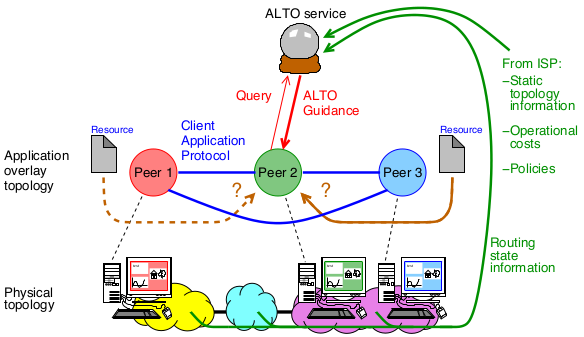
\includegraphics[scale=0.75]{alto-design.png}
    \caption{ALTO scenario \cite{seedorf2009}}
    \label{fig:alto-design}
    \end{figure}

    Despite its origins lying in the efforts to localize traffic in \gls{p2p} applications, the \gls{alto} protocol and its encompassing system is now being considered in other fields, to be now further discussed.

    A first area of interest is \glspl{cdn}, most specifically the on-going works in extending the base protocol to implement the \gls{cdni} Request Routing Footprint \& Capabilities Advertisement interface \cite{alto-cdni}, which is a subset of the \gls{cdni} standard \cite{cdni-problem-statement} that aims to allow upstream \glspl{cdn} to query known downstream \gnspl{cdn} for their willingness to accept content requests on their behalf.
    In particular, one of the main functionalities of the \gls{cdni} request routing interface is the ability for upstream \glspl{cdn} to retrieve static or dynamic information on download \glspl{cdn} (resources, footprint, load), which they provide themselves, and that allow the upstream \glspl{cdn} to better choose the appropriate edge server that could serve a given end-user.
    \gls{alto} serves as a good protocol to implement such functionality because it fits its use-case: some node wishes to improve its routing decisions to better decide on which other node to select, by using information that is hard, or nearly impossible, to independently retrieve. 
    Regarding \glspl{cdn}, the querying node is an upstream \gls{cdn} server that wishes to resolve their content requests by attributing the client to the most optimal downstream \gls{cdn} servers, where the content resides.
    At a more abstract level, this is similar to the use case discussed above where \gls{p2p} required assistance to more optimally select peer connections.

    Edge computing, similarly to \glspl{cdn}, uses a paradigm of flexible service distribution that enables deployment closer to the end user for better performance, and thus is inherently effected by network status.
    Current work is being made on how \gls{alto} can be leveraged to aid the task of deployment of functions or applications in the network edge \cite{alto-determining-service-edge}.
    Much like the previous example, \gls{alto} is being used to guide an application in a decision with impacts on both layers - by querying the \gls{alto} server, the client can retrieve information that regards to \gls{pop} where functions/applications can be deployed, such as cloud computing provider's available resources, e.g., \gls{cpu}, \gls{ram}, or storage, but also network information that pertains to the outside of the \gls{pop}, mainly network connectivity metrics, e.g., end-to-end bandwidth and delay, and routing costs.
    The utilization of the \gls{alto} protocol in this context would allow edge service clients and providers, as well as \glspl{isp}, the ability to combine efforts as a means to optimize edge computing deployment that considers the current network status, and doing so would thus result in benefits for both end-users and infrastructure maintainers.

        More broadly, current work is also being done in specifying abstract network entities path arrays between points \cite{alto-path-vector} and time-sensitive cost values \cite{alto-calendar-cost-map}, both of which share higher insight of the network, at the discretion of the \gls{isp}, as a means to provide even more context to applications about the infrastructure, such as identifying potential path bottlenecks and high traffic time peaks, respectively, and thus improve the ability of applications to optimally generate application traffic on the network.

    A mode of operation where applications no longer operate in disregard of the network infrastructure they run on, but instead in deep consideration of it, could help significantly alleviate the issues emerging from the tension between the underlay and overlay, and is of mutual interest - improving application performance and reducing infrastructural costs.
    Enabling a communication channel can thus allow for many different co-operational use cases besides the aforementioned ones.
    For example, redirecting users to nearby data caches or warning them of server maintenance ahead of time.
    The existence of an all-encompassing oracle could also prove beneficial for applications which utilize periodic network probing to guide their choices, as such information could be measured by a select few nodes in the network and applicable to all nodes which are close-by to such node in ways that the \gls{isp} deems advantageous, such as belonging to the same \gls{as} or geographically close by, thus minimizing the amount of otherwise redundant probing required by all application entities that wanted some network status information.
    \gls{isp}-guided counseling, however, does more than centralize measurements that could be done by the application itself.
    Besides containing measurements that could only be retrieved by the \gls{isp} itself due to its privileged access to the network, such as \gls{igp} packet inspections or secure \gls{snmp} queries, by handing over the decision-making process to the service provider entity, it is given power to better steer traffic in a way that favors internal policies and strategies, such as peering agreements, current traffic flow of other applications, known bottlenecks, etc., that could not be deduced by the applications alone.
    Thus, in the decision of how to generate application traffic, the responsibility should reside in both the application and the infrastructure as a way to benefit all relevant parties, i.e., the end users, the application stakeholders, and the service providers.
    \gls{alto} protocol serves an enabler of a mutually cooperative layer interaction system that, by becoming the standard, would aid towards a sustainable life-cycle of the Internet.

    Finally, standardizing an architecture and related protocols for a clear problem domain could help a large subset of similar issues, since a well defined and tested specification would exist, thus allowing many applications to leverage the \gls{alto} protocol's functionalities to their needs, not requiring further cycles of development for a specification when one already exists.
    Also, the attempt to standardize the oracle pattern is helpful as it joins forces from many different domains which share common problems - many of which were exemplified previously - into a single specification.
    A widely accepted and used solution can evolve from a combined effort, and would target issues such as security and scalability, creating a single point of convergence that is mature enough to be adopted with confidence, accelerating the transformation of the Internet as individual players would not need to develop their own specifications.

\subsection{Architecture}

    The high-level conceptual \gls{alto} architecture can be seen in Figure \ref{fig:alto-architecture}.
        Central to the operation is the \gls{alto} server, which stores network information and provides it to querying clients.
        Such network information is provided by trustworthy and relevant entities, as could be derived by routing protocols, \gls{isp}-specific policies, historic measurements, and feedback provided by third parties regarding application performance on the network.
        Two protocols can be seen as part of the general architecture: the provisioning protocol, which is not currently contemplated by the \gls{alto} working group, should specify how information is provided to the \gls{alto} server; the \gls{alto} protocol, which is the main focus of the working group with the same name, specifies server-client interactions as a request-response interface for retrieval of network attributes.
        The \gls{alto} client is the main consumer of the \gls{alto} service, and it queries the \gls{alto} server on network information whenever it deems such data as necessary to what it's doing at a given moment, with some potential use cases discussed previously.
        An \gls{alto} client could be seen as any entity which is able to interface with the \gls{alto} protocol with the role of a client, and as such is not tied to a specific implementation - in the example of \gls{p2p} file sharing, a peer can act as an \gls{alto} client (like the example scenario in Figure \ref{fig:alto-design}), but a tracker could instead take that role, enhancing its ability of assisting peer communication by having an embedded \gls{alto} client that would then act on behalf of peers when querying for \gls{isp} insight as to provide an optimal peer pairing.
        Using the tracker-oriented \gls{alto} client approach would minimize needed \gls{p2p} client protocol modifications and thus facilitate integration with currently existing applications.

    \begin{figure}[H]
    \centering
    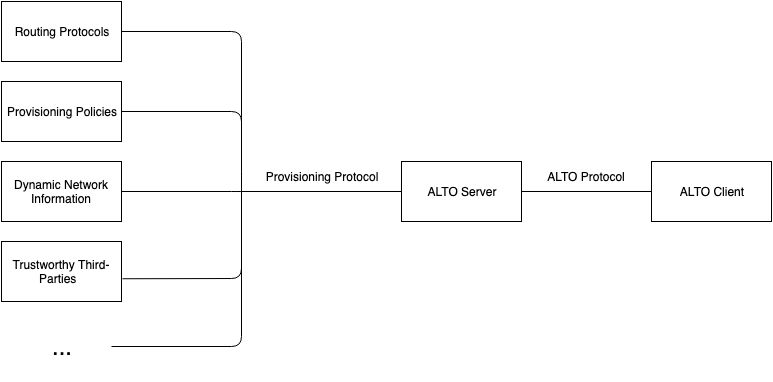
\includegraphics[scale=0.60]{alto-architecture.jpeg}
    \caption{ALTO architecture (adapted from \cite{alto-protocol})}
    \label{fig:alto-architecture}
    \end{figure}

    The \gls{alto} services contemplated by the working group can by visualized in Figure \ref{fig:alto-services}.

    \begin{figure}[H]
    \centering
    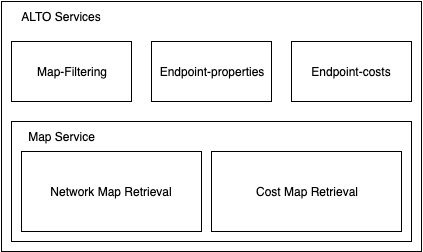
\includegraphics[scale=0.55]{alto-services.jpeg}
    \caption{ALTO services (adapted from \cite{alto-protocol}) }
    \label{fig:alto-services}
    \end{figure}

    The \gls{alto} server stores and provides special mappings in the form of network and cost maps.

    A network map provides network location grouping identifiers and the corresponding aggregated endpoints.
    It utilizes \glspl{pid} as a key, and the mapping itself is left to the responsibility of the providers - it is a way of indicating that many endpoints should be handled similarly.
    A provider can then aggregate endpoints by geographical proximity, one or many subnets, one or many \glspl{as}, etc., and attribute properties to the aggregate, instead of the endpoint.
    This is advantageous not only for scalability reasons - since it can compress information - but also because it allows \glspl{isp} to abstract network endpoints into groups, thus ensuring privacy of network topology details whilst maintaining useful network guidance, as the \gls{isp} has full control of how endpoints are aggregated, and consequentially how traffic is engineered since this changes how clients interpret resources.

    A second resource type provided is a cost map, which can be defined as a matrix M, where $M_{ij}$ - with i and j being the source and destination \glspl{pid}, respectively - is the associated path cost between the two indexes.
    The cost has two components: its metric and mode.
    The \gls{alto} base protocol only defines a single, generic, cost metric called "routingcost".
    However, \cite{alto-cost-metrics} is currently specifying more concrete metrics, with many associated with \gls{qos} evaluation, e.g., one way and round trip delay, packet loss and throughput.
    The other cost property, cost mode, can either specify that the metric is to be interpreted as a numerical value or as an ordinal ranking among all other costs in that cost map - this is useful in cases where too much network information is not deemed reasonable to share, and a simple order of preference that doesn't expose excessive infrastructural details can suffice.
    The decision to separate network and cost map information into two types of resources comes from the reasoning that network mappings are unlikely to change, whereas cost mappings could be periodically updated.
    As such, it alleviates client applications from the need to retrieve redundant information, and the ability to only retrieve a subset of it - this ability is further expanded in the map filtering service, which allows an \gls{alto} client to further specify which regions of the requesting maps it wishes to retrieve (much like a "SELECT" statement from an \gls{sql} database), and only these are transmitted.

    Finally, the last two services focus on mappings that regard to specific endpoints, instead of abstract mappings that utilize \glspl{pid}.
    An endpoint is currently identified by one of the following: \gls{ip} address, \gls{mac} address, or generic overlay ID.
    The endpoint property service maps to an endpoint a set of properties, e.g., geographical location or connectivity type, and the endpoint cost map has the same meaning of a cost map, but mapping to particular endpoints addresses and not abstract collections.
    The \gls{isp} has thus the ability to work with abstract aggregates or specific endpoints, showing as little or as much network information as it deems fit.

    As could be seen, the \gls{alto} project specifies an architecture for sharing of network-related information, with well defined roles and a request-response protocol to fulfill interactions between them.
    It also attempts to standardize such interactions in the form of data structures with well defined attributes which are then to be manipulated for each use case.
    This could then serve as a useful service for any application that wishes to retrieve network information as a means to improve its decision making at the application level.
    It is important to note that there are restrictions to what kinds of information are contemplated by the \gls{alto} protocol - for example, transport-level congestion is beyond its scope, and thus should not replace conventional mechanisms.
    The type of data which is valid to consider, according to \cite{alto-problem-statement}, should not be easily obtainable by the clients themselves - such as immediate end-to-end delay - and should be variable on a longer timescale than the instantaneous kinds that are seen on, for example, congestion control mechanisms, as the frequently resulting querying traffic would be counterproductive to the task of traffic optimization.
    Potentially valuable information that is in the \gls{alto} scope would then have to be harder to obtain without aid of this service, and not highly mutable through time - for example, routing costs, geographical locations, network proximity, operator's policies, scheduled down-times, historical application feedback, etc.

    This project is, at time of writing, still on-working, with many drafts being created and updated as the \gls{alto} project matures and increases its domain applicability.
    These are, however, relating to service extension and deployment, since the main architecture, protocol design, implementation guidelines and security analysis are fully published into their respective \gls{rfc} documents, serving as pillars for this work, and the ongoing efforts will serve as inspirations for potential extensibility.

\subsection{Viability}

\subsubsection{Security}
\label{ssec:alto-security}

    Given the nature of this system, particularly the trading of sensitive network structure information that can alter application behavior, it is quite apparent that its design and implementation are not without challenges from a security perspective.
    Indeed, the working group published discussions regarding security preoccupations at the development and deployment stages of the \gls{alto} system \cite{alto-problem-statement} \cite{alto-protocol} \cite{alto-deployment-considerations}.

    Utilizing the "STRIDE" threat model \cite{stride}, the main threats to the \gls{alto} architecture can be summarized as follows:

\begin{itemize}
    \item Spoofing of a legitimate \gls{alto} server that would mislead clients with wrong information - this could give the malicious party the ability to change traffic to its will.
        Spoofing of the clients themselves can also occur, and could allow a malicious party to retrieve sensitive network data outside their permission.
        Finally, spoofing of a provider of network status that could feed information into the server to be spread to applications, possibly misleading them in the same way an \gls{alto} server spoofing could, but by proxy.
    \item Tampering of data to mislead either \gls{alto} servers or clients.
        If some unauthorized and malicious party can retrieve data that is in transit or storage and tamper with it, clients would act on information that they assume is trustworthy but in fact has been modified.
        As such, clients could be redirected to wrong addresses, or receive incomplete or incorrect data that results in bad decision making.
        On the other hand, data tampering that occurs between data providers and the \gls{alto} server would give the latter, from a seemingly trustworthy party, untrustworthy data.
        This would result in the same issues that could arrive from spoofing threats.
        Tampering could also occur in input forms in the server-client or server-provider interface with potential to inject malicious code execution.
    \item Repudiation of being the source of some network information, whether it be by a third party that volunteered the data or the \gls{alto} server itself, which would make it difficult to neutralize and attribute culpability to incorrect or malicious sources, jeopardizing the legitimacy of the provided network information.
    \item Information disclosure in the form of \gls{alto} resources being made available to entities that were not contemplated to access it.
            These resources could give malicious parties insight on network topology status as well as the ability to derive clients' network usage patterns by observing what kinds of resources they attempted to retrieve at a given moment.
    \item \gls{dos} of the \gls{alto} server through request flooding beyond its capability, which would severely hinder - or even negate - its ability to serve legitimate users.
        By proxy, service denial of external entities can also happen through the manipulation of \gls{alto} resources themselves - leveraging the system's potential to guide traffic, if a given resource is manipulated in such a way that unreasonably favors the preference of a specific subset of servers, these could be selected by clients in a disproportionate matter, and highly affect these servers' availability.
    \item Elevation of privileges that lead to obtaining or modifying more information than initially permitted, resulting in the previous threats being heightened.
\end{itemize}

    Many of these threats are standard preoccupations for most computing systems and could be solved with state of the art solutions which are well proven and tested, as indeed states \cite{alto-protocol}.
    However, regarding threats of information disclosure - whilst they can be negated with in-transit encryption, what is done with this information the moment it reaches the client is hard to control - situations may arise when a client with proper resource permissions shares, intentionally or not, sensitive network information with other users who may or may not have proper clearance, in interactions outside the \gls{alto} architecture.
    Furthermore, many authenticated clients with different permissions could share information among themselves which they retrieved legitimately, to get a illegitimate complete view of the network structure.
    Thus, individual clients could internally collaborate outside the system to bypass access control measures applied inside it.
    As such, it is firstly important for the \gls{isp} or third parties to carefully plan on what information they are comfortable with sharing, knowing that it may be susceptible to future disclosure outside the secure domain.
    Possible solutions to minimize these threats include:

\begin{itemize}
    \item Reduce the granularity of the provided data.
        Intuitively, the less granular and precise the shared information by the \gls{alto} server is, the less valuable the resulting application guidance will be, and thus a balance would have to be found between layer cooperation and \gls{isp} privacy.
        One example is the usage of network groupings by \glspl{pid} instead of mapping information to concrete endpoints, working with network status around abstract entities.
        Another possible mean to reduce information granularity would be to utilize ordinal cost values, which instead of specifying a concrete metric, e.g., bandwidth in bits per second or packet loss in percentage, the server would give a relative preference rating with lower costs meaning lower preference.
        In both examples, the granularity of network information transmitted to the client is several levels higher in abstraction than the actual physical layer, and this could reduce the flexibility of applications to optimize traffic.
        However, they can still provide acceptable flexibility without impacting \gls{isp} privacy, acting as a much needed compromise.

    \item Work only with a small set of trustworthy \gls{alto} clients that are to act on behalf of a larger subset of less trustworthy clients.
        For example, network status resources could only be provided to authorized cooperation-oriented trackers in the BitTorrent protocol, which would in turn use this information to provide customized replies to clients without the need to change the base protocol.
        Similarly, information relevant for user-server assignment could only be provided to authenticated \gls{cdn} control nodes, who'd use among themselves a private virtual domain to share information about user-server connectivity and server status that would otherwise be inappropriate for any other type of user to retrieve.
        This is still, however, worthy of further threat analysis as restricted information could still leak outside of the system - beyond the means of spoofing discussed previously, seeing how a system behaves with \gls{alto} guidance can give - albeit limited - insight into SP bias.
        To see this, consider how a BitTorrent peer could continuously query a tracker with carefully crafted parameters - such as source address and candidate peers - and attempt to derive information from the resulting action, or similarly how a end-user could utilize similar parameter modification to observe the edge server selection mechanism in action.

    \item Utilize terms of agreements that are to be enforced on every querying client, stating that network status information does not get used beyond its original purpose, prohibiting sharing.
        Although a potentially helpful mechanism to dissuade malicious users, it can be deemed impractical to apply, especially considering the scale at which this information could be shared.
        Thus, utilizing such means should be applied at a case-by-case situation and it should not replace \gls{isp} discretion and server resource maintenance to ensure a given standard.
\end{itemize}

\subsubsection{Privacy}%

    Privacy concerns are also very prevalent in the \gls{alto} system, being an ubiquitous talking point in most of the working group's problem statements and protocol specifications.
    When an \gls{alto} client queries a server for one or more network status resources in the attempt to optimize the application traffic it will generate in the near future, certain parameters can be passed to the server that can make the response be more personalized and contain more granular information.
    For example, a real-time \gls{p2p} media-streaming application seeking \gls{alto} guidance to help choose among a list of candidate streaming peers may wish to include in its query helpful parameters such as the peer list itself, the desired \gls{qos}, and the network position of the querying client itself.
    Indeed, these and more patterns will help increase the effectiveness of the \gls{alto} server's guidance in helping the client application achieve its goal, but such happens at the expense of potentially allowing an \gls{alto} server to infer on user pattern statistics.
    Even assuming that the previously discussed information disclosure threats are nonexistent in the \gls{alto} system, privacy concerns can arrive from client applications because the resource queries they need to produce can contain information about what the client either will or wants to do.
    This is recognized by the \gls{alto} working group as a possible concern \cite{alto-protocol} \cite{alto-problem-statement}.
    In response, they state that the clients should firstly be cognizant about the potential tracking risk that is associated with the usage of the system and, as an attempt to make tracking harder, they could disable \gls{http} cookies and/or opt for more vague query parameters, e.g. by randomizing some bits on endpoint addresses or simply using more broad addresses, whilst being aware that the helpfulness of query results may vary with increased parameter obfuscation.

    Very much like client privacy, \gls{isp}-related privacy is also considered by the working group.
    \glspl{pid} were created as a means for \glspl{isp} to abstract network components as a collection of single network endpoints with similar properties, helping them not to disseminate network information that is too sensitive, and in turn also allows clients to make queries based on these identifiers and maintain a higher level of privacy.
    An ongoing proposal for protocol extension includes path vectors \cite{alto-path-vector}, that aim to represent information on the intermediary hops from a given source-destination pair, and each of these hops is represented as an \gls{ane} that, similar to \glspl{pid}, give \glspl{isp} the ability to under or over-abstract the topological representation that gets published to clients, giving more options to balance guidance usefulness with provider privacy.
    Other solutions could also be considered depending on the needs of the clients and the direction of the project as a whole.
    For example, the servers themselves could operate on a secure communications channel and maintain a clear agreement on what can and cannot be made with the collected information.
    Alternatively, clients that wish not to impose much trust on the server's claims not to track them could make bulk queries (or use proxies to do so for them) and privately filter out the relevant information, heavily restricting on the ability to retrieve user activity patterns.

\subsubsection{Incentivisation}

    Incentivization relates to creating and divulging, to both layers, incentives to a fully cooperative layer relationship that is inherent in the oracle pattern adopted by the \gls{alto} system.
    It is quite the challenge to fundamentally change how applications behave on the Internet, as indeed is to ask of \glspl{isp} to launch a view of their infrastructure to the outside world.
    \cite{dan-Commag10} notes incentivisation as one of the key challenges in overlay-underlay cooperation in regards to \gls{p2p} applications, stating that incentive mechanisms need to exist to ensure that both layers agree to participate in, and maintain, a cooperative relationship.
    According to the \gls{alto} problem statement \cite{alto-problem-statement}, the incentives for both parties to act on the system are the advantages that derive from using it.
    Meaning, clients are to expect better application performance by leveraging \gls{alto} guidance, and similarly \glspl{isp} should expect that their internal goals, such as an optimization of infrastructure utilization, can be met with the increased traffic engineering ability that results from their oracle role.
    If the overlay consuming \gls{alto} guidance has a manageable number of accountable entities, such as a single \gls{cdn} or data center that the \gls{isp} agrees to partner with, it is realistic to maintain a cooperative agreement that can be solidified with feedback and service agreements.
    However, if the overlay utilizing the \gls{alto} system makes it hard to pinpoint accountability, such as a large \gls{p2p} application with many users, it will naturally be harder to ensure that the power dynamic between layers doesn't shift beyond an equilibrium.
    In these cases, policies could be created and enforced to give insurance to both parties that a cooperative relationship is maintained.

    The \glspl{isp} could too, like mentioned above, lack proper cooperation, as they are found in a new power dynamic that would leverage their application traffic engineering capabilities to steer traffic in a way that is advantageous to only them, or at least in a disproportionate manner.
    Again, much like the lack of cooperation by clients, it is difficult to guarantee an equilibrium in the power dynamic between layers, but by guaranteeing improved \gls{qos} levels for applications that utilize \gls{alto} cooperation, \glspl{isp} become responsible for guaranteeing that these improvements are met, fearing client abandonment otherwise.
    Giving freedom to both layers on how they act ensures that the system evolves to a common ground that benefits both sides, at least enough to justify them remaining there.

    Finally, if the application-\gls{isp} tussle becomes harsher and unmaintainable, which is a point that was argued for in the network infrastructure effects portion in Section \ref{sec:state-of-art}, a cooperative system such as \gls{alto} may become necessary, and thus beyond preferable, meaning that \glspl{isp} may be forced to block or throttle traffic that it cannot route properly, as it historically happened.
    Thus, acting with \gls{alto} could go beyond a voluntary action into a symbiotic necessity, meaning that both parties have to act cooperatively to maintain network sustainability.
    Regardless, the best approach seems to be that the system must in of itself be self-justifiable, meaning that the advantages that it brings should be enough to convince both parties to act on it.
    \glspl{isp} are nevertheless free to deploy their own incentive mechanisms to facilitate early application adoption, that could include monetary rewards or routing privileges, but doing so could damage network neutrality.

\subsubsection{Network Neutrality}
    As stated by \cite{qos-framework}: "According to most network neutrality proponents, network neutrality rules are intended to preserve the Internet's ability to serve as an open, general-purpose infrastructure that provides value to society over time in various economic and non-economic ways. In particular, network neutrality rules aim to foster innovation in applications, protect users' ability to choose how they want to use the network, without interference from network providers, and preserve the Internet's ability to improve democratic discourse, facilitate political organization and action and to provide a decentralized environment for social, cultural and political interaction in which anyone can participate.".
    Network neutrality has been a popular point of discussion as society grows around the Internet, sparking debates around the world on what the best course of action should be - for example, regulations were introduced by the \gls{fcc} \cite{fcc} in the United States to police network neutrality \cite{fcc}, and the European Union has a framework for net neutrality laid down in Article 3 \cite{article-3}.
    However, potential violators of the spirit of a network neutrality exist, such as British Plusnet's \cite{plusnet} usage of \gls{dpi} to implement limits and differential charges for different traffic \cite{arstechnica}, or Portuguese MEO's \cite{meo} smartphone contracts which include zero rating programs for a given set of services \cite{meo-packages} that bundle applications such as Facebook \cite{Facebook} or Spotify \cite{spotify}.

    Network neutrality advocates are concerned with guaranteeing that \glspl{isp} keep Internet communications free and do not discriminate based on the traffic's specifics, such as platforms, applications, or source and destination addresses.
    On the other hand, opponents of net neutrality, among them the \glspl{isp} themselves, broadband and telecom companies, and hardware manufactures, argue against net neutrality - they claim that it would would reduce incentive to invest, as investments would be harder to insure without the ability to charge higher rates for better infrastructure capabilities.
    Zero rating programs, such as Wikipedia Zero \cite{wikipedia-zero}, which provide Wikipedia \cite{wikipedia} pages with no charge to a select group of low income regions, are popular in developing countries \cite{network-neutrality-developing} , provide to select regions Internet content they could not otherwise get, but in the form of a non-neutral view to the network.
    Additionally, with net neutrality, the \gls{isp}'s ability to route traffic could itself be at jeopardy - as \cite{qos-aware} states when he argues for a solution that compromises net neutrality via service differentiation, the Internet is growing at an astonishing rate, as are the demands of applications, and operating the infrastructure on a purely best-effort basis will not be sufficient without a constant provisioning of such infrastructure to keep up with demand, and this too may not be economically viable nor even possible.
    Thus, discriminating by traffic services may be needed to guarantee that, say, real-time medical information gets priority over real-time media streaming, which in turn gets priority over e-mail or file sharing.

    Considering that the \gls{alto} system behaves in an oracle pattern of cooperation where a single entity - the \gls{isp} - is able to heavily influence the traffic patterns of the applications it aids, on the promise of a cooperative network underlay-overlay relationship, such system could violate the principles of net neutrality.
    In particular, this could happen if the oracle either blocks, or at the very least provides different guidance to different clients, depending on where the query originated from - e.g., which application, which source address, or other defining characteristics.
    A possible consequence of such a system guiding the Internet could be that given applications can consistently have better \gls{qos} measurements not on the basis of the application's implementation, but on the \gls{isp} personal biases.
    Oracle systems such as \gls{alto} do not seem to be analogous to other traffic engineering strategies, such as the usage of \gls{mpls}, \gls{diffserv}, nor to other means of \gls{isp} intervention on overlays, such as the deployment of data caches and redirector proxies - this is because the oracle system, in contrast to the previously mentioned strategies, is one of mutual voluntary and cooperative nature between \glspl{isp} and applications.
    However, it could be argued that if the \gls{alto} system offered guidance to applications in such a way that consistently resulted in better application performance, such applications would be pressured to use such guidance as a means to remain competitively viable, and the \glspl{isp} would then have a platform to influence a considerable amount of traffic to their will, being in a position to, depending on how they treat guidance requests, break network neutrality.
    This neutrality concern can be alleviated if application guidance operated on classes of traffic, e.g. real-time communication or file sharing, thus operating on traffic aggregates to insure \gls{qos} levels needed to given application types, but never discriminating beyond such given classes.

    As the protocol is defined \cite{alto-protocol}, the provided network status information is truthful and guidance is optional, and neutrality can then still remain outside of the system, since no routing measurements exist within it.
    If particular implementations of the \gls{alto} system give guidance in such a way to guide traffic in a discriminatory fashion, and if such guidance has advantages that much outweigh any alternative, thus rendering it beyond optional,  a case can be made for how \gls{alto} as a concept can break network neutrality, considering all its advantages and disadvantages discussed below, as the \gls{isp} can utilize discriminatory behaviour to treat applications on their infrastructure differently.

\subsubsection{Multi-Domain orchestration}

    The Internet as we know it today spans the entire globe and is rather complex in nature.
    According to \cite{dan-Commag10}, the classic vision of the Internet consisting of a network of transit and stub \glspl{as} no longer seems accurate, as it now is much more complex - for starters, the role of network owner and service provider are separating, and Internet access is provided by numerous competing \glspl{isp}.
    As a demonstration of such complexity, Figure \ref{fig:network-connectivity-globe} displays how the Internet is structured into many tiers of different service providers.

    Considering this administrative complexity in the Internet's topology, it can thus be inferred that the act of layer cooperation can get harder when the influence domain increases and potentially spans many different \gls{isp} regions which will inevitably act differently as they can have different technologies, biases, policies, and overall goals.
    These per-\gls{isp} biases can make it difficult to guarantee that traffic optimization spanning multiple administrative domains is actually useful and achieves the cooperative nature in mind.
    For example, an \gls{isp} may not be comfortable categorising end-point costs of a given metric, thus making path calculations that pass through that \gls{isp} domain not viable.
    Regardless, per-domain \gls{isp} guidance has nonetheless plenty of potential, e.g., the ability to localize traffic, as entities outside of domain can be identified by \gls{isp}, and similarly per-domain optimization of resources can still be useful when such domain is large, and can be applied to high-volume operations such as those in a data center.
    The \gls{alto} server within a given domain can also leverage probing measurements and feedback statistics to derive information in areas whose topological detail is unknown, giving a partial network view that contains topological insight and also information derivation that, whilst not being as good as a complete topological insight, may nonetheless power a cooperative effort within a given domain with good results.
    Some data may, whoever, be both not shared by an external domain nor derivable.
    This includes endpoint property information, such as network connection types, or server footprints, e.g., available \gls{cpu}, \gls{ram} and storage.
    This information can in some conditions only be retrieved by authoritative entities in a given domain and probing solutions may not be available, thus considerably limiting the applicability of a single \gls{alto} domain.

    \begin{figure}[H]
    \centering
    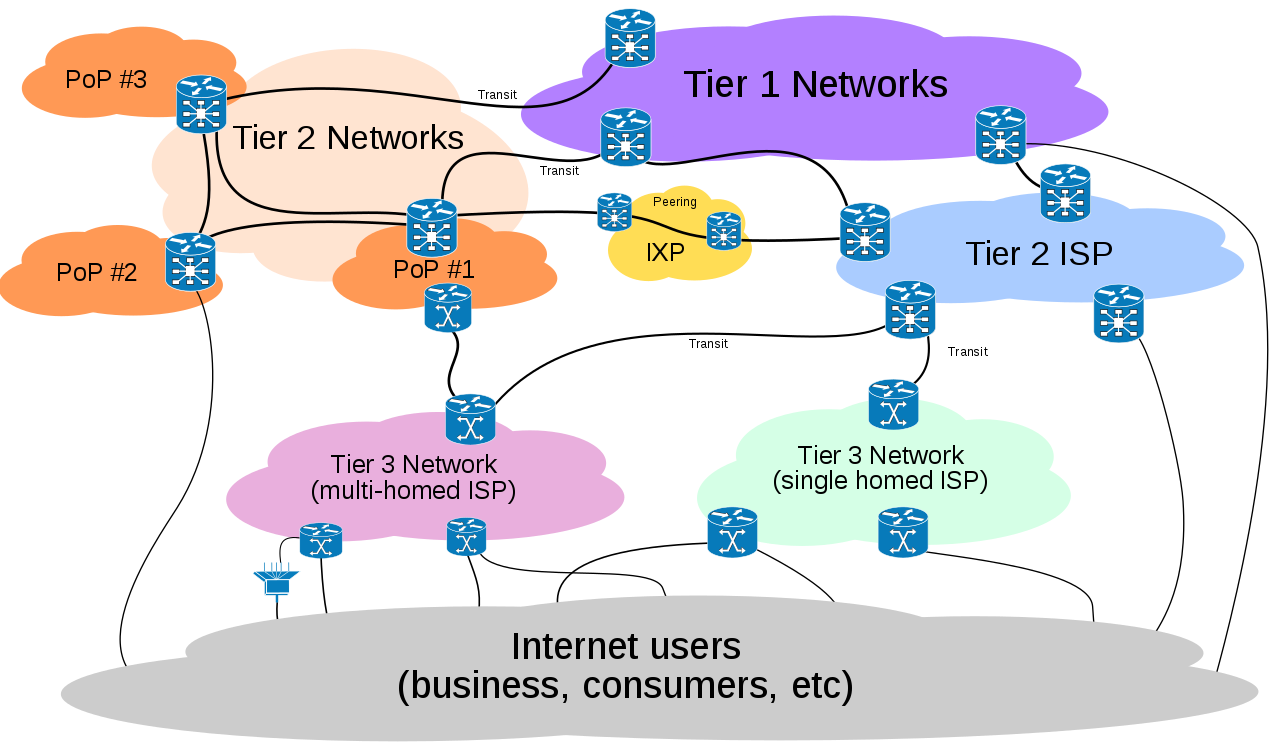
\includegraphics[scale=0.30]{network-connectivity-globe.png}
    \caption{Conceptual representation of ISP diversity on the Internet}
    \label{fig:network-connectivity-globe}
    \end{figure}

    Even assuming that all \glspl{isp} are comfortable with sharing sufficient information, ambiguity may arise.
    For example, considering a cost map with the generic "routingcost" cost metric, \glspl{isp} could internally calculate routing costs differently, and prioritizing different goals, e.g., reducing overall link usage versus reducing inter-\gls{as} traffic first and foremost.
    The base \gls{alto} protocol specification states that each network region can provide its \gls{alto} services, which in turn convey network information from their perspective.
    A network region, per the protocol specification, consists of a given administrative domain, such as an \gls{as}, an \gls{isp}, or a given set of agreeing \glspl{isp} \cite{alto-protocol}, thus implying that if multiple \glspl{isp} share an \gls{alto} server they must reach a consensus on what network status is available for query from the outside.
    Furthermost, the \gls{alto} working group's deployment considerations \cite{alto-deployment-considerations} document states that an \gls{alto} client can query a single server for one or many metrics, or he can additionally query multiple server instances on different networks \cite{alto-deployment-considerations}.
    It is explicitly stated in the document that each server could give guidance for only a given network partition, and such guidance may wildly differ between them due to the fact that different algorithms and objectives may have been applied.
    The document also states that, in regards to extending the reachability of a single server, three different strategies could be applied:

\begin{itemize}
    \item \textbf{Authoritative Servers}: A given set of servers can provide guidance for all kinds of destinations to all \gls{alto} clients.
    \item \textbf{Cascaded Servers}: An \gls{alto} server can possess an embedded \gls{alto} client and query other neighbouring servers if it cannot serve the original request, acting as a middleman between the client and the more appropriate servers.
    \item \textbf{Inter-server Synchronization}: Different \gls{alto} servers communicate among themselves to expand the knowledge space.
\end{itemize}

    The last strategy is still being subject to development and standardization by the working group as part of a bigger attempt to link different network regions and technologies into a single, homogeneous abstraction of the Internet.
    Current efforts in multi domain orchestration and relevant use case examples are summarized in the ongoing work of \cite{alto-multi-domain-use-cases}.

\section{Summary}

    In the taken case studies seen in this chapter, it can be clearly seen that there is room for improvement in application-layer traffic generation that can benefit both the applications themselves and the infrastructure administrators that support them.
    Applications struggle to achieve optimal network resource utilization, whether that be in the task of matching peers in overlay networks, deploying and attributing edge server to media clients, selecting mirror servers, etc., and solutions are being continuously proposed and created that attempt to optimize these decisions.
    Traffic optimization solutions vary between them with the range of control that is given to the overlay and underlay parties.
    It seems to be the case that one-sided solutions can hurt the other layer in a worse case scenario, and be lacking maximum efficiency at the best.
    \gls{alto}'s proposal seems to bridge the best of both types of proposals that are either underlay or overlay-centric, standardizing a system and associated protocol whose purpose is to achieve layer cooperation so proper network utilization is possible.
    Despite many of its associated challenges - namely in the regions of security, privacy, and incentivisation - the project certainly has the potential for a more resourceful Internet that can be more sustainable.

\chapter{System Architecture and Developed Mechanisms}

    As the main proposed goal of this work is the implementation of a system that complies with the \gls{alto} working group's devised protocol, this chapter exhibits the planned software specifications needed to implement the system as a whole, with the aforementioned protocol being a crucial part of client-server resource exchange.

    Initial attention is given to the general architecture on the first section, with the goal of identifying key entities, their purpose, and how they interact among themselves.
    The following section will target the specification of \gls{alto} resources, which can be considered the driving force behind the system, as they are what the client entities seek, and likewise what the \glspl{isp} wish to provide.
    The next section will focus on specifying the task of network status provisioning to an appropriate \gls{alto} server, in such a way that a common interface exists among all entities that are able to increase the server's knowledge of the network's physical topology.
    Upon specified the way that network information is provided, the next section details how a given actor, such as an \gls{isp} administrator, can pre-process such information before it is forwarded to the server and available to clients.
    Finally, the task of multi-domain \gls{alto} server synchronization and communication is specified in the form of required protocol extensions and needed mechanisms that allows the increase of a single \gls{alto} server's knowledge space.

\section{General Architecture}

    Figure \ref{fig:architecture-network} presents a high-level conceptual model of how the network information flows in a given \gls{isp}.
    Network data originates in the topology itself, and is gathered into a network information aggregator by the appropriate means - this aggregator defines an interface through which network data can be uploaded, and entities utilize it to provide the network data they have collected.
    These entities will use different means to gather information, as the Internet is supported by a massive variety of protocols and standards for network and resource information querying.
    For example, a node could deploy a daemon listening for \gls{ospf} protocol packets to gather path cost information, and another using \gls{snmp} to gather node property information.
    Obviously, since the interface simply defines how raw data must be formated to be accepted by the network information aggregator, means through which the data is uploaded are left to the source itself, and because of this static data uploads that were previously collected could be used instead of dynamic retrievals - for example, the network administrator could use previously collected information that resides in a database and upload it as is.
    The network information aggregator serves as a hub for network administrators to process the raw network data that was collected by the previous tier, and transform it into \gls{alto} resources ready to be accepted and distributed by the corresponding server.
    This task of network information processing is where \gls{isp} policies and preferences are injected via, for example, the abstraction of network entities with the aggregation of network addresses into \glspl{pid}, and the creation of cost maps which result from the transformation of network link information mixed with given \gls{isp} goals.
    If, say, the administrator wished to provide a cost map between network entities which aimed to reduce inter-network traffic, it would firstly aggregate endpoints into abstract entities with common properties, as an attempt not to share too much infrastructural information, and then use the previously collected network link information, attribute higher costs to undesired links, and transform it utilizing the Dijkstra's algorithm to create a shortest path map that is bound to provider preferences.
    Such map is then parsed as an \gls{alto} resource - more specifically, a cost map - and afterwards uploaded into the \gls{alto} server with the access policies the administrator sees fit.

\begin{table}[H]
\centering
\caption{Network node entities in the conceptual ALTO system representation}
\begin{tabular}{ | c | l |}
\hline
\textbf{Image} & \textbf{Description} \\ \hline
\raisebox{-.30\height}{
\includegraphics[width=8mm]{img/circle-white}} & Network node \\ \hline
\raisebox{-.30\height}{
\includegraphics[width=8mm]{img/circle-blue}} & Network node participating in a given overlay network \\
\hline
\end{tabular}
\end{table}

\begin{figure}[H]
        \centering
        \hspace*{0.35cm}
        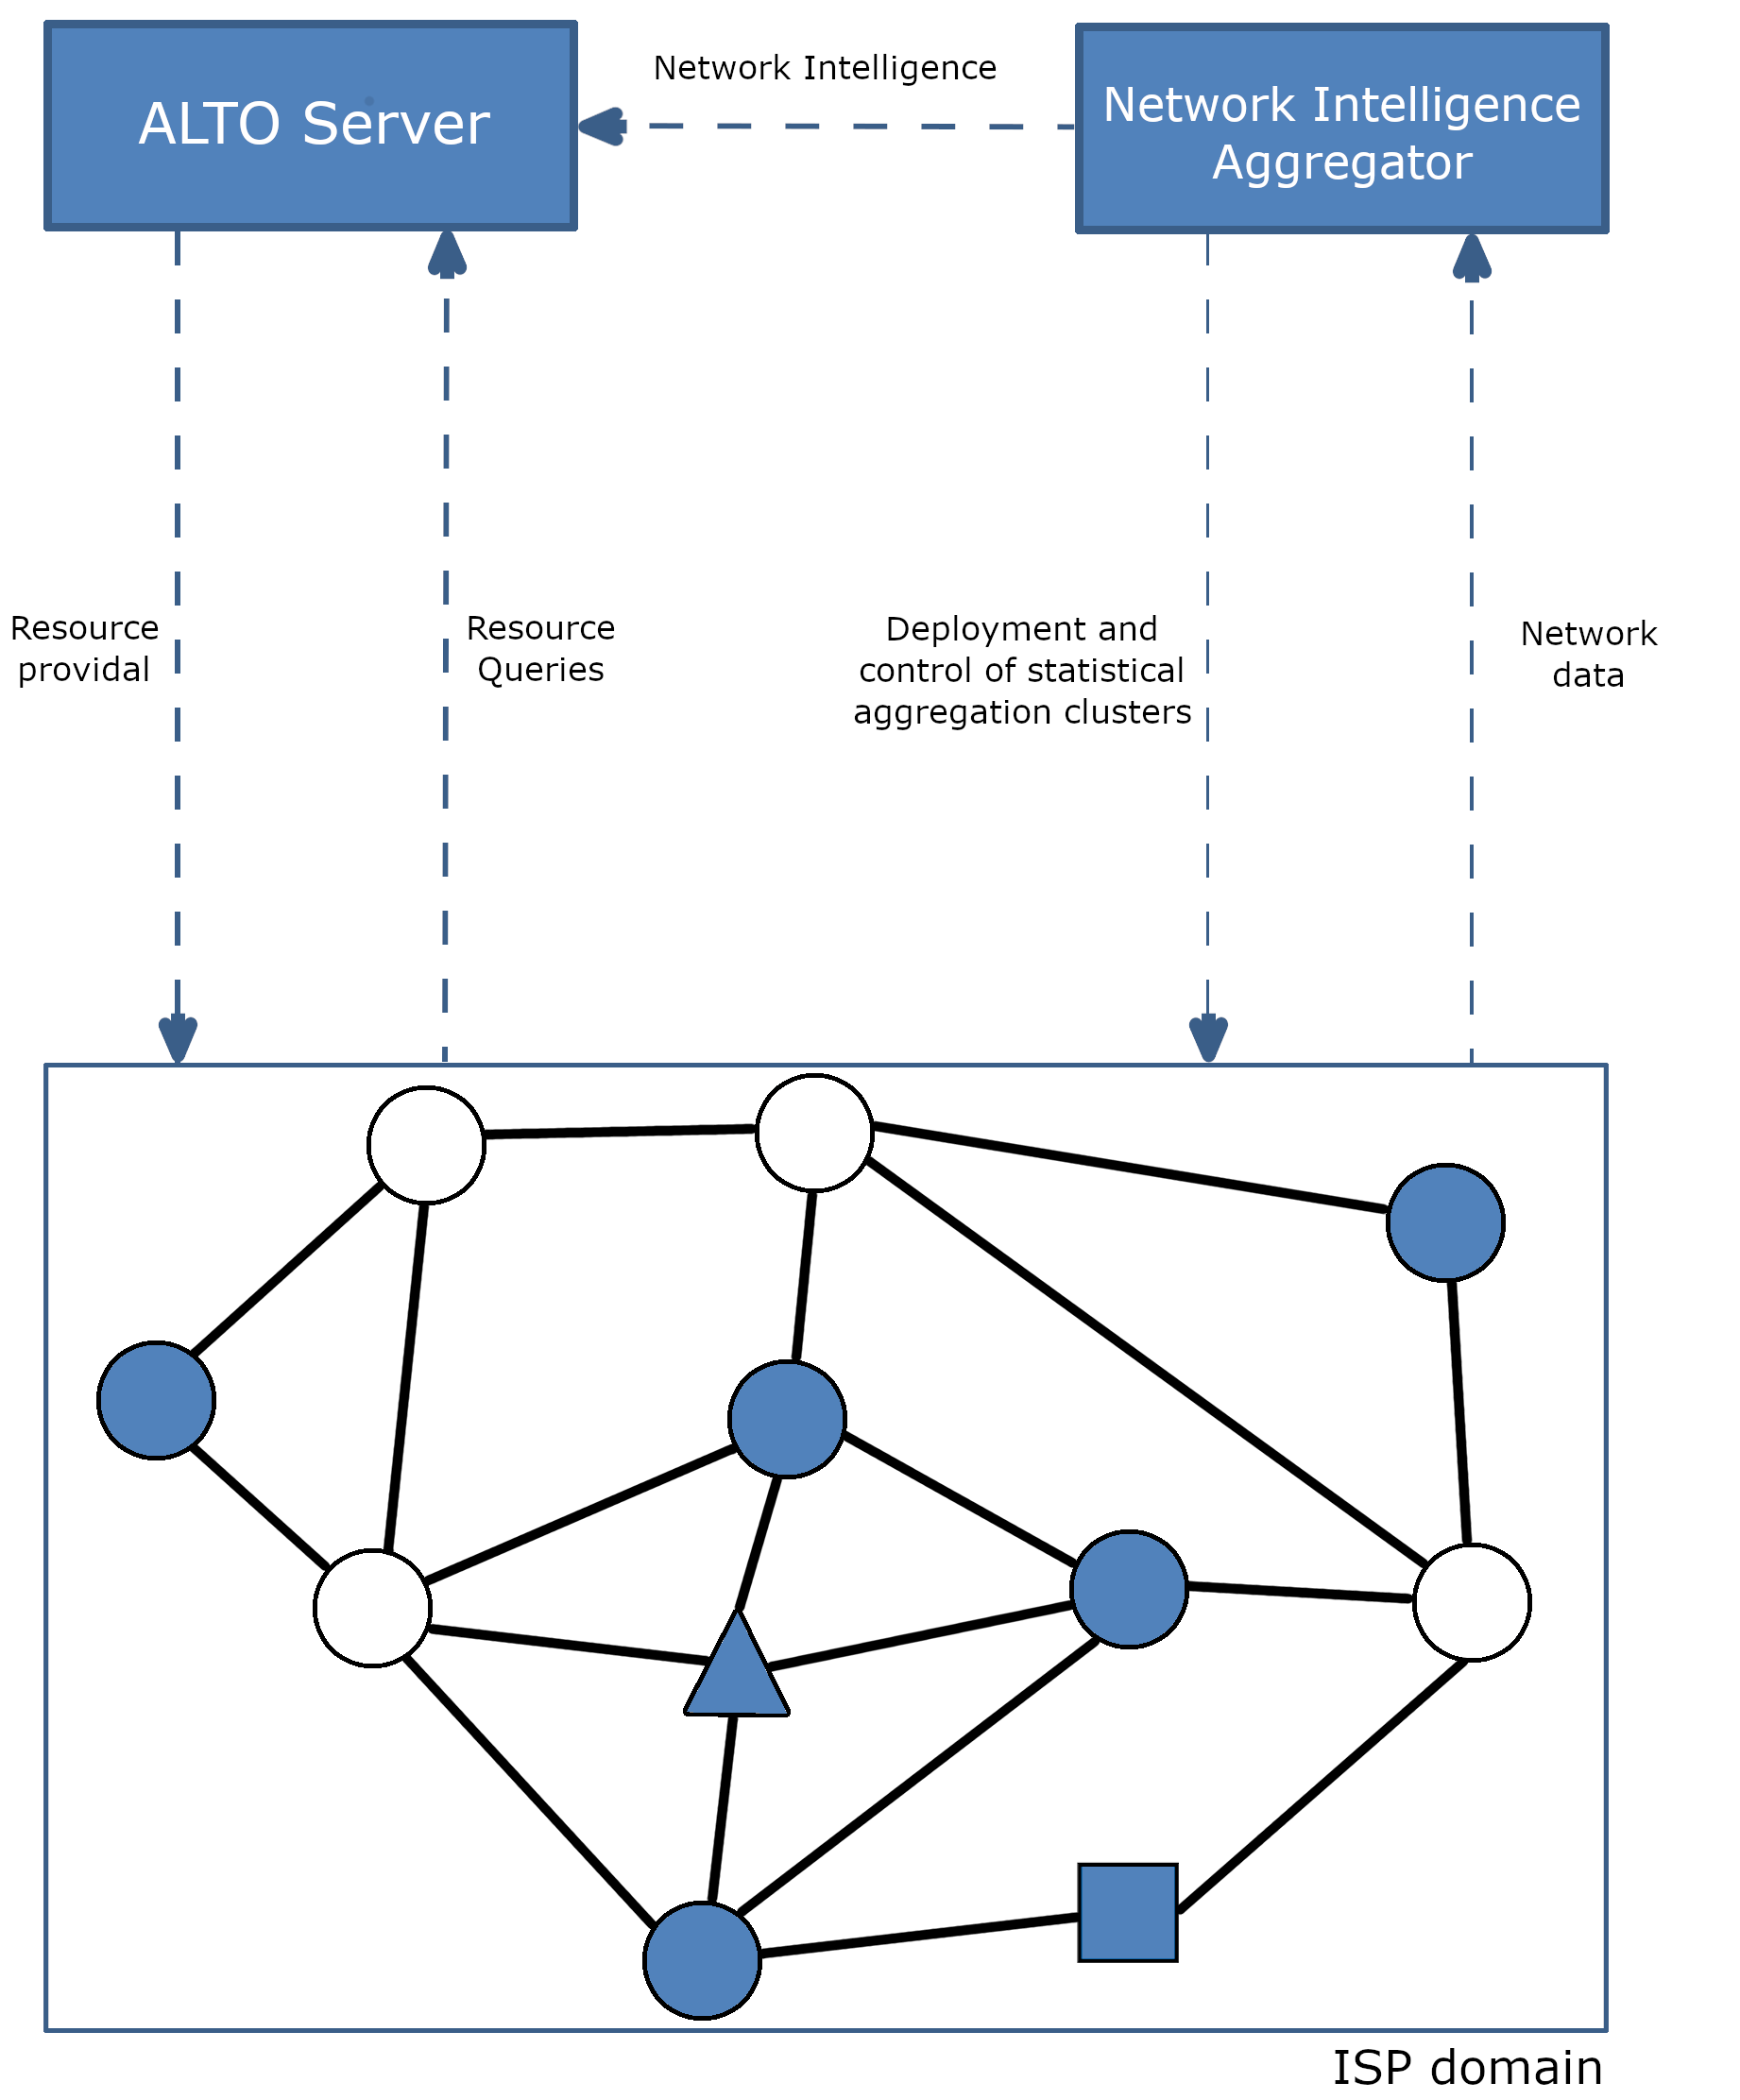
\includegraphics[scale=0.75]{img/architecture-network.png}
        \caption{Conceptual representation of the ALTO system of a given ISP}
        \label{fig:architecture-network}
\end{figure}

    More formally, Figure \ref{fig:macro-architecture} presents the proposed system architecture.
    One can identify the \gls{alto} interface - logically separated in its download and upload components - as a key factor of the system, as it allows to bridge three different application layers - the \gls{alto} resource consumer, the \gls{alto} resource provider, and the network information aggregator, to be further specified in the following sections.

    The \gls{alto} working group has extensively specified the \gls{alto} protocol, which regards to resource querying, and the concrete implementation of this work will aim to comply to it.
    However, no resource provisioning protocol was, at time of writing, specified by the working group, nor was an interface been specified to allow network data to reach the \gls{alto} server.
    It has been set as a work in progress, and the topic of network information sources was briefly discussed in \cite{alto-deployment-considerations}.
    The working group has grouped the tasks of raw network processing and supply into the role of the \gls{alto} server.
    However, as can be seen in the proposed architecture, a different approach was taken in this work, with the roles being separated and an additional protocol proposed to bridge communication between them.
    This was made as an attempt to adhere to the philosophy of single responsibility, making the sole task of the \gls{alto} server the management of \gls{alto} resources.
    This aims to facilitate the independent development of the different roles, and make it easier to interchange implementations - this would make it particularly useful, for example, to deploy many \gls{alto} servers in a cascade fashion whilst utilizing only a single network information aggregator.
    These are, however, only conceptually separated, and an implementation could, if it is more practical, merge the server and information provider roles into a single physical entity - which would then be similar to the architecture designed by the \gls{alto} working group.

    As most software architectures, each new communication channel represents a possible source of attack vectors and, attending to the critical security concerns posed in Section \ref{ssec:alto-security}, all of these channels must be secure and reliable, as signified by the padlocks on the presented architecture.
    This implies that data communications within it must be block being read or altered by non authorized users, and the identity of the participating parties can be trusted and made accountable.
    The identified communication channels must then have methods of maintaining data integrity in transit, user authentication and authorization, and communication confidentiality.

\begin{figure}[H]
        \centering
        \hspace*{-4em}
        \includegraphics[scale=0.25]{architecture-macro.png}
        \caption{System architecture at a macro level}
        \label{fig:macro-architecture}
\end{figure}

\section{Role system}
\label{sec:system-roles}

    As an access control measurement, the system will work with \gls{rbac} methods which, as the name states, center their control policy logic around roles, which themselves are tags that can be attributed to users.
    A pre-requisite is then that users attempting to access a system employing \gls{rbac} must be authenticated as a given user, and from then a list of attributed roles can be retrieved to validate if a given action is permitted according to the set rules.
    The \gls{alto} resources - the main interest of this system as it is the data component requested by clients and managed by the servers - has associated to it an \gls{acl}, that maps, for a given set of roles, the list of user actions that are allowed to be performed to that resource, with the implicit rule that a resource's owner has full clearance.
    The available user actions are "read", "update" and "delete", meaning the ability to get, change the contents of, or remove the resource, respectively.
    This \gls{acl} must be provided by the Network Information Aggregator whenever a new resource is inserted into the \gls{alto} server.
    The \gls{isp} administrator that controls the aggregator not only then designs the resource itself - adding the information that it deems important whilst not too detailed to damage privacy - but also defining access control policies on that resource, which will be then enforced by the server in future requests.

    Employing access control based on roles seems appropriate for this system since roles can be applied to - and thus group - many users, and indeed that seems to be applicable on real case deployments of the \gls{alto} system - each given application, that consists of a great number of users, can correspond to a single group, and more private scenarios, such as a data center server cluster, can also be grouped.
    This facilitates permission management, as the \gls{rbac} approach allows grouping of permissions into roles, which can then be quickly manipulated to affect every user associated to it - this would contrast to an approach where permissions are set per user, which would be considerably harder to manage at scale.
    As a user can be granted many roles, he can naturally act on the system with a role that fits the currently queried resource, if so applies, and likewise the network administrator can give permissions per role, which in turn can group as many as millions of users, or to just a single one.

    An \gls{rbac}-based access control mechanism will help mitigate security threats pertaining to the \gls{alto} working group's architecture - e.g. having unwanted users reading or tampering with data.
    However, for such mechanisms to be viable at all, authentication systems need to also be employed to help verify that the users are indeed who they are announcing to be.
    Authentication mechanisms are, regardless, of extreme importance, as they additionally help mitigate spoofing security threats.
    Data breaches are not, however, totally mitigated with authenticity and access control mechanisms.
    After an entity gets a resource and acts outside the system, it becomes out of its control and these mechanisms cannot be employed.
    This means that there are no guarantees that the resources are shared outside of the system's domain and consequentially there are no security guarantees after that point.
    Because of this, privilege attribution by the \gls{isp} administrators not only give clearance to do a certain action, but also imply that trust exists that these users will not be improper with the given resources, such as sharing it with users with improper clearance.

    Figure \ref{fig:communication-roles} provides a high-level communication diagram of how access control is enforced - the \gls{isp} administrator that uploads the resource into the \gls{alto} server appends to it an \gls{acl} that maps actions to the considered roles, with the implied meaning that those that weren't considered have no permitted actions.
    When a resource consumer requests an action - which is expected to be a "read" one - and proper authentication was performed to verify its identity, the server checks that the roles associated with that consumer have the requested action allowed in the \gls{acl} and, if indeed that is the case, the action performs as expected.

\begin{figure}[H]
        \centering
        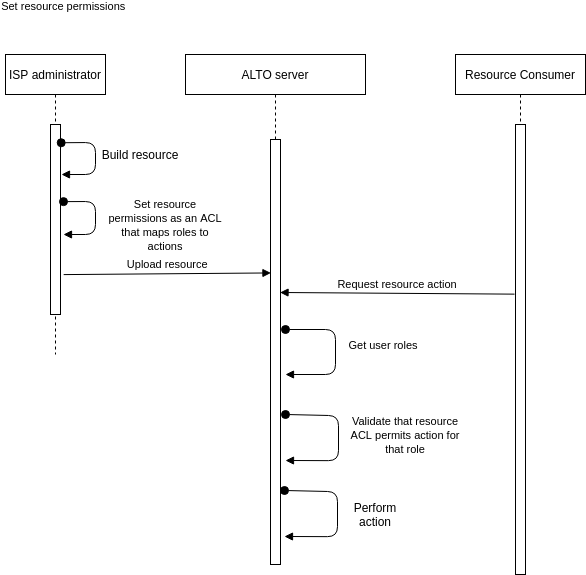
\includegraphics[scale=0.55]{communication-roles.png}
        \caption{High-level communication diagram of a successful resource action request}
        \label{fig:communication-roles}
\end{figure}

\section{Resources}
\label{sec:alto-resources}

    \gls{alto} resources are pieces of network information which are provided by an \gls{alto} server and consumed by \gls{alto} clients that ideally would use such information to aid their application-level traffic decisions.
    All \gls{alto} resources can be separated into the following components:

    \todo{talk about scope}

\begin{itemize}
        \item \textbf{Meta information}: Data which regards to the resource's profile, that enable the client's ability to interpret and cross-reference the network data within.
            Meta information contains the resource's name, and if applicable, version, resource dependencies and cost details: enclosed cost modes, metrics, and descriptions.
            Finally, also belonging to the meta section of the resource's information is the resource's \gls{acl} which, to a given set of roles, specifies the allowed set of actions.

        \item \textbf{Network status information}: Data structures that give a characterization of the \gls{alto} Server's vision of a network.
            Concretely, these can map network properties to a node - such as the connection types of their interfaces, or their geographical location - they can aggregate many network addresses to a single identifier, or they can map properties to a node link or end-to-end path - such as link or cumulative routing costs.
\end{itemize}

    Meta information can be seen as a resource's header, containing data that regards to the network status and helps better handle it.
    Following the defined protocol \cite{alto-protocol}, this field includes the resource's name for all resources, which is needed for identification and indexing, and all other fields are dependant on the type of resource: at this version of the protocol, only network maps are version-able, allowing \glspl{isp} to reference different versions of a network map as they are updated, maintaining support for previously referenced versions; cost information is, naturally, only applicable to cost maps, and gives insight on how the numeric costs are to be interpreted, i.e. what their mode and metrics are, and what description it has.
    Finally, extending to the protocol is the addition of an \gls{acl} as a solution to access control needs.
    An \gls{acl} is defined as a matrix, with each entry defining a user role and actions - discussed in Section \ref{sec:system-roles} - as a restriction on what a given user was given clearance to do.

    The network status information of a network map groups endpoint addresses into a single \gls{pid} as a text literal.
    Akin to the working group's protocol, accepted endpoint address protocols include \gls{ipv4} and \gls{ipv6}, utilizing a 32 bit long bitmask to identify a subnetwork.
    Similarly, support for aggregation of \gls{mac} addresses was added, with a 48 bit long bitmask to identify address ranges, similar to the \gls{ip} variant.
    Additionally, generic overlay IDs can be added with the key "priv:X" - with "priv" meaning private scheme - where "X" is the qualified name - this naming scheme was adapted from the endpoint property map's specification done by the \gls{alto} working group, for semantic consistency.
    As endpoint addresses utilizing this scheme aren't restricted to any type, the their interpretation is also left to the client - for example, if a server defines that an endpoint addresses with "priv:my-overlay" can use regular expression to specify address ranges, a pre-agreement must exist with a client.
    Of course, if a given addressing scheme besides the previously mentioned ones becomes of relevant wide appeal, it could afterwards become part of the specification, but the existence of a private addressing scheme with liberal type and semantic verification gives liberties outside of the protocol for network status supply schemes that aren't supported officially.
    A valid network map must unambiguously map every address in the domain range to a single \gls{pid}, and whenever multiple matches occur, wins the longest prefix match.
    As the custom addressing schemes let the network map be interpreted in an undefined way by the protocol, the server cannot properly assert to the matching validity, and thus default protocol addressing schemes for network maps should be preferred, as semantic validity in private addressing schemes is not checked.
    Table \ref{table:networkmap-example} provides an example network status component of a network map within the topology in Figure \ref{fig:example-topology-boundary}.
    Three \glspl{pid} are given, each taking portion of an \gls{ipv4}, \gls{ipv6}, \gls{mac}, and custom overlay address range.
    The private address scheme groups users in regards to their private overlay ID, and it can be seen that nodes with ID 1, 3, and 4 are grouped to a single \gls{pid}, which can be seen to belong inside the \gls{isp} domain.
    Lastly, nodes 2 and 5 are given different \glspl{pid} as they reside outside the \glspl{is} domain but are reachable through different peering points.
    The \gls{isp} could then in this case leverage the network map to logically group collections of endpoints by reachability - those local to their domain, and those reachable by one of the two possible peering points, which could be subjected to different peering agreements and as such should be treated differently in resources that reference this network map.

\begin{figure}[H]
        \centering
        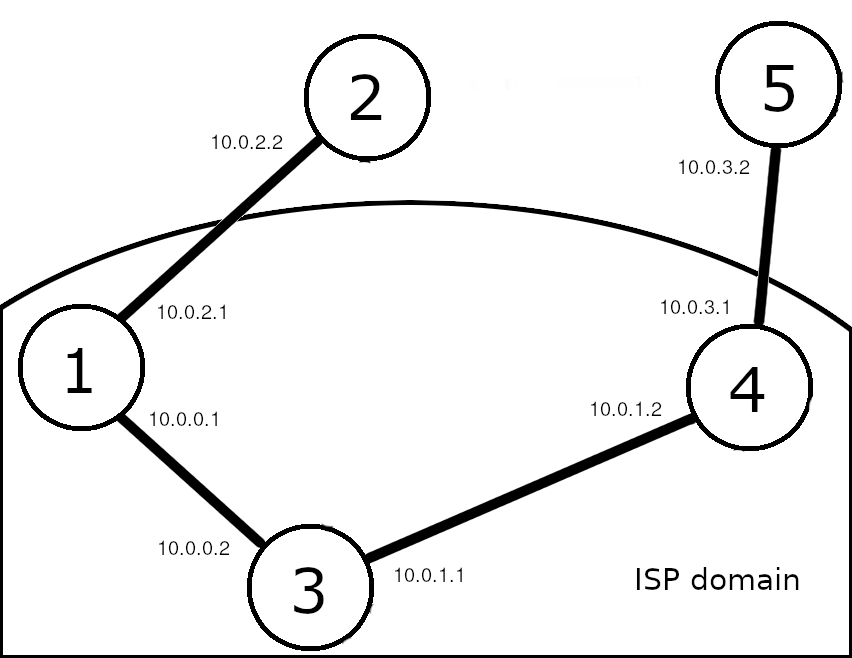
\includegraphics[scale=1.00]{img/topology-boundary.png}
        \caption{Example network topology with ISP boundary}
        \label{fig:example-topology-boundary}
\end{figure}

\begin{table}[H]
\centering
\hspace*{-1.64em}
\begin{tabular}{|l|L|l|l|c|}
    \hline
    \textbf{PID}  & \multicolumn{1}{m{5cm}|}{\textbf{IPv4}}                                                 & \textbf{IPv6}   & \textbf{MAC}      & \textf{priv:my-overlay}  \\ \hline
    1             & \multicolumn{1}{m{5cm}|}{[10.0.0.0/24,10.0.1.0/24, 10.0.2.1/32, 10.0.3.1/32]}           & -                 & D0-9F-BF-2A-00-00/32 & [1, 3, 4]           \\ \hline
    2             & \multicolumn{1}{m{5cm}|}{[10.0.2.2/32]}                                                 & -                 & D0-9F-BF-2A-FE-00/40 & 2                   \\ \hline
    3             & \multicolumn{1}{m{5cm}|}{[10.0.3.2/32]}                                                 & -                 & F8-BB-0B-0A-AA-AA/40 & 5                   \\ \hline
    4             & \multicolumn{1}{m{5cm}|}{0.0.0.0/0}                                                     & ::/0              & 00-00-00-00-00-00/0  & *                   \\ \hline
\end{tabular}
\caption{Example network map referencing Figure \ref{fig:example-topology-boundary}}
\label{table:networkmap-example}
\end{table}

    A cost map contains a list of cost map matrices, with each matrix setting pairwise values between an origin entity and a destination entity.
    If it is a standard cost map, these entities are represented by \glspl{pid} that can be cross-referenced from a network map which this resource depends on, whereas if it is an endpoint cost map, these entities are endpoint addresses which, similar to network maps, include \gls{ipv4}, \gls{ipv6}, \gls{mac} and private endpoint types.
    A matrix must specify the type of cost represented with both their cost type and cost mode, with available options being the ones specified in the ongoing \gls{alto} group's cost metric specification \cite{alto-cost-metrics}.
    Optionally, a cost matrix can specify calendar information about that matrix - similar to the current work in \cite{alto-calendar-cost-map} - which signifies that besides having single-value costs - which are obligatory for any cost matrix - it also contains a time-sensitive list of costs that must be interpreted according to the calendar information provided, and give a chronological overview of what the costs will be in the future.
    If the \gls{isp} contains full topological knowledge of the resource it is sharing, the information that can be provided by the cost maps can be quite detailed.
    Consider the topology in Figure \ref{fig:example-topology} with its five network nodes - from the cost map presented in Figure \ref{table:costmap-example-non-boundary}, one cost matrix depicts a generic "routingcost" cost matrix, depicting routing preference as a shortest path map with a Dijkstra algorithm and hop count as its link cost, and another could provide a "delay-ow" cost matrix, depicting expected one-way delay in milliseconds, as the cumulative calculation of known link delays.

\begin{figure}[H]
        \centering
        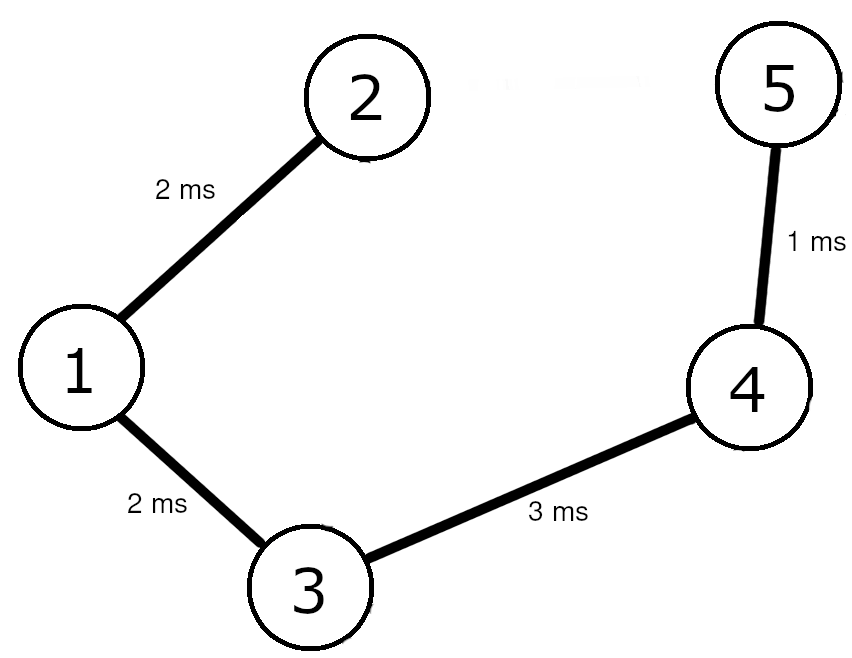
\includegraphics[scale=1.00]{img/topology.png}
        \caption{Example overlay network topology without ISP boundary}
        \label{fig:example-topology}
\end{figure}

\begin{table}[H]
    \centering
    \begin{subtable}{.4\linewidth}
        \centering
        \begin{tabular}{|l|l|l|l|l|l|}
        \hline
        Cost Mode   & \multicolumn{5}{|l|}{routingcost} \\ \hline
        Cost Metric & \multicolumn{5}{|l|}{numerical}   \\ \hline
        From/To     & 1    & 2     & 3   & 4   & 5      \\ \hline
        1           & 0    & 1     & 1   & 2   & 3      \\ \hline
        2           & 1    & 0     & 2   & 3   & 4      \\ \hline
        3           & 1    & 2     & 0   & 1   & 2      \\ \hline
        4           & 2    & 3     & 1   & 0   & 1      \\ \hline
        5           & 3    & 4     & 2   & 1   & 0      \\ \hline
        \end{tabular}
    \caption{Routing cost cost matrix}
    \end{subtable}
    \begin{subtable}{.4\linewidth}
        \centering
        \begin{tabular}{|l|l|l|l|l|l|}
        \hline
        Cost Mode   & \multicolumn{5}{|l|}{delay-ow}    \\ \hline
        Cost Metric & \multicolumn{5}{|l|}{numerical}   \\ \hline
        From/To     & 1    & 2     & 3   & 4   & 5      \\ \hline
        1           & 0    & 2     & 2   & 5   & 6      \\ \hline
        2           & 2    & 0     & 4   & 7   & 8      \\ \hline
        3           & 2    & 4     & 0   & 3   & 4      \\ \hline
        4           & 5    & 7     & 3   & 0   & 1      \\ \hline
        5           & 6    & 8     & 4   & 1   & 0      \\ \hline
        \end{tabular}
    \caption{One way packet delay cost matrix}
    \end{subtable}

    \caption{Example cost map for overlay in Figure \ref{fig:example-topology}}
    \label{table:costmap-example-non-boundary}
\end{table}

    Without either full administrative control or some multi-\gls{alto} domain orchestration mechanism, a single \gls{alto} server instance is restricted to the information it knows.
    Being bound by limited topological knowledge, however, does not necessarily mean that valuable inter-layer cooperation is not possible, and will now be subject of discussion.
    The network map presented previously contains in of itself important information, grouping endpoints into \glspl{pid} that represent network borders - one local to the server, and two representing the peering relationships.
    This is relevant to help clients localize their traffic and would be impossible to derive without \glspl{is} insight.
    Table \ref{table:costmap-example-boundary} provides an example of cost matrices within a single cost map that consider a limited single \gls{alto} server domain topology in Figure \ref{fig:example-topology-boundary}.
    Notice how the \glspl{is} administrative domain is within scope of only three of the five network nodes.
    The \gls{isp} only possesses detailed network status information that regards to nodes "1", "3" and "4", which limits the amount of topological information that can be retrieved and shared to \gls{alto} clients - however, it's still very much possible to dictate routing preferences and gaps in knowledge can be filled with probing measurements to be collected and centralized by the \gls{alto} server to acquire historical performance metrics.
    As can be seen, a generic "routingcost" cost matrix is presented, whose value increases with the associated costs of transferring data through that path, and constructed as the \gls{isp} best sees fit - costs within the \gls{isp} domain are minimal, whereas paths that originate locally and target "PID2" or "PID5" - both requiring the utilization of peering links - are less preferable, with the former being at least twice more preferable than the latter.
    A "delay-ow" cost matrix is also provided, specifying one way packet delay in milliseconds, with the \gls{isp} applying preceding probing measurements between endpoints and averaging the results.
    Finally, a "tput" cost matrix can be seen, specifying expected throughput in bytes per second, with the \gls{isp} applying probing measurements, topological insight, as well as collected feedback of previous application connections that occurred between endpoints to deduce available bandwidth between target points in practice.
    Additionally, the inclusion of cost calendar capabilities to the cost matrix enables users to get a chronological view of bandwidth availability at rush hours, with the single value cost being updated to the present time if a decision needs to be made only considering the current time.
    A similar cost matrix is presented next, that, instead of specifying the throughput costs as dimensional values, does so instead in an ordinal fashion, where the number represents a ranking position in preference, with a lower number representing higher preference.
    This is an alternative that preserves ranking information without requiring from the \gls{isps} the need to concretely specify network status, and instead ordering connections by relative preference, with the option of assigning equal preference to paths that differ in a given order of magnitude that the \gls{isp} sees as negligible.
    In the presented case, locality is correlated with more reliable communications and less operational costs from the \gls{isp}'s point of view, and a concrete better choice exists - regarding routing cost, delay, and throughput - between the two peering connections
    That information can be part of the \gls{alto} system as query-eligible by client applications that can now better optimize their network-related decisions in a mutually beneficial scenario.

\begin{table}
    \centering
    \begin{subtable}{.46\linewidth}
        \centering
        \begin{tabular}{|l|l|l|l|l|l|}
        \hline
        Cost Mode   & \multicolumn{5}{|l|}{routingcost} \\ \hline
        Cost Metric & \multicolumn{5}{|l|}{numerical}   \\ \hline
        From/To     & 1    & 2     & 3   & 4   & 5      \\ \hline
        1           & 0    & 10    & 1   & 2   & 22     \\ \hline
        2           & -    & -     & -   & -   & -      \\ \hline
        3           & 1    & 11    & 0   & 1   & 21     \\ \hline
        4           & 2    & 22    & 1   & 0   & 20     \\ \hline
        5           & -    & -     & -   & -   & -      \\ \hline
        \end{tabular}
    \caption{Routing cost cost matrix}
    \end{subtable}
    \begin{subtable}{.46\linewidth}
        \centering
        \begin{tabular}{|l|l|l|l|l|l|}
        \hline
        Cost Mode   & \multicolumn{5}{|l|}{delay-ow}    \\ \hline
        Cost Metric & \multicolumn{5}{|l|}{numerical}   \\ \hline
        From/To     & 1    & 2     & 3   & 4   & 5      \\ \hline
        1           & 2    & 20    & 1.5 & 3   & 42     \\ \hline
        2           & -    & -     & -   & -   & -      \\ \hline
        3           & 4    & 24    & 2   & 2   & 39     \\ \hline
        4           & 7    & 27    & 2   & 2   & 36     \\ \hline
        5           & -    & -     & -   & -   & -      \\ \hline
        \end{tabular}
    \caption{One way packet delay cost matrix}
    \end{subtable}
    \begin{subtable}{.65\linewidth}
        \centering
        \hspace{-4em}
        \begin{tabular}{|l|l|l|l|l|l|}
        \hline
        Cost Mode   & \multicolumn{5}{|l|}{tput}                       \\ \hline
        Cost Metric & \multicolumn{5}{|l|}{numerical}                  \\ \hline
        From/To     & 1         & 2     & 3        & 4        & 5      \\ \hline
        1           & 256000    & 10000 & 256000   & 256000   & 5000   \\ \hline
        2           & -         & -     & -        & -        & -      \\ \hline
        3           & 256000    & 10000 & 256000   & 256000   & 5000   \\ \hline
        4           & 256000    & 10000 & 256000   & 256000   & 5000   \\ \hline
        5           & -         & -     & -        & -        & -      \\ \hline
        \end{tabular}
    \caption{TCP throughput cost matrix}
    \end{subtable}
    \begin{subtable}{.30\linewidth}
        \centering
        \begin{tabular}{|l|l|l|l|l|l|}
        \hline
        Cost Mode   & \multicolumn{5}{|l|}{tput}                       \\ \hline
        Cost Metric & \multicolumn{5}{|l|}{ordinal}                    \\ \hline
        From/To     & 1         & 2     & 3        & 4        & 5      \\ \hline
        1           & 1         & 2     & 1        & 1        & 3      \\ \hline
        2           & -         & -     & -        & -        & -      \\ \hline
        3           & 1         & 2     & 1        & 1        & 3      \\ \hline
        4           & 1         & 2     & 1        & 1        & 3      \\ \hline
        5           & -         & -     & -        & -        & -      \\ \hline
        \end{tabular}
    \caption{TCP throughput ranking cost matrix}
    \end{subtable}
    \begin{subtable}{1\linewidth}
        \footnotesize
        \centering
        \hspace*{-2em}
        \begin{tabular}{|l|l|l|l|l|l|}
        \hline
        Cost Mode                & \multicolumn{5}{|l|}{tput}                            \\ \hline
        Cost Metric              & \multicolumn{5}{|l|}{numerical}                       \\ \hline
        Calendar Start           & \multicolumn{5}{|l|}{Tue, 20 Sep 2020 17:00:00 GMT}   \\ \hline
        Calendar Interval size   & \multicolumn{5}{|l|}{7200}                            \\ \hline
        Calendar Interval number & \multicolumn{5}{|l|}{6}                               \\ \hline
        From/To                  & 1                    & 2                     & 3                        & 4                   & 5                  \\ \hline
        1                        & (1,[1,1,1,2,2,1])    & (2,[2,2,2,1,1,2])     & (1,[1,1,1,2,2,1])        & (1,[1,1,1,2,2,1])   & (3,[3,3,3,2,2,1])  \\ \hline
        2                        & -                    & -                     & -                        & -                   & -                  \\ \hline
        3                        & (1,[1,1,1,2,2,1])    & (2,[2,2,2,1,2,1])     & (1,[1,1,1,2,1,1])        & (2,[2,2,2,1,1,1])   & (1,[3,1,1,1,1,1])  \\ \hline
        4                        & (1,[1,1,2,2,1,1])    & (1,[2,2,1,1,1,1])     & (1,[1,1,1,1,2,1])        & (2,[1,1,2,2,2,2])   & (3,[3,3,3,3,2,2])  \\ \hline
        5                        & -                    & -                     & -                        & -                   & -                  \\ \hline
        \end{tabular}
    \caption{TCP throughput cost matrix with calendar values}
    \end{subtable}

    \caption{Example cost map for the limited \gls{isp} domain in \ref{fig:example-topology}}
    \label{table:costmap-example-boundary}
\end{table}

    \newpage

    The network status information of an endpoint property map stores the property information of a given endpoint.
    The \gls{alto} working group's protocol specification \cite{alto-protocol} does not directly specify what kind of properties are pondered for this map.
    Following the same design pattern used for the other specified resources, the endpoint property map will have a set of defined properties with associated semantics, and all other properties can be added with the "priv" prefix to designate private properties outside of the considered domain, and thus all semantics and validation rules don't apply.
    Much like the other resources, an endpoint can be identified by an \gls{ipv4}, \gls{ipv6}, \gls{mac} or private overlay address, and the pondered properties are \gls{pid} value, geographical coordinates, connection type (fiber, \gls{adsl}, etc.), server footprint information (total \gls{ram}, \gls{cpu}, and storage), and server status information (what portion of the footprint information is currently available, such as free processing power).
    In practice, a given property could be promoted from a private type to one pondered in the protocol and have a resulting official semantic and validation rules.
    Table \ref{table:example-endpoint-prop} display an example endpoint property map, which is used to store status information relating to servers, identified by their \gls{ipv4} address, that serve the same content.

    \begin{table}[H]
    \centering
    \hspace*{-3.8em}
    \begin{tabular}{|l|l|l|l|l|l|}
    \hline
    Endpoint        & CPU \% & RAM \% & Geographic Coordinates & Connection type & priv:is-mirror \\ \hline
    145.132.164.101 & 22     & 50     & (34.28278,-82.50490)   & Fiber           & False          \\ \hline
    245.217.176.67  & 30     & 45     & (23.24178,-53.51290)   & Fiber           & True           \\ \hline
    48.43.96.168    & 25     & 30     & (55.33218,-12.50490)   & Fiber           & True           \\ \hline
    207.20.148.21   & 10     & 20     & (-23.28121,-22.55530)  & Fiber           & True           \\ \hline
    89.140.253.77   & 5      & 0      & (12.231278,75.70890)   & Fiber           & True           \\ \hline
    \end{tabular}
    \caption{Example endpoint property map for server replicas}
    \label{table:example-endpoint-prop}
    \end{table}

    Finally, as a means to facilitate resource divulgence from servers to clients, there is also included the specification of an \gls{ird}, that is also based from the \gls{alto} working group's protocol specification \cite{alto-protocol}.
    An \gls{ird} can also be thought of as a resource, but instead of sharing network information, it serves as an index of the available resources that a given server provides.
    Each server must have available for query a single \gls{ird}, that lists all the available resources it provides, along with their metadata.
    Each resource attribute must contain the resource's ID, its \gls{http} media type and, if applicable, their capabilities, accepted input media types, and resource dependencies.
    The capabilities identifies, if existing, the cost and property types that are used - being indexed by their unique name, this allows for these to be cross-referenced on further protocol exchanges without need to repeat information.
    Additionally, the resource's capabilities also serve to indicate what resource functionality extensions are enabled - currently applicable for cost maps only, it serves to signal if the cost map has calendared costs - a protocol extension adapted from the work in progress in \cite{alto-calendar-cost-map}, that serves to retrieve calendar cost values, or if the multi-cost extension functionality exists - a protocol extension adapted from \cite{alto-multi-cost}, which lets multiple matrices be requested at once to save on overhead traffic that would otherwise be necessary to request many matrices.
    Two additions are made to the working group's specification - firstly, a description field, which for each resource attribute gives a brief description of what it is about, as it could facilitate resource selection, since such a description could go into detail about appropriate usage guidelines of that resource and suggested use cases; finally, the resource's \gls{acl}, letting a user know beforehand what clearances the given resource has - being a crucial part of the metadata, it seems fitting to go into the \gls{ird}, and has the added benefit of giving the user this piece of information without him having to make resource requests just to, by server reaction, figure out what he can and cannot do.
    A default network map entry must also exist in the \gls{ird}, as per the working group's specification, to serve as a guideline for clients that wish to use the most basic of \gls{isp} endpoint groupings.

    An example \gls{ird} is provided in \ref{table:ird-example}.
    A list of available costs and properties is presented, with their descriptive data discussed above, along with the available resources provided by that server, which contains data useful for their server cluster, as well as a broader-purpose endpoint cost map to query for path connection types and facilitate user selection.
    Finally, a default network map is presented.

\begin{table}[H]
    \centering
        \begin{subtable}{1\linewidth}
        \centering
        \begin{tabular}{|l|l|l|L|}
        \hline
        \bf{Cost ID}     & \bf{Cost Mode}   & \bf{Cost Metric} & \multicolumn{1}{m{5cm}|}{\bf{Description}}                                                                \\ \hline
        routing          & routingcost      & numerical        & \multicolumn{1}{m{5cm}|}{Default routing preference}                                                      \\ \hline
        routing-rank     & routingcost      & ordinal          & \multicolumn{1}{m{5cm}|}{Routing preference by ranking}                                                   \\ \hline
        owd              & delay-ow         & numerical        & \multicolumn{1}{m{5cm}|}{Expected one way delay of a single packet. Based on application statistics}      \\ \hline
        tput-theoretical & tput             & numerical        & \multicolumn{1}{m{5cm}|}{Theoretical maximum available TCP throughput. Based on topological knowledge}    \\ \hline
        tput-practical   & tput             & numerical        & \multicolumn{1}{m{5cm}|}{Practical expected TCP throughput. Based on application statistics}              \\ \hline
        \end{tabular}
        \caption{Available cost types}
        \end{subtable}

        \begin{subtable}{1\linewidth}
        \centering
        \begin{tabular}{|l|l|l|}
        \hline
        \bf{Property ID} & \bf{Property type}         & \bf{Description}                              \\ \hline
        cpu              & CPU                        & Machine's current CPU load                    \\ \hline
        ram              & RAM                        & Machine's currently occupied RAM                \\ \hline
        coord            & geographic-coordinate      & Machine's geographical coordinates            \\ \hline
        connection       & connection-type            & Machine interface's connection type           \\ \hline
        is-mirror        & priv:is-mirror             & Flag stating if machine is a mirror of original server \\ \hline
        \end{tabular}
        \caption{Available property types}
        \end{subtable}

        \begin{subtable}{1\linewidth}
        \centering
        \hspace*{-8em}
        \tiny
        \begin{tabular}{|l|l|l|l|l|l|l|}
        \hline
        Resource ID             & URI                                & Media Type        & Uses           & Accepts                 & Capabilities                                              & Description                                   \\ \hline
        def-nmap          & resources/networkmaps/default      & alto-networkmap   & -              & alto-networkmapfilter   & -                                                         & Default                           \\ \hline
        cluster-costmap         & resources/costmaps/cluster         & alto-costmap      & def-networkmap & alto-costmapfilter      & Costs: {[}routing, routing-rank{]} & For main data center cluster         \\ \hline
        cluster-endprop   & resources/endpointpropmaps/cluster & alto-endpointprop & -              & alto-endpointpropparams & Properties: {[}cpu, ram, coords{]} & For main data center cluster \\ \hline
        client-endcost & resources/endpointcostmaps/        & alto-endpointcost & -              & alto-endpointcostparams & Costs: {[}routing-rank, owd, tput-practical{]}            & For user application guidance       \\ \hline
        \end{tabular}
        \caption{Available resources}
        \end{subtable}
        \begin{subtable}{1\linewidth}
        \centering
        \begin{tabular}{|l|l|l|L|}
        \hline
        \bf{Resource ID} \\ \hline
        def-nmap         \\ \hline
        \end{tabular}
        \caption{Default Network Map}
        \end{subtable}

    \caption{Example of an \gls{alto} server's \gls{ird}}
    \label{table:ird-example}
\end{table}

Further formal specification is not made as it has been extensively done in the \gls{alto} protocol \cite{alto-protocol}, and the proposed system complies to it whilst extending upon the design.

\section{Roles}

\subsection{ALTO Client}

    An \gls{alto} resource consumer is materialized in the architecture in the form of an \gls{alto} client, which can be any entity who is able to interface with an \gls{alto} server to query for \gls{alto} resources.
    Whilst the \gls{alto} working group was initially devised to help increase \gls{p2p}-related traffic localization via the sharing of network information, it now has an increased scope where an ideal client is any application which generates network traffic and would be able to optimize it with aid from an oracle entity with privileged network information.
    Thus, an \gls{alto} client is fit to be implemented in \gls{p2p} applications, and could be embedded in a \gls{p2p} client itself to help with picking neighbouring and content providing nodes, or on a tracker that would accomplish the same goal on behalf of the querying peer.
    Likewise, nodes which are unable to optimally select between other nodes, such as \gls{cdn} edge nodes or content mirrors, could also benefit from oracle guidance, and thus qualify as appropriate \gls{alto} clients.

    Figure \ref{fig:communication-p2p} exemplifies how a cooperative \gls{p2p} application would, acting as an ALTO client, interact with the ALTO server to retrieve relevant network resources to aid their application choice of what candidate peer to consume a service from.
    Firstly, a network map is retrieved to help group endpoints into groupings, and afterwards a cost map is retrieved filtering only the querying peer as source, candidate peers as destinations, and the routing cost and bandwidth cost matrices.
    Acting on this information, the peer chooses the candidate that gives a good balance between \gls{isp} routing cost and path bandwidth, making a decision that should ideally benefit both them and the \gls{isp} that helped provide that information.

\begin{figure}[H]
        \centering
        \hspace*{-0.7em}
        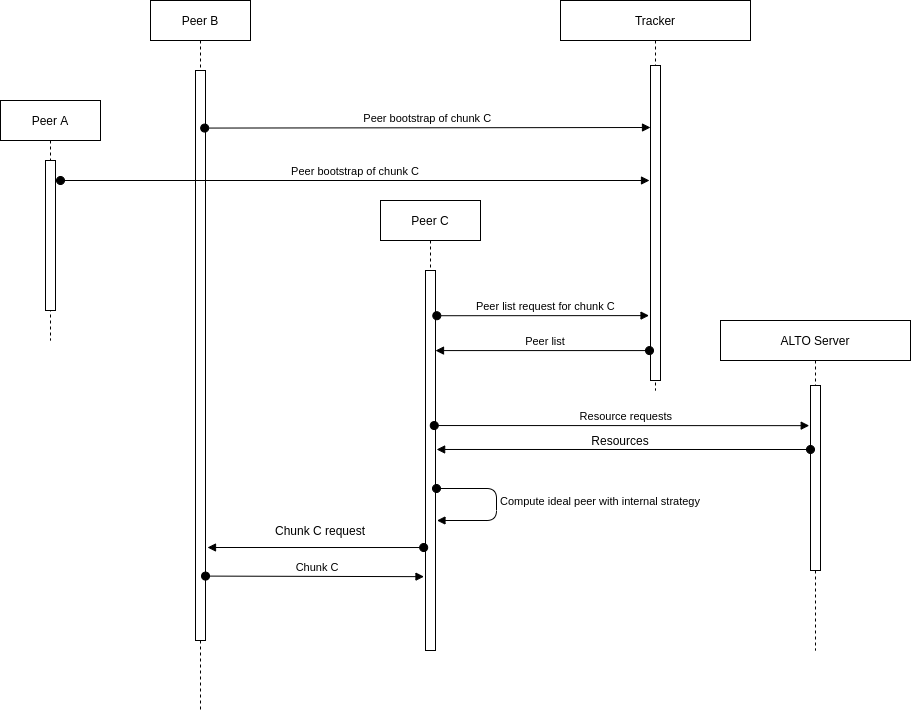
\includegraphics[scale=0.48]{communication-p2p.png}
        \caption{High-level communication diagram of a \gls{p2p} application utilizing \gls{alto}}
        \label{fig:communication-p2p}
\end{figure}

    Figure \ref{fig:communication-tracker} is similar to the previous example, in the sense that it aids a \gls{p2p} application by resorting to \gls{alto}'s guidance, but this time the application-level traffic optimization is made in a way that is transparent to the \gls{p2p} client.
    As a choice to purely localize traffic - as this alone can bring plenty of benefits to both layers - and as a means to minimize protocol modification, it is the tracker that acts as an \gls{alto} client.
    Whenever a request is made by a \gls{p2p} client to retrieve peers serving a given data chunk, the tracker first consults with the \gls{alto} server and retrieves its network map that groups peers within administrative domains - either inside the providing \gls{isp}'s domain, thus the local network, and outside administrative domains, grouped by types of peering connections to different autonomous regions.
    The tracker could use a very simple algorithm to filter out of its candidate pool peers that reside outside of the \gls{isp} region where the requesting \gls{p2p} client resides, if a local alternative exists.
    After packaging a reply to the \gls{p2p} client, the protocol acts normally and traffic could be successfully localized with minimal impact.

\begin{figure}[H]
        \centering
        \hspace*{-1em}
        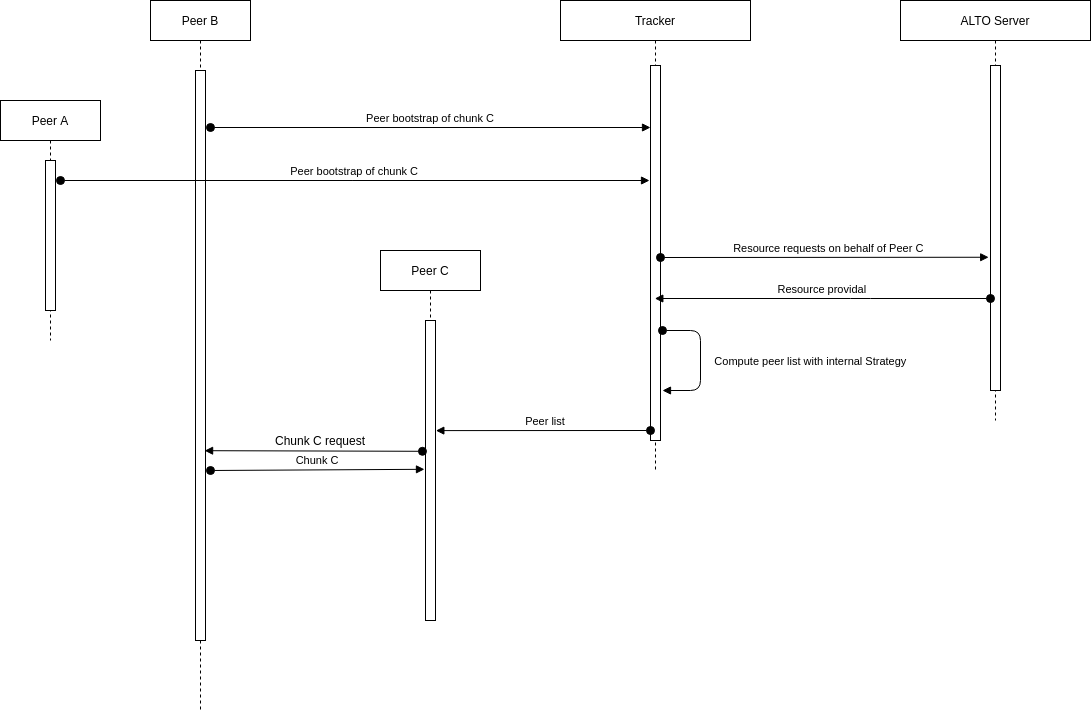
\includegraphics[scale=0.40]{communication-tracker.png}
        \caption{High-level communication diagram of a tracker utilizing \gls{ALTO} by proxy}
        \label{fig:communication-tracker}
\end{figure}

    On the same vein, Figure \ref{fig:cdn-communication} exemplifies how this time a \gls{cdn} controller would use the system to better help its decision in matching \gls{cdn} clients to an edge server on their system.
    To do this, it retrieves a property map to query for server status information, and subsequently retrieves a cost map to query for path information between the \gls{cdn} client and the candidate edge servers.
    Having all the relevant server status information, e.g. available processing and storage resources, as well as connection properties, e.g. max possible bandwidth, latency, and packet loss, the \gls{cdn} controller is in a condition to more optimally redirect his client.

\begin{figure}[H]
        \centering
        \hspace*{-2em}
        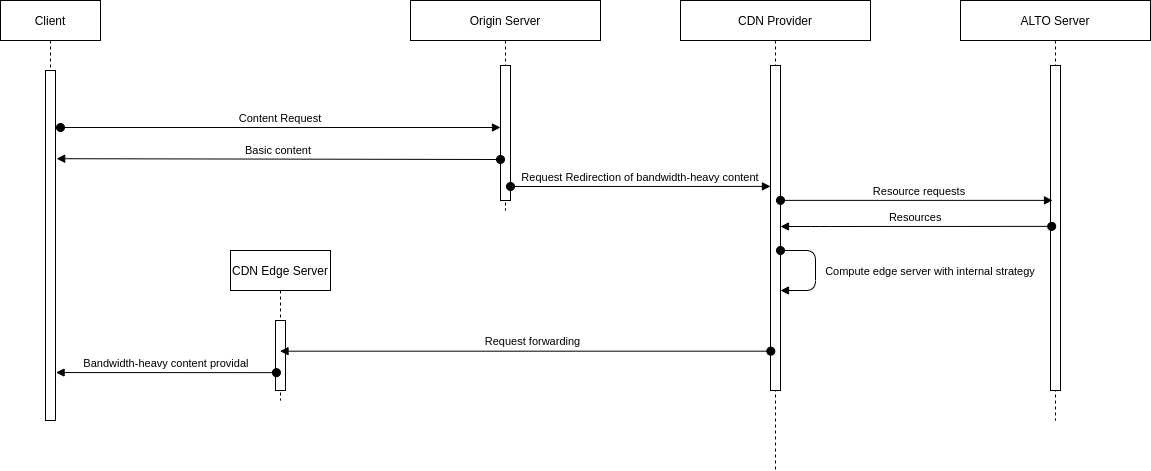
\includegraphics[scale=0.40]{communication-cdn.png}
        \caption{High-level communication diagram of a \gls{cdn} controller utilizing \gls{alto}}
        \label{fig:communication-cdn}
\end{figure}

\subsection{ALTO Server}

    An \gls{alto} resource provider is the \gls{alto} server, an entity that possesses pre-processed and authorized network information in the form of \gls{alto} resources.
    Its job is to store and manage such resources so they can be provided to querying \gls{alto} clients, with the additional responsibilities of data validation and persistence.
    Conceptually, the \gls{alto} server is seen as a single entity, but considering the sensible information that could be stored within it and the influence it has on shaping network traffic, it would not be uncommon for an \gls{alto} server to have a knowledge domain correspondent to the \gls{isp} that owns it.
    Physically, though, the resource provider layer could consist of many interlinked \gls{alto} providers with an increased coverage area of network knowledge.
    Means through which this could occur are further specified in Section \ref{ssec:multi-alto}.

    A listing of available \gls{http} endpoints of the \gls{alto} server interface is available in Table \ref{table:alto-server-api}.
    All resource types hierarchically descend from a "resources" path, and each unique type of resource exposes his own endpoint, with the methods to add, update, remove, and retrieve with and without filter as arguments.
    These methods are subjected to the access control mechanisms discussed in Section \ref{sec:system-roles}, as one should only expect reputable sources to upload and modify data, and only permitted users to query it.

\begin{table}[]
\resizebox{\textwidth}{!}{\begin{tabular}{|l|l|l|}
    \hline
HTTP Verb & Resource                           & Description                                                                                   \\ \hline
GET       & /resources                         & Retrieve the Information Resource Directory for that server                                   \\ \hline
GET       & /resources/networkmaps             & Get summary overview of all available network maps                                            \\ \hline
POST      & /resources/networkmaps/            & Add a new Network Map                                                                         \\ \hline
GET       & /resources/networkmaps/\{id\}      & Get the Network Map with the specified ID                                                     \\ \hline
POST      & /resources/networkmaps/\{id\}      & Get the Network Map with the specified ID, with the applied filter provided in body           \\ \hline
PUT       & /resources/networkmaps/\{id\}      & Modify the contents of a Network Map with the specified ID                                    \\ \hline
DELETE    & /resources/networkmaps/\{id\}      & Remove a Network Map with the specified ID                                                    \\ \hline
GET       & /resources/costmaps                & Get summary overview of all available cost maps                                               \\ \hline
POST      & /resources/costmaps                & Add a new Cost map                                                                            \\ \hline
GET       & /resources/costmaps/\{id\}         & Get the Cost Map with the specified ID                                                        \\ \hline
POST      & /resources/costmaps/\{id\}         & Get the Cost Map with the specified ID, with the applied filter provided in body              \\ \hline
PUT       & /resources/costmaps/\{id\}         & Modify the contents of a Cost Map with the specified ID                                       \\ \hline
DELETE    & /resources/costmaps/\{id\}         & Remove a Cost Map with the specified ID                                                       \\ \hline
GET       & /resources/endpointpropmaps        & Get summary overview of all available Endpoint Property Maps                                  \\ \hline
POST      & /resources/endpointpropmaps        & Add a new Endpoint Property map                                                               \\ \hline
GET       & /resources/endpointpropmaps/\{id\} & Get the Endpoint Property Map with the specified ID                                           \\ \hline
POST      & /resources/endpointpropmaps/\{id\} & Get the Endpoint Property Map with the specified ID, with the applied filter provided in body \\ \hline
PUT       & /resources/endpointpropmaps/\{id\} & Modify the contents of an Endpoint Property Map with the specified ID                         \\ \hline
DELETE    & /resources/endpointpropmaps/\{id\} & Remove an Endpoint Property Map with the specified ID                                         \\ \hline
GET       & /resources/endpointcostmaps        & Get summary overview of all available Endpoint Cost Maps                                      \\ \hline
POST      & /resources/endpointcostmaps        & Add a new Endpoint Cost Map                                                                   \\ \hline
GET       & /resources/endpointcostmaps/\{id\} & Get the Endpoint Cost Map with the specified ID                                               \\ \hline
POST      & /resources/endpointcostmaps/\{id\} & Get the Endpoint Cost Map with the specified ID, with the applied filter provided in body     \\ \hline
PUT       & /resources/endpointcostmaps/\{id\} & Modify the contents of an Endpoint Cost Map with the specified ID                             \\ \hline
DELETE    & /resources/endpointcostmaps/\{id\} & Remove an Endpoint Cost Map with the specified ID                                             \\ \hline
\end{tabular}}
\caption{\gls{alto} server's available endpoints}
\label{table:alto-server-api}
\end{table}


\subsubsection{Resource Filtering}

    Resource filtering is the task through which a resource consumer can pass a filter object to the resource provider that specifies the parameters that the consumer wishes to retrieve specifically.
    With it, there's no need to pass more information to the client than he wishes to get, thus minimizing used network bandwidth and client \gls{cpu} cycles to send and process the resource, respectively.
    The need for filtering becomes greater at a larger system scale - with an increased number of users that query routinely, and resources that can have a massive amount of entries - specifically those that regard to network endpoints - such a mechanism becomes a necessary optimization.
    Keeping with the objective of implementing a fully compatible \gls{alto} protocol as specified by the working group, so will the resource filtering specifications be equal to those already specified in the protocol design \cite{alto-protocol}, thus no further specification will be necessary.

    For clarification, the \gls{alto} server must maintain an endpoint for retrieving all main specified network status resources via filtering, i.e. the server must let the client retrieve \gls{alto} resources with parametrization that dictates what concrete fields must be delivered.
    The types of resource filters considered are the following:

    \begin{itemize}
        \item \textbf{Network Map filter}: List of \gls{pids} of value $PID\_List$, that if empty signifies the entire subset of available \gls{pids}.
            All entries of value:

            \begin{center}
            $(PID, Endpoint\_List)$, $PID \in PID\_List$
            \end{center}

            must be retrieved, and all others must be filtered out.

        \item \textbf{Endpoint Property Map filter}: Pair of list of endpoints and list of properties that must be selected, of value $(Endpoint\_List, Property\_List)$.
            All entries of value

            \begin{center}
            $(Endpoint, Property)$, $Endpoint \in Endpoint\_List \land Property \in Property\_List$
            \end{center}

            must be retrieved, and all others must be filtered out.

        \item \textbf{Cost Map filter}: Tuple of list of source \gls{pids}, list of destination \gls{pids}, list of cost types and list of cost value conditionals of value

            $(SrcPID\_LIST, DstPID\_LIST, CostType\_List, CostValueConditional\_List)$,

            with $CostType\_List > 1$ assuming a multi-cost map extension and the emptiness of any of the lists signifying the entire subset of available values.
            All entries of value

            \begin{center}
            $(Src\_PID, Dst\_PID, Cost\_Type, Cost\_Value)$, $Src\_PID \in SrcPID\_List \land Dst\_PID \in DstPID\_List \land Cost\_Type \in CostType\_List \land satisfies\_atleast\_one(Cost\_Value, CostValueConditional\_List)$
            \end{center}

             must be retrieved, and all other must be filtered out.

         \item \textbf{Endpoint Cost Map filter}: Equal to the cost map filter, but considering a list of source and destination endpoint filters instead of \gls{pids}.
    \end{itemize}

    By analogy, one can consider the \gls{alto} server to act as a remote database with an interface for clients to interact with it, and the filters act as selection statements, such as the "SELECT" method in \gls{sql} databases, to retrieve specific parts of the dataset.
    The filters of cost maps and endpoint cost maps also include a list of premises which themselves are logical operators applied to the candidate cost values.
    Continuing the analogy, these allow the clients to use "WHERE" statements on the numerical cost values that are retrieved.
    In summary, the filter functionality could be explained in the examples shown in Table \ref{table:filter-examples}.

\begin{table}[H]
    \resizebox{\textwidth}{!}{\begin{tabular}{|l|l|l|L|}
    \hline
\bf{HTTP Verb} & \bf{Resource}    & \bf{Body}  & \multicolumn{1}{m{8cm}|}{\bf{Description}} \\ \hline

    POST      & resources/networkmaps/default      & \begin{tabular}[c]{@{}l@{}}\{ \\ "pids": $[$"PID1", "PID2"$]$\\ \} \end{tabular} & \multicolumn{1}{m{8cm}|}{Retrieve an network map with id "default", filtering the entries for \gls{pids} "PID1" and "PID2"} \\ \hline
    POST      & resources/endpointpropmaps/default & \begin{tabular}[c]{@{}l@{}}\{ \\ "endpoints": $[$"ipv4:10.0.0.1", "ipv4:10.0.0.2"$]$,\\  "properties": $[$"CPU", "RAM", "connection-type"$]$ \\ \}\end{tabular}  & \multicolumn{1}{m{8cm}|}{Retrieve an endpoint property map with the id "default", filtering the entries for the properties "CPU", "RAM", and "connection-type" and the \gls{ipv4} endpoints "10.0.0.1" and "10.0.0.2"} \\ \hline
    POST      & resources/costmaps/default         & \begin{tabular}[c]{@{}l@{}}\{ \\ "cost-type": \{ & \quad "cost-mode" : "numerical",\\ \quad "cost-metric": "routingcost" \\ \},\\  "pids": \{ \\ \quad "srcs" : $[$"PID1"$]$,\\ \quad "dsts": $[]$ \\ \quad \} \\ \} \end{tabular} & \multicolumn{1}{m{8cm}|}{Retrieve the cost map with the id "default", filtering the entries for the cost matrix with cost mode "numerical" and cost metric "routingcost", whose entries have source \gls{pid} "PID1" and any destination} \\ \hline
    POST      & resources/costmaps/default         & \begin{tabular}[c]{@{}l@{}}\{ \\ "multi-cost-types": \\ \quad $[$ \\ \quad \{ \\ \quad "cost-mode" : "numerical",\\ \quad "cost-metric": "routingcost" \\ \quad \},\\  \quad \{ \\ \quad "cost-mode": "ordinal",\\ \quad "cost-metric": "routingcost" \\ \quad \} \\ \quad $]$,\\ "pids" : \{ \\ \quad "srcs": $[$"PID1", "PID2"$]$,\\ \quad "dsts" : $[$"PID3"$]$ \\ \quad \} \\ \}\end{tabular} & \multicolumn{1}{m{8cm}|}{Retrieve the cost map with the id "default" and, assuming a multi-cost protocol extension, retrieve both the "numerical" and "ordinal" variations of the "routingcost" metric, whose entries have source \gls{pid} "PID1" or "PID2", and destination "PID3"} \\ \hline
     POST      & resources/costmaps/default         & \begin{tabular}[c]{@{}l@{}}\{ \\ "multi-cost-types": \\ \quad $[$ \\ \quad \{ \\ \quad "cost-mode" : "numerical",\\ \quad "cost-metric": "routingcost" \\ \quad \},\\ \quad \{ \\ \quad "cost-mode": "numerical", \\ \quad "cost-metric": "delay-ow" \\ \quad \} \\ \quad $]$,\\ "calendared": $[$false, true$]$,\\ "pids" : \{ \\ \quad "srcs": $[]$,\\ \quad "dsts" : $[$"PID3"$]$ \\ \quad \}\\ \}\end{tabular}                                                                                           & \multicolumn{1}{m{8cm}|}{Retrieve the cost map with the id "default" and, assuming a multi-cost and cost calendar protocol extensions, retrieve the numerical variants of the "routingcost" and "delay-ow" metrics, requesting a singular value and a calendar value respectively, of all entries whose destination is "PID3"} \\ \hline
     POST      & resources/costmaps/default         & \begin{tabular}[c]{@{}l@{}}\{ \\ "multi-cost-types": \\ \quad $[$ \\ \quad \{ \\ \quad "cost-mode" : "numerical", \\ \quad "cost-metric": "delay-ow" \\ \quad \}, \\ \quad \{ \\ \quad "cost-mode": "ordinal",\\ \quad "cost-metric": "routingcost" \\ \quad \} \\ \quad $]$,\\ "pids" : \{ \\ \quad "srcs" : $[$"PID1"$]$,\\ \quad "dsts" : $[$"PID2"$]$ \\ \quad \},\\ "or-constraints" : \{ \\ \quad $[$ \\ \quad $[$"$[$0$]$ ge 0","$[$0$]$ le 20"$]$,\\ \quad $[$"$[$1$]$ eq 1"$]$ \\ \quad $]$\\ \quad \} \\ \} \end{tabular} & \multicolumn{1}{m{8cm}|}{Retrieve the cost map with the id "default" and, assuming a multi-cost protocol extension, retrieve the "numerical" mode of the "ow-delay" metric and the "ordinal" mode of the "routingcost" metric, whose entires have source "PID1" and destination "PID2", and whose cost values satisfy for a given source and destination pair that either the "ow-delay" is within 0 and 20 ms or it's the number one preferencial "routingcost" value} \\ \hline
\end{tabular}}
\caption{Example \gls{alto} queries with the filtering functionality}
\label{table:filter-examples}
\end{table}


\subsubsection{Server discovery}

    \gls{alto} server discovery, by hand of either network information aggregators or resource consumers, must be done leveraging existing \gls{dns} technologies.
    Each server entity maintains a given domain name, and along it is included the need to also maintain domain records in the chosen \gls{dns} system to map the domain name to the server's \gls{ip} address.
    Much like the choice to utilize \gls{http} as an application protocol, so do the server discovery mechanisms aim to comply with the \gls{alto} working group's philosophy of leveraging existing proven technologies when possible as a means to facilitate development and minimize errors, with the added benefit of extending functionality with the chosen technologies since it is mature and has plenty of options.
    With \gls{dns}, this gives flexibility of either privately configuring domain name to \gls{ip} addresses - much like happens in Linux systems with the "/etc/hosts" file - or its deployment by leveraging existing authoritative \gls{dns} servers.
    Additionally, by working around the existing technology and its specification, one can easily implement load balancing for performance reasons, or, among others, \gls{doh} for preventing eavesdropping, and ensuring both data integrity and host authenticity \cite{dns-https}.
    A similar approach is to be taken for network information aggregator server discovery by part of the network state collectors for the same reasons explained above.

\subsubsection{Inter-server communication}
\label{ssec:multi-alto}

    A glaring gap in the working group's base \gls{alto} protocol is its single administrative applicability domain.
    Meaning, an \gls{alto} server is managed by a single administrative entity - likely an \gls{isp} - and its knowledge domain is limited by the network topology details that the entity knows, which is a subset of the entirety of the Internet's infrastructure.
    In the attempt to fix the server's inability to provide network status information outside its domain, this section overviews mechanisms that enable inter-server communications as a means to expand the capabilities of each domain.

    Firstly, consider how efforts for full resource synchronization could be taken.
    These would be similar to data synchronization mechanisms employed by popular databases to ensure consistency across several server replicas, and could increase availability as well as the serviceability of content nearby clients.
    However, it does not seem to fit this use case - for starters, if all data were to exist redundantly on all servers, that would defeat the purpose of having many administrative domains and thus a single server architecture would suffice; secondly, the architecture is inherently designed to work within a trust domain of selected clients and, because of it, the servers may not even be comfortable with sharing all of its information within other domains to begin with, limiting replication strategies; thirdly, accounting for the amount of users acting on the \gls{alto} system, better scalability could be achieved with a distributed solution that limits information within set boundaries.
    Accounting for these reasons, an inter-server synchronization protocol was designed for servers to negotiate information exchange among themselves, as opposed to one that enabled the synchronization of a single monolithic dataset between servers.

    It is very important that a multi-domain solution assures that each \gls{isp} has full sovereignty over their domain.
    Simply collecting data from each domain and storing it in an third-party entity from which the original source has no control fails to comply to the sovereignty requirement.
    Each \gls{isp} that participates in a multi-domain knowledge system must, at any time, have control over what the information is and who gets access to it, being able to retroactively change its content and the access control policies, respectively.
    This solution will then consider that each \gls{alto} server belonging to the multi-domain orchestration mechanism will compute and store it's data locally,and will have an interface open for data querying from other \gls{alto} servers, being then open to selecting and enforcing their own policies as they see fit, in regards to how and when data is calculated, and who gets access to it.

    To achieve the stated requirements, a "scope" property will be added in the "meta" field of every \gls{alto} resource.
    This property, like the name implies, states the scope of the resource - a "local" resource is no different from those in the base protocol, meaning that it gets calculated and distributed within a single administrative \gls{alto} domain; a "global" resource is essentially virtual, in the sense that it is presented as if it were stored in the server, but instead is dynamically retrieved every time through inter-server communication.
    The decision for this property to be visible in the \gls{ird} was made so it is communicated to the client that a given property can be retrieved as a multi-domain effort - and as such is susceptible to a clash of different \gls{isp} policies and strategies - or as a locally bound resource that will be less prone to inconsistencies, as only a single domain is responsible for managing it.

    To manage the synchronization of globally-scoped \gls{alto} resources, a new entity, the domain synchronizer, was specified.
    This central server will too be an \gls{alto} server, meaning that it will be used to store and manage \gls{alto} resources, although its use is specialized for inter-server synchronization.
    The server maintains property maps, where each of them refers to globally and locally scoped resources, and contains the addresses of the servers that independently store that data and make it available for querying.
    Locally-scoped resource IDs are stored in this server with the addresses of the server's that host it, so that a given \gls{alto} server, whenever asked for a resource which he does not posses, can contact this synchronization database and appropriately redirect a client to a server that contains that information.
    In contrast, globally-scoped resource IDs and their owner's addresses are also stored in this server, so that a given server can know who he must query to retrieve the needed information to locally build the resource to be delivered to the client.

    Listing \ref{lst:example-synchronizer-endpoint-property} shows example data of an endpoint property map for inter-server synchronization.
    Figure \ref{fig:communication-alto-synchronization} shows the required steps taken by a given \gls{alto} server when a client requests for data - in this case an endpoint property map and a cost map - that is globally scoped.

    The required \gls{api} endpoints that an \gls{alto} server must provide for inter-server sharing of resources is no different from the ones they already must provide for clients.
    The only difference is that that these resources contain \glspl{acl} that dictate exclusive action access by authenticated \gls{alto} servers.

\subsection{Network State Provider}

\subsubsection{Network Information Aggregator}

    The network information aggregation layer is the layer that enables the translation of raw topological information - such as the physical attributes of network devices and connections - into processed, query-eligible network knowledge.
    To do so, a very important entity, perhaps the heart of the system as a whole, is the network state collector, which is the supply of network information that is injected, through a network state provisioning protocol, into a network information aggregator.
    This latter entity is then responsible for providing the \gls{alto} resource provider layer with valid information after the raw topological data has been processed - this includes the calculation of optimal paths, the abstraction of network entities, or the injection of static \gls{isp} preferences.
    This pre-processing stage requires input from an \gls{isp} administrator, responsible for acting on the best interest of the \gls{isp} from which the raw topological data originates - by interacting with the network information aggregator, the administrator acts on this network information hub to retrieve from the database a history of retrieved network information, and afterwards manipulate this information to create \gls{alto} resources to its liking - this is where data is transformed utilizing the algorithms the administrator deems fitting, and transforms the raw data to be publishing ready, meaning that it contains an acceptable amount of abstraction not to compromise topological privacy.
    Finally, the administrator defines important meta data that identifies the resource, and defines the access control list to be enforced by the \gls{alto} server.

\subsubsection{Network State Collector}

    Before \gls{alto} resources are provided into the \gls{alto} server by the Network Information Aggregator, the latter needs himself to be provided with raw network status information.
    The \gls{alto} working group has discussed possible sources of raw topological information, including protocols like \gls{igp}, \gls{bgp}, \gls{snmp}, or \gls{netconf}, or databases like the \gls{ted} or \gls{lspd} \cite{alto-deployment-considerations}.
    A protocol needs to exist to interface between the entities that collect and provide the raw topological data, and the Network Information Aggregator that processes it and provides it to the \gls{alto} server.

    The available endpoints supported by the Network Information Aggregator server are presented in Table \ref{table:aggregator-endpoints}.

\begin{table}[H]
\resizebox{\textwidth}{!}{\begin{tabular}{|l|l|l|}
\hline
\bf{HTTP Verb}  & \bf{Resource}                      & \bf{Description}                                               \\ \hline
POST            & /measurements/endpoint             & Add a measured endpoint property value                         \\ \hline
PUT             & /measurements/endpoint/\{id\}      & Modify the contents of a measured endpoint property value      \\ \hline
DELETE          & /measurements/endpoint/\{id\}      & Remove a measured endpoint property value                      \\ \hline
POST            & /measurements/links                & Add a measured link value                                      \\ \hline
PUT             & /measurements/links/\{id\}         & Modify the contents of a measured link value                   \\ \hline
DELETE          & /measurements/links/\{id\}         & Remove a measured link value                                   \\ \hline
POST            & /measurements/group                & Add a measured endpoint grouping                               \\ \hline
PUT             & /measurements/group/\{id\}         & Modify the contents a measured endpoint grouping               \\ \hline
DELETE          & /measurements/group/\{id\}         & Remove a measured endpoint grouping                            \\ \hline
\end{tabular}}
\caption{Network Information Aggregator's available endpoints}
\label{table:aggregator-endpoints}
\end{table}

    An illustrative example on how certain Network State Collectors of given network data could use this endpoint to interface with the Network Information Aggregator is presented on Figure \ref{fig:provisioning-providers}

\begin{figure}[H]
        \centering
        \hspace*{-1em}
        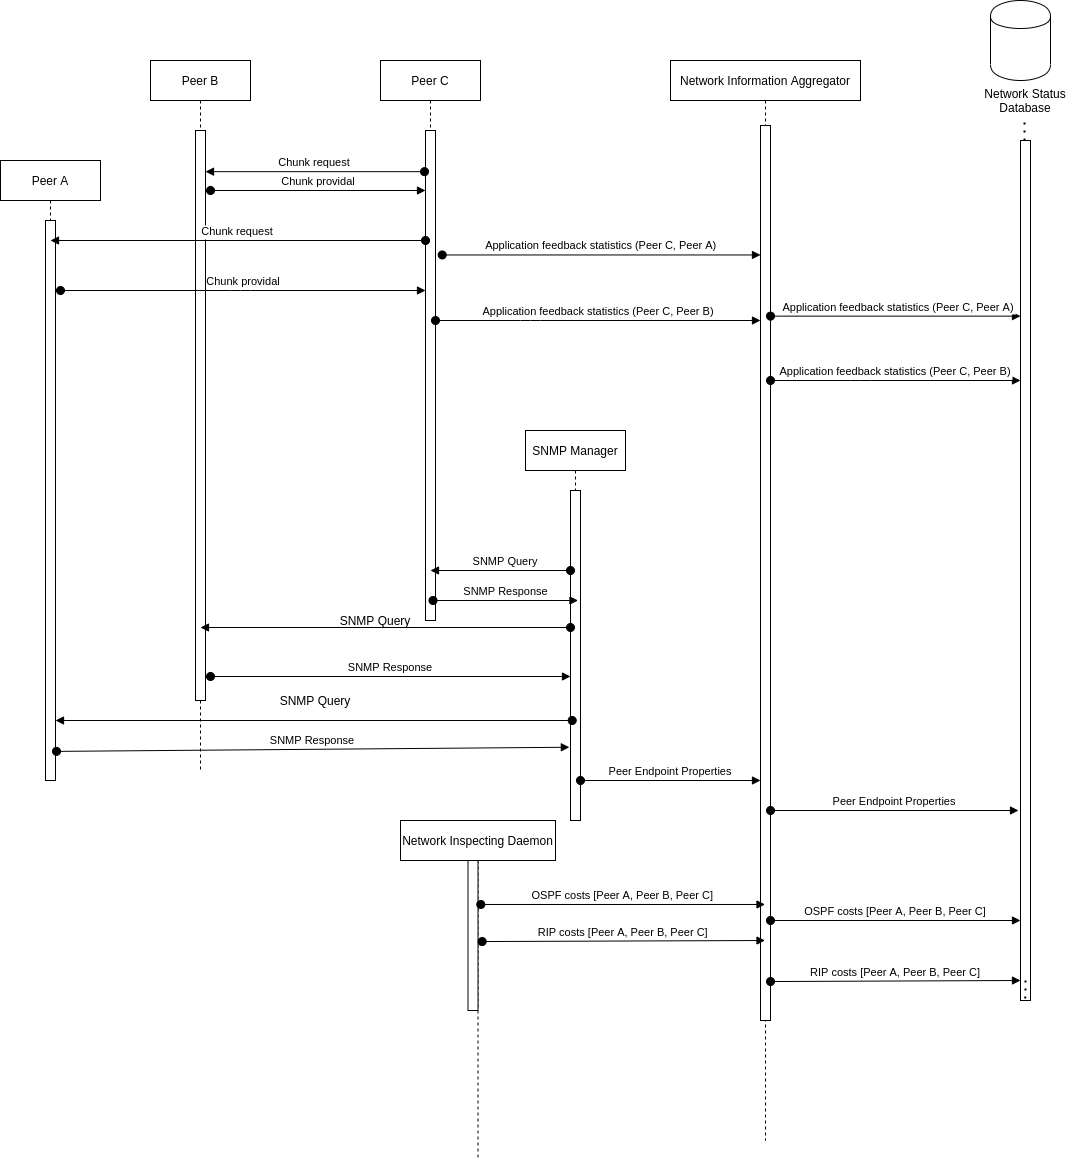
\includegraphics[scale=0.42]{img/communication-info-provisioning-providers.png}
        \caption{Communication diagram of how external network state providers upload information to the network information aggregator}
        \label{fig:provisioning-providers}
\end{figure}


    \textbf{[Network is provided raw, as is, without validation, but validation modules could be provided in the future if a need for it exists. The uploaded information firstly has meta data - which includes the source name (where the data came from, such as an OSPF collector daemon), the time where the measurements were collected, a description, an endpoint or group of endpoints, depending on what the measurement relates to - such as an endpoint property or a cost between two properties or a grouping between N properties, and the measurement itself.]}


\subsubsection{Network Status processing}

    \textbf{[Detail how the ISP uses the information gathered by the network state providers and pre-processes it. This includes, for example, calculating shortest path maps utilizing a Dijkstra algorithm, limiting/changing information to maintain security, adding static ISP policies, and attributing access control policies for that resource]}

    \textbf{Creating a user-friendly network data constructor would be a good future work}

\begin{figure}[H]
        \centering
        \hspace*{-2em}
        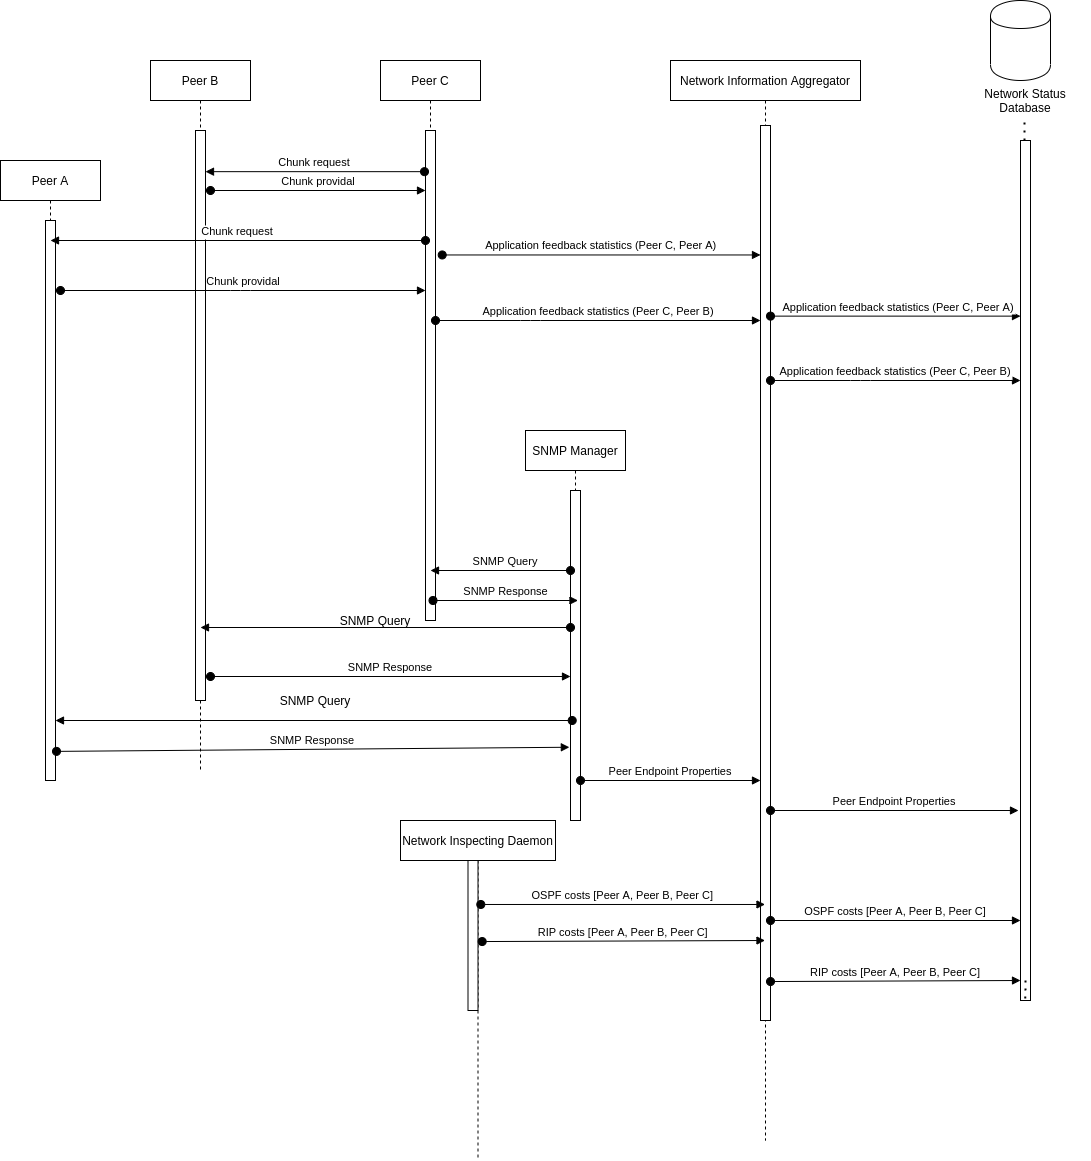
\includegraphics[scale=0.40]{img/communication-info-provisioning-isp.png}
        \caption{Communication diagram of how an ISP administrator pre-processes the gathered network state and uploads it to the ALTO server}
        \label{fig:provisioning-isp}
\end{figure}


%\chapter{Implementation}

    Following the specification, the aim of this chapter is to overview aspects of the implementation stage of the proposed ALTO system.
    Firstly, attention is given to the chosen technologies that were leveraged to get the system from its specification stage into a working product - this includes tools and frameworks in the development and deployment phases, and whose choice greatly delimits the system's properties.
    Secondly, the server is put into spotlight by detailing how it is structured and how it behaves, taking special concern in how object oriented programming was leveraged to maximize modularity and reasoning of the system to facilitate future alterations and extensions.
    Special attention is given to the system's security, where an overview is made what concrete steps were taken to nullify the previously detected potential threats that put into question the viability of the system.

\section{Technologies used}

    Starting the implementation stage of every project, attention must be given into what tools are selected to make it come to fruition.
    These can greatly impact the success of the developed software, and has concrete consequence in its maintenance and future extension.

    The specified system architecture is composed by key entities whose interactions among themselves is clearly defined by interfaces.
    More so, considering the example deployment scenarios, its evident that each entity resides in different topological regions throughout the network, with then the ALTO server, clients, and status providers being scattered through an ISP domain.
    Each entity can then be thought of as a self contained system in of itself who must abide by the proposed interfaces to properly work on the system.
    A logical conclusion to this is that each entity implementation is independent from the next, needing to only assure a common communication channel that all entities within it can properly understand.
    This gives great flexibility in the system implementation as a whole, because different tools can be leveraged to different entities if needed, and such entities that be worked on independently from the rest without impacting the function of the group.

    Regarding the ALTO server, first attention is given to the ALTO resources that must be provided by it.
    They all share some common properties - such as resource id, ACLs, owner, etc. - and functionality - such as the ability to be read and updated, or their permissions modified.
    This similarity is further intensified within groups of resource types, more specifically cost maps - consider how the only concrete difference between and endpoint and a PID cost map is the type of entity the costs refer to, which are endpoint and PID addresses, respectively.
    The sequence of steps that must be taken from the initial point where a client requests a resource up until that resource is provided can be abstracted as the sequential interaction between concrete modules that have a given, self contained, purpose, and communicate with a common interface - an architectural pattern that is a micro version of the one existing in the system, that shares all its properties that were discussed previously.
    Some of these modules would include client request monitoring, its parsing, its validation, database retrieval, database storage, and serialization.
    With all this in mind, an object-oriented programming seems like a proper fit to the complexity pertaining to the ALTO server, especially considering how future extensions would be likely, as very much will be in case of the ALTO working group.
    Working with objects as the base programming entity, many of the highlighted similarities between resources will become easy to be put into evidence, and module encapsulation and interfacing are natural and thus arguably easier to develop and maintain.
    The choice of a language that follows an object-oriented paradigm

    \todo{dynamic vs static}
    \todo{java as a mature programming language that is stable and has many mature libraries}
    \todo{intellij idea}
    \todo{rest api}
    \todo{spring framework as versatile, efficient, http controller support for rest api, security support, dependency injection}
    \todo{unit testing and integration testing}
    \todo{database discussion}
    \todo{mongodb as a scalar choice}
    \todo{database schema}

\section{Server architecture}

    \todo{class diagram}
    \todo{emphasis on single responsibility}
    \todo{discuss packages}
    \todo{code reutilization}
    \todo{interface oriented with code injection}
    \todo{code example}
    \todo{MVC architecture}

\section{Network information aggregator}

\section{Security}
    \todo{concrete protocols used - https, http digest declined over other one}


%\chapter{Experiments}

    The purpose of this chapter is to overview the experiments phase of the project, which consists of the work done to deploy and measure how the system performs in a simulated scenario.
    Whereas the developed unit tests in the implementation stage aim to verify the correct functionality of separate units of code pertaining to the system, the execution of the entire system as a whole to serve a set of hypothetical use cases can help achieve a better grasp on how correct system functionality among all the tested units.
    Adjacent to the goal of testing the system in deployed scenarios, the experiments phase also aims to embed in the simulated environment a list of application scenarios that could leverage the ALTO system to its advantage, and subsequently observe and measure if and how the ALTO server can help the client in the form of provided resources that guide the client in taking application decisions that constitute a win-win scenario between the overlay and underlay.
    As comparison, other known application-network interaction strategies will also be observed and their results measured as a means to compare the impact that these strategies have on both layers.
    Findings on the state of the art of existing interactions and the proposal of the ALTO protocol made on section \ref{sec:state-of-art}, together with the specified system extension on \ref{sec:specification} leads one to believe that a theoretical mutually beneficial scenario exists in an ALTO approach that cannot exist with more asymmetrical means of interaction.
    This chapter, however, puts those theoretical scenarios into a practical environment that could be replicated by those reading this work, and exposing the created scenarios and collected data can corroborate the theoretical conclusions, as well as leaving an opportunity for future discussion on how the system behaved, including its performance, its success in aiding clients, other existing client options that could be a better route, system shortcomings, etc.
    This discussion benefits the ALTO project and can give more maturity to the system as it was put through a simulated deployment against other common strategies.

    The first section displays the chosen technologies for tasks pertaining to the experiments.
    The next section focuses on the required steps taken to setup the testing environment.
    This includes the design and deployment of a network topology in a simulated environment, the creation of mock applications to serve as clients for the system, and the design and deployment of application and network status measurement tools.
    The following section individually overviews the devised scenarios to test in the simulation, and with it experiment specifics such as the initial problem, what strategies will be tested to solve it, how many runs will be made per strategy, and what metrics will be measured.
    Finished the experiments, the following section will display the obtained results that were collected in the simulated environment, and the section after that will discuss these results and how they fare with the theoretical findings.

\section{Technologies Used}

    The Common Open Research Emulator (CORE) \cite{core} was used as a network simulator and represents the backbone of the experiments as a whole, as it represents the network simulator where the experimental environment will be set.
    This tool allows for the creation and emulation of network environments, and with it are included the abilities to construct network topologies and manipulate properties of the member nodes, which can include network routers, switches, and host machines, that will all be used for the designed experiment scenarios.
    Additionally, link connection properties can themselves be customized, as parameters like max bandwidth, packet loss percentage, or packet delay can be meticulously customized, and in fact will be in the upcoming scenarios as a means to simulate a given scenario that may occur in a realistic environment, such as link inefficiency resulting of peak traffic hours.
    Another property that was of great importance for its selection on this work is that, on top of the virtual network environment, arbitrary code can be run on behalf of a given entity and can be addressed to another, acting as if it were an actual network.
    This will be leveraged to run software pre-packaged in the emulator, such as routing protocols that are essential for the correct expected behavior of a simulator network, but also to schedule software execution that was developed for this work, which includes the ALTO server, network state providers - e.g., probing daemons and application feedback collectors - and system clients for the P2P and HTTP mock applications that will be devised to play out a particular experiment scenario, and which will have embedded into it an ALTO client to interface with the server for council.
    As the simulation tool runs on Linux and builds a simulated network that behaves very much like a real one, well known real-application tools can be used on top of it in other needed areas, including the deployment and measuring phases, which gives plenty of flexibility on tool selection.

    Python \cite{python} will be utilized to implement all simple software prototypes whose purpose is uniquely to test the application in a real scenario.
    This includes the P2P file-transfering applications, the HTTP servers and clients, and the throughput-intensive activities done by the data servers.
    Appended to this will also be the task of application monitoring, which includes the retrieval of performance statistics - doing so in the application's code itself, instead of using external tools, because more fine grained access exists and individual tasks can be monitored for how long and how well they perform.
    The choice of this programming language over others is simply that these software prototypes are not intended to be highly optimized, nor are they to be complex.
    Instead, their mode of operation is supposed to be simple in nature, to remove complex variables that might make the experiment results harder to interpret, and to make reasoning and replication of experiment results easier.
    Python seems then like a good fit due to its easy syntax, its interpreted nature that skips work that would otherwise be needed for compilation that might increase peformance - but is not needed - and, finally, its massive collection of helpful libraries.
    For these reasons will too Python be chosen to generate visual graphics reflective of the raw network and application statistics to be collected by other tools.

    Finally, a tool was selected for the task of network monitoring, to collect network data representative of the impact that a given application strategy had towards the infrastructure.
    To this goal, vnStat \cite{vnstat} was chosen, a command line utility to measure network traffic on an interface basis, over given periods of time.
    This application retrieves network interface statistics provided directly by the kernel, and thus performs no traffic sniffing.
    This is not problematic as this level of detail is not needed for the designed experiments, and instead interface statistics that inform on data flow influx and outflux are sufficient.
    Finally, with vnStat being a command line utility, there is the additional bonus that deployment and orchestration are facilitated with scripting.

    \textbf{[python's SimpleHTTPServer module will be leveraged as an HTTP server, and a similar module will be used for FTP file transfers.]}

\section{Setup}

    Figure \ref{fig:test-topology} displays the topology that will act as the main environment for all the devised experiments.
    It was designed with the intent of reflecting the nature of the Internet, in particular with it being an aggregation of multiple, heterogenous, domains, each with their own topological properties and internal policies, with them being administrated by different organizations.
    As can there be seen, a single backbone network - AS 0 - provides connectivity between many ASs and, to do its job correctly, a high degree of path redundancy exists between its edge routers, and the links have better capabilities that those associated with stub networks.
    AS 1 is a simple topological structure consisting of five PCs and and three dedicated servers, connected with the help of switches and routers, that eventually connect to a single edge router that connects to the backbone.
    AS 2 is representative of a data center with two OSPF areas, both constructed with a hierarchical organization common for data center networks.
    Links in these regions are also highly capable and high traffic peak times are expected to occur.
    AS 3 is a slightly more complex stub network compared to AS 1, but has the same structure, with the adition of having three OSPF areas instead of one, and a variety of nodes and links with different properties - for example, the links in area A are generally better, whilst area C has wireless connections in it that are expected to have worse performance and be less reliable.
    Finally, AS 4 connects directly with AS 3, meaning that the latter acts also as a transit AS, being the only access point towards the rest of the network.
    Similarly to AS 3, it consists of a stub network accessed by many end users and some servers, and both node and link properties vary accordingly.

    \todo{Add labels to autonomous systems and link and node properties}

    \begin{figure}[ht]
    \centering
    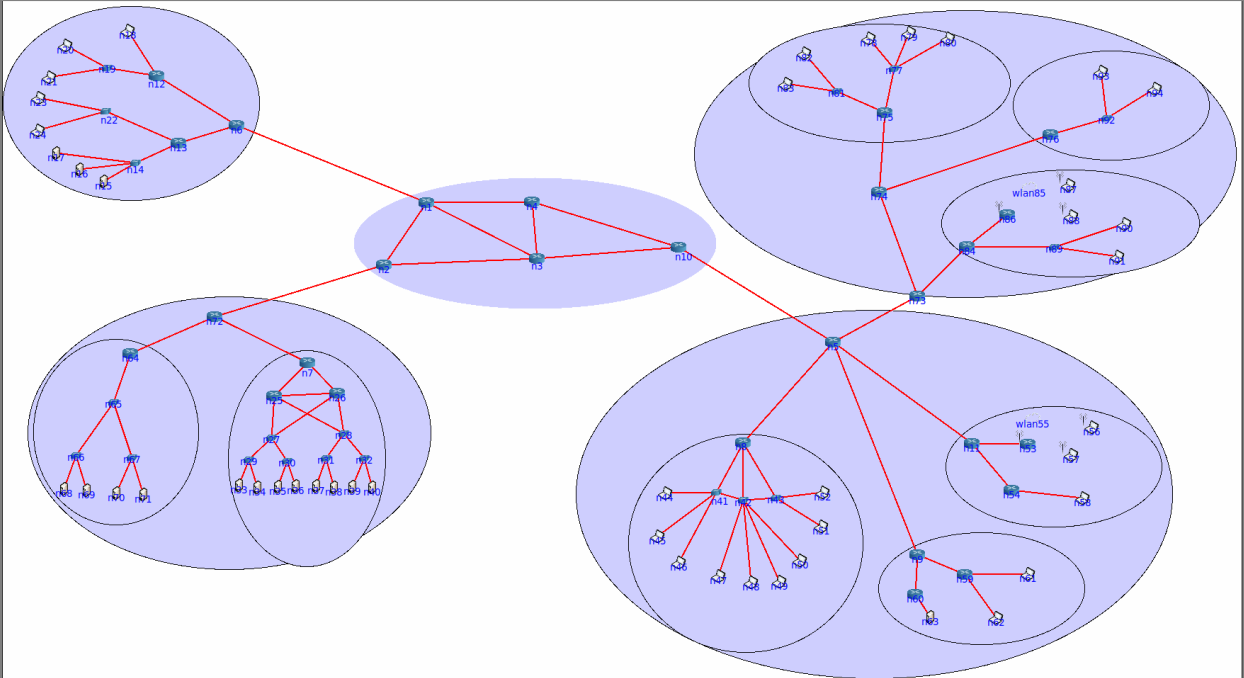
\includegraphics[scale=0.5]{img/test-topology.png}
    \label{fig:test-topology}
    \caption{Simulated topology environment}
    \end{figure}



    Each node on the network has a given purpose that is represented as a node label, and likewise are link labels used to specificy connection properties.
    Unless stated otherwise with these labels, all other properties are equal throughout the network.
    Some pre-packaged CORE services need to be enabled to assure network connectivity - mainly OSPFv3 and BGP - and scripting is used to, at the beginning of the simulation, bootstrap programs in specific nodes.
    This is done by leveraging the command line utility vcmd that runs specificed commands in control channels that are created at runtime by CORE - for example, the following command executes a ping command to address 10.0.0.1 with origins on node P2P-Cli-1 and on simulation session 12345:

    \begin{center}
    \begin{tabular}{c}
    \begin{lstlisting}[caption=Execution of an example command through the control channel of a given node, language=bash]
        $ vcmd -c /tmp/pycore.12345/P2P-Client-1 -- ping 10.0.0.1
    \end{lstlisting}
    \end{tabular}
    \end{center}

\section{Scenarios}

\subsection{Single ALTO administrative domain}

    The following experiments will consider a single ALTO server that only has administrative control of the AS it resides.
    It thus possesses no network topological details outside of his domain, working only with what it knows and what it can derive from the outside.

\subsubsection{Scenario 1 - P2P file sharing}
\textbf{Description:} All "Cli-N" nodes in the network, with N from 1 to N, actively serve all 10 equally sized fragments of a 1GB file to other peers, and the bootstrapping method includes informing the tracker about what file fragments they serve.
    "CliN-1" wishes to retrieve that file, and to do so he firstly contacts "Tracker" for tracking information about that file, that contains a mapping between a fragment ID and suggested peer, alongside with the file's checksum.
    After retreving this mapping, the client will sequencially request each fragment from the appointed peer, and afterwards merge all the fragments into a single file and validates that the calculated checksum matches the tracker's.
    An ALTO server is in the same AS and maintains a network map resource that groups endpoint addresses within locality - per OSPF area in the most specific pids, inside that AS in another, and anything else in another.


\textbf{Variables:} The variable actions to be tested are how the tracker selects a candidate peer to serve a fragment to the requesting peer.
Table \ref{table:s1-tracker-methods} displays the different tracker algorithms that will be tested for the task of peer matching.

\begin{table}[]
\begin{tabular}{ll}
Tracker Algorithm & Description                                                                                                                                                                                                \\
Random            & Randomly select among all available peers                                                                                                                                                                  \\
ALTO              & Retrieve a network map from its ALTO server and discover the attributed PID to both request and candidate clients, choosing randomly between the candidate peers that share the same PID as the candidate.
\end{tabular}
\label{table:s1-tracker-methods}
\end{table}

\textbf{Measurements:} Table \ref{table:s1-measurements} presents the measurements that will be collected during the experiment runs.

\begin{table}[]
\begin{tabular}{lll}
Measurement     & Units     & Description                                                  \\
Transfer Time   & Seconds   & Total amount of time required to transfer all file fragments \\
Network Traffic & Megabytes & Total amount of traffic that passed through the network
\end{tabular}
\label{table:s1-measurements}
\end{table}

\textbf{[Notes: The P2P client has no reasonable way to, without ISP cooperation, know that peers reside within network locality. A cited study used RTT heuristics that assumed that high RTT values exist in inter-ISP links, which may not always be the case. Randomly selecting is poor at optimal choice, but at the very least has potential for load balancing, something that the tracker itself can attempt to do on a per-locality basis, joining a best of both worlds. Leveraing only a network map to communicate peer locality is quick and takes little memory, and further experiments will add cost maps on top of it to mix both locality standards and QoS needs.]}


\subsubsection{HTTP file sharing}

\textbf{Description: } All "HTTP-N" nodes, with N from 1 to N, are HTTP servers and serve a 1GB file to querying clients.
Cli-N has a file that contains the address of all of these mirror servers on the network that can provide that given file to him.
The HTTP servers reside in the same AS, and that ALTO server maintains a network map that groups server regions of similar properties, an endpoint property map that provides real-time status information that includes current cpu and memory load, as well as a cost map providing throughput and delay costs that are compiled from voluntarily provided application performance statistics, as well as a routing cost specifying ISP preference.

\textbf{Variables: } The variable action to be tested is how the HTTP client selects between all known server mirrors that serve the desired file.
Table \ref{table:s2-clients-methods} displays the different client algorithms that will be tested for the task of server selection.

\begin{table}[]
\begin{tabular}{ll}
Client Algorithm & Description                                                                                                                                                                                                \\
Random            & Randomly select among all available servers                                                                                                                                                                  \\
Probe             & Probe for available TCP throughput and existing delay between all available servers, and select the one with most throughput with delay below 20 ms
                                                             \\
ALTO              & Retrieve a network map, endpoint property map, and cost map from the ALTO server in the HTTP servers AS, and choose, if possible, a server that is not overloaded - i.e., whose memory and cpu loads are not past 90\% - whose delay is below 20ms, and which has an historical throughtput of 30 Mbps or more.
If multiple servers match these requirements, choose the one that has the least routing cost among them.
\end{tabular}
\label{table:s1-tracker-methods}
\end{table}

\textbf{Measurements:} Table \ref{table:s2-measurements} presents the measurements that will be collected during the experiment runs.

\begin{table}[]
\begin{tabular}{lll}
Measurement         & Units      & Description                                                  \\
Transfer Time       & Seconds    & Total amount of time required to transfer the requested file \\
CPU Server Load     & Percentage & Average CPU load of all mirror servers \\
Memory Server Load  & Percentage & Average Memory load of all mirror servers \\
Network Traffic     & Megabytes  & Total amount of traffic that passed through the network
\end{tabular}
\label{table:s2-measurements}
\end{table}

\textbf{[Notes: The ALTO method has better data on three fronts: it has a historical and statistical record of connection quality between clients and servers, which will probably be more mature than a ad-hoc probing of the network at that given time; it has server property information regarding status (cpu and memory load, for example) that the client can't retrieve otherwise; it has ISP routing costs that give ISP insight on what choice would be more economically sound for them. The assumption is that the ALTO approach will have better application performance and better network resource utilization because the information retrieved tells a bigger picture than a simple probing for tcp througput and delay. Additionally, if every client were to perform adhoc measurements to pick a client, considerable network traffic overhead will exist, specially with a bigger scale of clients. By centralizing this information as historical and statistical data, and adding into it routing costs that only the ISP could derive, a more mature choice can exist that favors both parties. The old way of manually choosing server mirrors, for example for linux distributions, that end up just being 'let me choose the first one i see that is on my country', can be argued to be objectively worse than adding a ISP cooperative module.]}


\subsubsection{Bulk FTP transfers}

\textbf{Description:} Servers in the Data server AS want to schedule big data transfers between themselves as a form of backup.
These happen routinely, and take a predictable amount of time.
Performing these backups heavily impacts the ability of all servers in that data center to serve clients, because that subnetwork will be utilizing a lot of its resources to achieve that goal.
"Cli-N" wishes to retrieve a single 1GB file, and contains a file that lists all available mirrors and their address.
The data center administrator maintains a cost map calendar where he registers all scheduled backup transfers with two purposes: to keep track of all scheduled transfers so further ones cna be schedules as to not clash with pre-reserved ones, and to signal to ALTO clients when QoS levels to those servers are expected to degrade.

\textbf{Variables: } The variable action to be tested is how the HTTP client selects between all known server mirrors that serve the desired file.
Table \ref{table:s4-clients-methods} displays the different client algorithms that will be tested for the task of server selection.

\begin{table}[]
\begin{tabular}{ll}
Client Algorithm & Description                                                                                                                                                                                                \\
Random            & Randomly select among all available servers                                                                                                                                                                  \\
Probe             & Probe for available TCP throughput and existing delay between all available servers, and select the one with most throughput with delay below 20 ms
                                                             \\
ALTO              & Retrieve a network map and cost map from the ALTO server in the HTTP servers AS, and choose the one that maximizes throughput in the calendar entry where the transfer will occur.
\end{tabular}
\label{table:s5-tracker-methods}
\end{table}

\textbf{Measurements:} Table \ref{table:s1-measurements} presents the measurements that will be collected during the experiment runs.

\begin{table}[]
\begin{tabular}{lll}
Measurement     & Units     & Description                                                  \\
Transfer Time   & Seconds   & Total amount of time required to transfer all file fragments \\
Network Traffic & Megabytes & Total amount of traffic that passed through the network
\end{tabular}
\label{table:s1-measurements}
\end{table}

\subsection{Multi ALTO administrative domains}

    The following experiments assume that the ALTO synchronization protocol is in place and allows multiple servers to maintain globally scoped resources that can be shared to clients.

\subsubsection{P2P file transfer}

\textbf{Description:} Similar to the single domain counterpart, all "Cli-n" nodes in the network, with N from 1 to N, actively serve all 10 equally sized fragments of a 1GB file to other peers, informing the tracker of their availability to do so.
"CliN-1" wishes to retrieve that file, and to do so firstly contacts "Tracker" for tracking information about that file, that contains a mapping between fragment ID and suggested peer, alongside with the file's checksum.
    After retreving this mapping, the client will sequencially request each fragment from the appointed peer, and afterwards merge all the fragments into a single file and validates that the calculated checksum matches the tracker's.
    Each AS has an ALTO server operating with administrative control and topological insight of their own domain, and they together maintain a single cost map with global scope.

\textbf{Variables: } The variable actions to be tested are how the tracker selects a candidate peer to serve a fragment to the requesting peer.
Table \ref{table:s-tracker-methods} displays the different tracker algorithms that will be tested for the task of peer matching.

\begin{table}[]
\begin{tabular}{ll}
Tracker Algorithm & Description                                                                                                                                                                                                \\
Random            & Randomly select among all available peers                                                                                                                                                                  \\
ALTO              & Retrieve an endpoint cost map from its ALTO server that displays cumulative delay, available throughput, and routing cost between peers as a combined synchronization effort between ALTO domains.
Choose the candidate peer whose delay does is, if possible, below 20ms, with a throughput of 30 Mbps or more.
If multiple candidate peers fulfill these requirements, choose the one with the least amount of routing cost.
\end{tabular}
\label{table:s1-tracker-methods}
\end{table}

\textbf{Measurements:} Table \ref{table:s1-measurements} presents the measurements that will be collected during the experiment runs.

\begin{table}[]
\begin{tabular}{lll}
Measurement     & Units     & Description                                                  \\
Transfer Time   & Seconds   & Total amount of time required to transfer all file fragments \\
Network Traffic & Megabytes & Total amount of traffic that passed through the network
\end{tabular}
\label{table:s1-measurements}
\end{table}

\subsubsection{P2P media streaming}

\texbtf{Description: } All "Cli-N" nodes, with N from 1 to N, allow for real-time streaming of a given piece of media.
"Cli-N" has a file containing a list of all available peer addresses that he can request a feed to.

\textbf{Variables: } The variable actions to be tested are how the client selects a candidate peer to request a stream from.

\textbf{[Methods: a) ALTO server maintains a multi-domain throughput, delay and packet loss calendared cost maps that were result of historical and statistical measurements from previous users of that media streaming application that volunteered performance statistics. Routingcost calendared cost map is also added by the ISPs to reflect preference in routing. b) Randomly select peer. c) Choose peer with least RTT, with the heuristic that smallest probe delay allows for better real-time streaming experience d) Randomly select peer and, whenever QoS measurements are degraded for too long, choose another ano - and continuously apply this adaptive peer selective mechanism that essentially "brute forces" the best peer]}
\textbf{[Notes: Again, the ALTO approach is the only one that allows clients to make choices that are inline with ISP's economical and administrative needs. Moreso, the ALTO server has a centralized repository for historical and statistical performance results that occured in that media application, that show a trend in what subnetworks become more loaded over time. ISP probing by the network can also more quickly detect link bottlenecks and quickly upload that data as cost maps, whilst deducing that information without ISP aid would require more probing traffic, and would take considerably longer. Both probing attempts and "brute force" attempts are more harduous and considering the real-time QoS levels of the media streaming application, will considerably degrade application performance. A network-aware and statistical repository solution like ALTO allows one to make the better decision, more quickly, with a mutually beneficial outcome.]}

\section{Results}
\section{Discussion}


%\input{chapters/conclusion

\bookmarksetup{startatroot} % Ends last part.
\addtocontents{toc}{\bigskip} % Making the table of contents look good.

\bibliographystyle{plain}
\bibliography{dissertation}

\printindex

\umappendix{Appendix}

\chapter{Support material}

%\chapter{Details of results}

%\chapter{Listings}

%\chapter{Tooling}

%Anyone using \Latex\ should consider having a look at \TUG,
	%the \tug{\TeX\ Users Group}


% Back Cover -------------------------------------------
\umbackcover{
	NB: place here information about funding, FCT project, etc in which the work is framed. Leave empty otherwise.
	}

\end{document}
